\documentclass[
documentsize = a4, % a4 | octavo
font = cmr, % cmr | utopia | times
typesize = 11, % 9 | 10 | 11 | 12 | 14
printmode = true,
onehalfspacing = true,
language = en, % en | es
titlepage = udciccp, % none | udc | udciccp
degree = pt, % phd | msc | pt
dedication = true,
acknowledgements = true,
abstract-en = true,
abstract-es = false,
abstract-ga = false,
epigraphs = true,
toc = true,
lof = true,
lot = true,
frontmatterintoc = false,
notation = false,
minimal = false,
]{UDCthesis}

\title{An study about the collapse of adhesively bonded crash boxes}
\author{Luis Pire Pardo}
\supervisor{Jacobo Díaz García}
\cosupervisor{Luis Esteban Romera Rodríguez}
\date{2016}

\usepackage{enumitem}
\usepackage{pdfpages}
\usepackage{minted}

\addbibresource{./bib.bib}

\begin{document}

\newacronym{SEA}{SEA}{specific energy absorption}
\newacronym{Ea}{$E_{a}$}{energy absorption}
\newacronym{Pk}{$P_{k}$}{peak force}
\newacronym[longplural={quadratic nominal stress criteria}]{quads}{Quads}{quadratic nominal stress criterion}
\newacronym{COH3D}{COH3D}{3D cohesive element}
\newacronym{SLJ}{SLJ}{single-lap joint}
\newacronym{VCCT}{VCCT}{virtual crack closure technique}
\newacronym{FEM}{FEM}{finite element method}
\newacronym{XFEM}{XFEM}{extended finite element method}
\newacronym{LEFM}{LEFM}{linear elastic fracture mechanics}
\newacronym[longplural={degrees of freedom}]{DOF}{DOF}{degree of freedom}
\newacronym{F-D}{F-D}{force-displacement curve}
\newacronym{HPC}{HPC}{high-performance computer}
\newacronym{TcT}{$Tc_{Total}$}{total computational time}
\newacronym{SDT}{${\Delta}t_{stable}$}{stable time increment}
\newacronym{SD}{SD}{standard deviation}

\begin{abstracten}
Crashworthy elements are essential devices for passenger safety in case of vehicle impact. Their objective is to absorb the greatest amount of energy during the crash with the lowest transmitted force possible to the occupants and surrounding structures, specially the maximum peak force.

These devices are usually made of several pieces, requiring a union between them. In this work, adhesive joints have been studied as an alternative to conventional mechanical joints. In the modelled crash boxes, two steel adherends are bonded together generating a square section tube with flanges and different layouts in which the union is performed with adhesive. Then, the tube is crushed on impact conditions. The numerical model has been parametrized in order to allow future optimization.

Adhesive properties have been taken from literature, including a precise damage model for it, which is also a energy dissipation mechanism. The crash tube required of certain stabilization mechanisms in order to achieve a desired collapse mechanism. A focus was set in the stability of the collapse, as it has influence on several parameters of interest of the resulting crush process.

The crash boxes performance is measured and interpreted through the absorbed energy, $E_{a}$, and the force-displacement curve. The deformation pattern is also studied, being the bending wave formation the main energy dissipation mechanism, although unexpected collapses are found, resulting in undesired output parameters. The energy absorption share of each part is also studied.
\end{abstracten}

%\begin{abstractes}
%El abstracto
%\end{abstractes}

%\begin{abstractga}
%O abstrato
%\end{abstractga}

\begin{acknowledgements}
The author would like to mention some people and institutions to whom holds a very grateful feeling for having been key for the development of this work.

In the very first place Dr. Jacobo Díaz García and Dr. Luis Romera Rodríguez, for the work, help and patience dedicated to me. I will always remember this introduction to the research labour lead by them, and the constant support provided.

It must be mentioned that part of this work is based on developments previously carried out by Dr. Miguel Costas Piñó, who also helped and gave me his time for this study.

In the same vein, the rest of professors and interns of the Grupo de Mecánica de Estructuras (GME), but specially PhD candidate Javier Paz Méndez for his support and helping hands.

In other line, I would also like to mention Dr. María del Carmen Serna Moreno, from Universidad de Castilla-La Mancha, and Dr. Alessandro Scattina, from Politecnico di Torino, for answering my mails giving a helping hand.

Although it may seem eccentric, I would like to mention the Stack Overflow, Python developers and Wikipedia communities for my constant consultations made on typing Python and \LaTeX{} code. The owner of the IP 129.97.46.200 should be mentioned as I have accessed through it to the Abaqus Manual a thousand times.

Finally, I would like to mention my closest family and friends, for supporting me every time they had seen me working on this project.
\end{acknowledgements}

\begin{dedication}
To my mother and father
\end{dedication}

\chapter{Introduction}
\label{0}

Security is a key issue on vehicle design nowadays, and crashworthy elements are required to absorb the energy during a crash and minimize the effects on the occupants. Crash boxes are devices equipped by vehicles that are designed to absorb the impact through deformation in order to protect the vehicle passengers. They are usually tube shaped and made of several pieces that require bonding. This bonding can be also a valid dissipation mechanism, apart from being a way of obtaining low-weight unions.

On the other hand, structural adhesives have improved their mechanical properties in recent years and now can be used with confidence in heavy duty applications. Adhesive unions present themselves as a promising solution for bonding manufacture, thanks to their properties and last years improvements on these. Interest on them is also raising up in scientific fields thanks to these enhancements and to the recent development of validated numerical models.
\begin{figure}
	\centering
	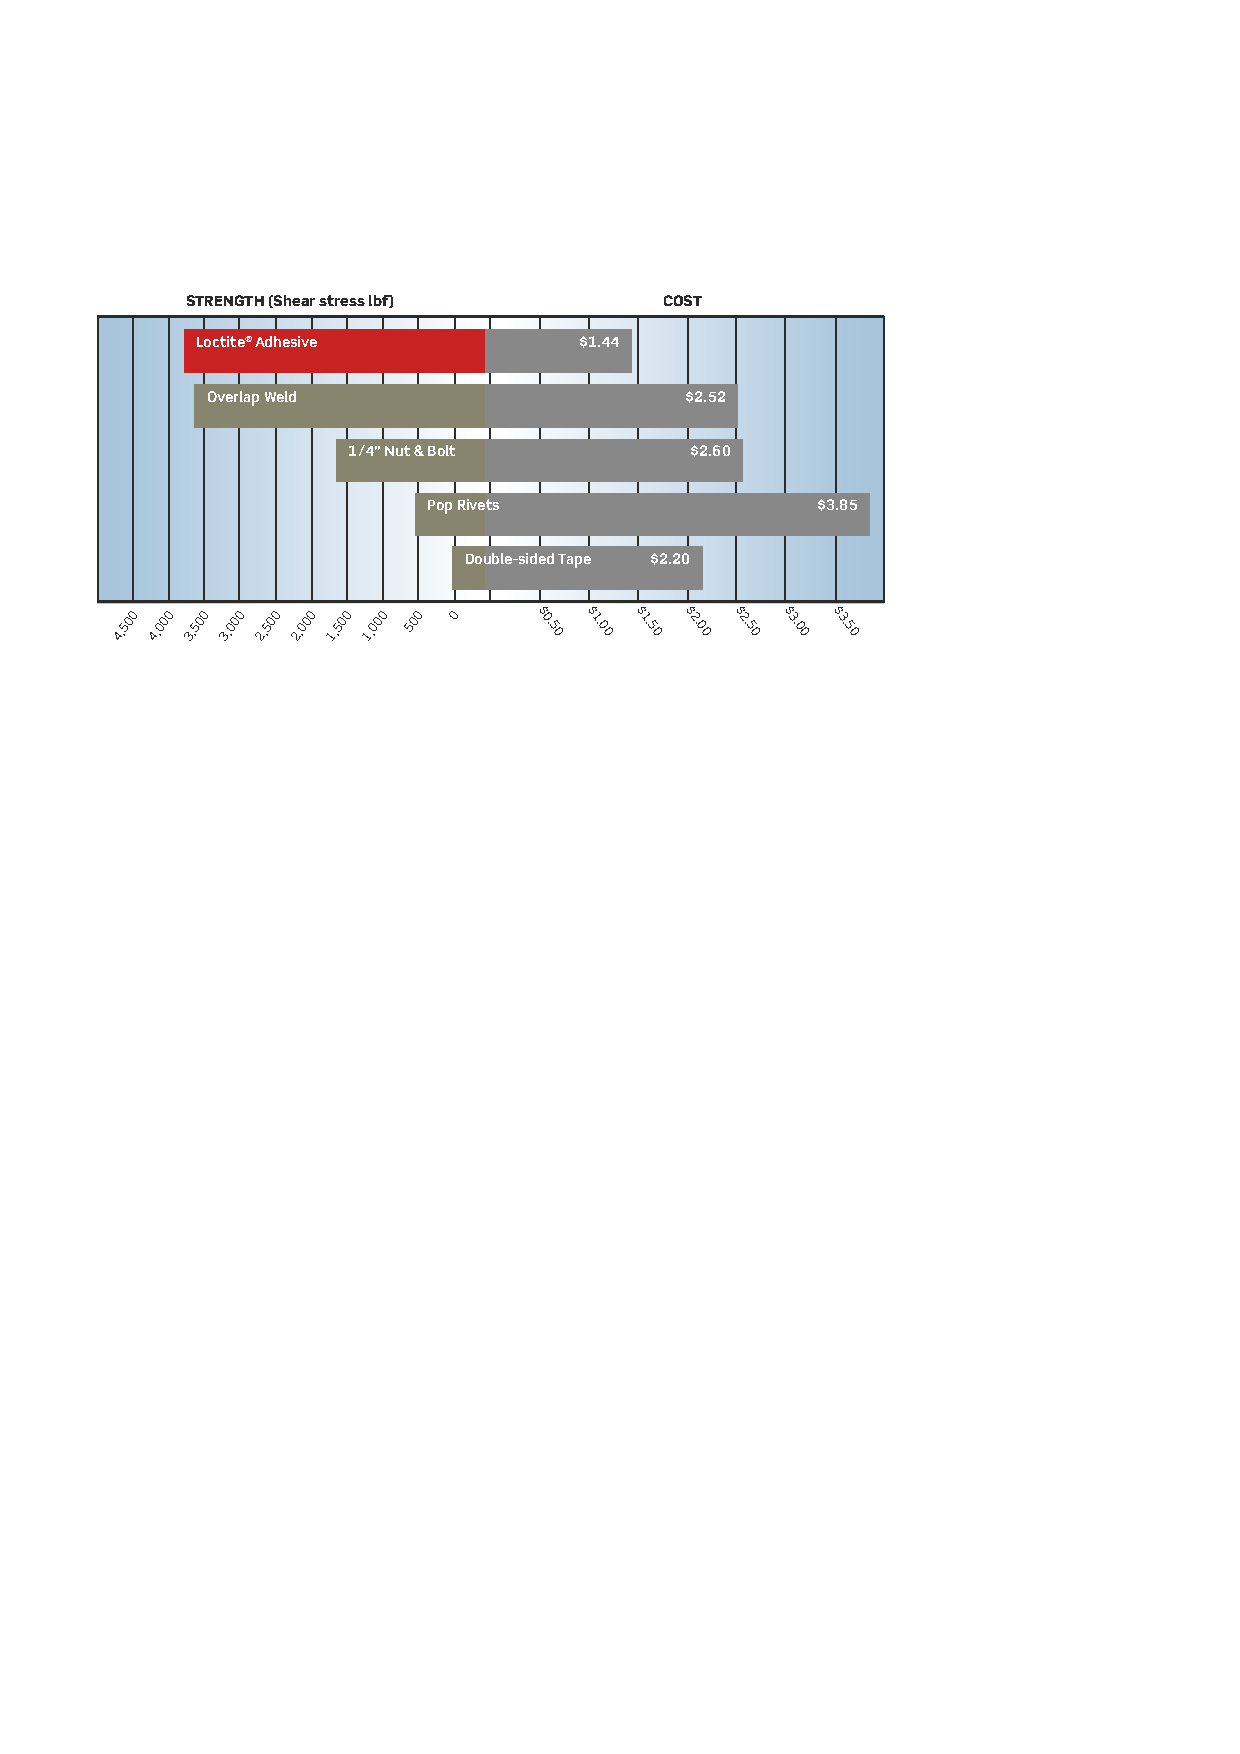
\includegraphics[width=0.7\linewidth]{./IMG_CUTRES/comparison}
	\caption[Qualitative strength and cost comparison of different joining solutions.]{Qualitative strength and cost comparison of different joining solutions. Taken from \citet{superyacht}.}
	\label{fig:comparison}
\end{figure}

As \cref{fig:comparison} illustrates, adhesives are very competitive both in bonding strength and in economical manufacturing costs \citep{superyacht}. Although other solutions, like welding, may compete in strength, adhesives are much more inexpensive than other solutions. It should be recalled that this figure only aims to give a qualitative idea of this comparison for a particular manufacturer's point of view, and should not be taken as a fact.

In order to check adhesive's suitability for their use in crashworthy elements, this study develops numerical models of adhesively bonded crash boxes subjected to impact load  using the \gls{FEM}. Information and data present in the literature are used to create and validate these models in order to ensure the accuracy of the results.

The present study aims to:

\begin{itemize}
	\item Determining an efficient adhesive modellization for its use in numerical models of adhesive joints. This modellization would also serve for studying hybrid bonding which implies the use of adhesives with other bonding solutions at the same time, such as welding or riveting.

	\item Checking the suitability of adhesives for their use in crash boxes or as a manner of improving other union types performance in that same devices.

	\item Generating a parametric model that would serve for sensitivity analysis and  optimization of the tube geometry by using the scripting capabilities of the finite element package employed.
\end{itemize}

In this introductory chapter, the most remarkable adhesive properties of interest are commented, along with experimental and numerical analysis that have been performed in the literature, with a later focus on their use in the field of crash boxes.

The present document is structured in three more chapters beyond this point, explaining the realized model, discussing the obtained results and drawing some conclusions, respectively. Two appendices are added at the end including some other aspects, such as the Python code developed for this study or the manufacturer's catalog information regarding to the selected adhesive.

\section{Adhesive characteristics}
% Resistance (general)
Advancements in the last years have improved adhesives resistant properties, making them competitive against other joining solutions for certain applications. This improvements are specially remarkable on their peel resistance ---i.e. resistance on traction loading---, which used to be one of the main obstacles for spreading their use in structural applications.

Conversely, shear resistance outstands when compared to  peeling resistance. In this case, the adhesive bonding shows performance comparable to other joining solutions. However, although loading conditions can be easily controlled in laboratory, in practical situations this may be challenging, as peel loading may appear together with shear stresses.

% ENLARGE FAILURE TYPES + IMAGES

% Fatigue
Fatigue resistance is a key feature of this type of joint, specially in certain mechanical applications, such as in structural unions in vehicles, aircrafts and machines, where vibrations suppose an important solicitation over time. They also provide certain damping \citep{Loureiro2010}, helping to insulate other components from vibrations.

% Brittleness
Adhesive unions have to be applied to larger areas ---if compared to other solutions, such as spot welding--- and, although that is not an structural property, this allows a more continuous behaviour \citep{Vaidya2006, Liao2011} by contributing to load distribution and to peak force reduction, resulting on a less brittle union on its ultimate state.

% Density
Among its non-structural properties, its reduced density contributes to create low weight unions with many different benefits, which is very interesting from both economically and environmentally points of view. Recent changes on european regulations will make low weight solutions even more important in the next years, as they will help on reducing fuel consumption and, thus, CO\textsubscript{2} and NO\textsubscript{X} emissions.

\subsection{Manufacturing process}

Adhesive manufacturing process highly differs from other joining solutions, due to the material-chemical nature of the bond, as it implies the use of one or several chemical products to cast a union based on the addition of material.

% Manufacture
The casting process also contributes on reducing brittleness: lower temperatures are required (if compared with welding) resulting in less damage to adherents’ properties, and great uniformity can be achieved in the union itself and between different unions.

Manufacture easiness also allows the creation of hybrid unions, in which the properties of one type of bonding are improved by the use of another one in addition to the former \citep{Sadowski2010, Sadowski2011}. \Cref{fig:sadowski2010_rivet_ads_improvement} shows the significant improvement on a riveted union performance when it is transformed into a hybrid one by adding an adhesive layer.

\begin{figure}
	\centering
	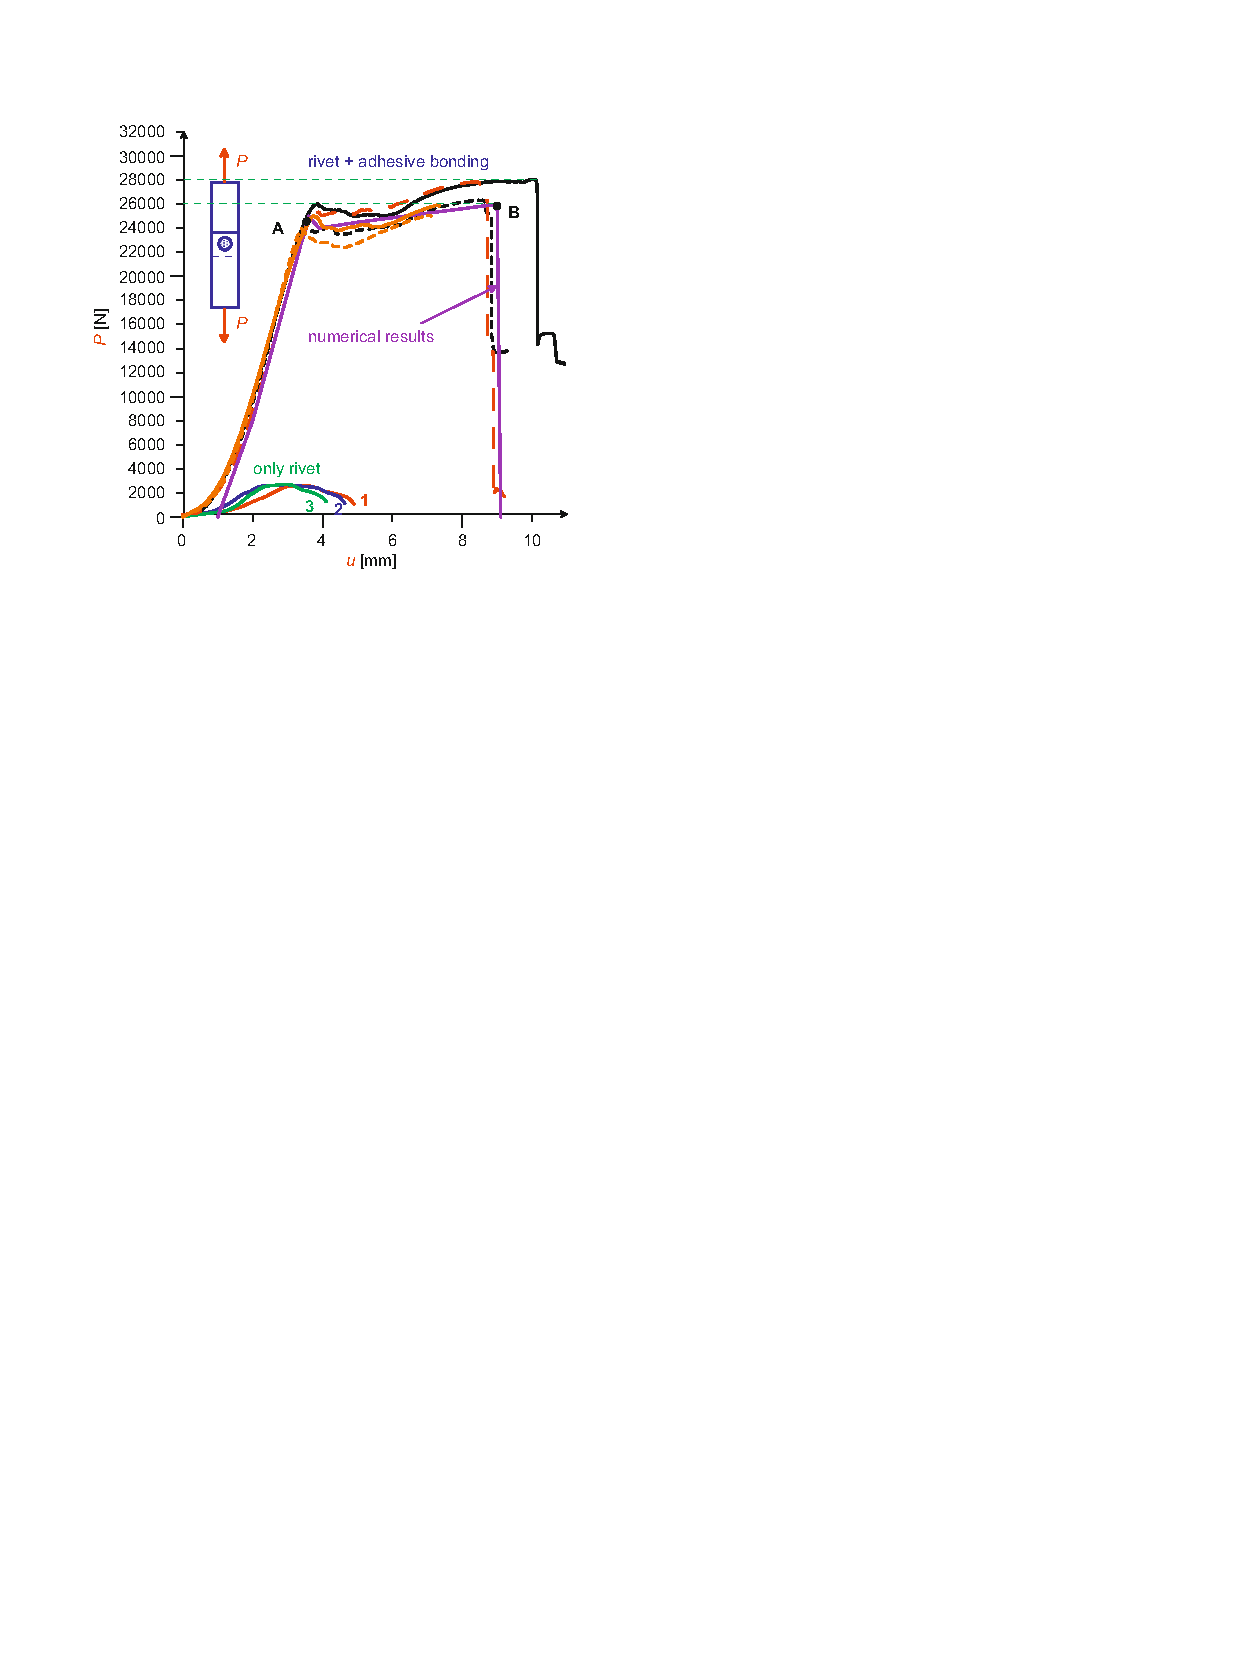
\includegraphics[width=0.65\linewidth]{IMG_CUTRES/sadowski2010_rivet_ads_improvement}
	\caption[Riveted and hybrid double lap union load-displacement up to failure comparison.]{Riveted and hybrid double lap union load-displacement up to failure comparison. Taken from \citet{Sadowski2010}.}
	\label{fig:sadowski2010_rivet_ads_improvement}
\end{figure}

A remarkable property of adhesive joints is that they also allow the creation of bonds between adherends of different nature when needed \citep{Wu2013} ---like plastic adherends, in which case it is the only bonding solution---, a feature that cannot be found on other joining solutions, such as welded unions. In spite of that, a primering treatment has to be applied to the adherends before casting the union for some adhesives. However, these bonds only need access from one side in order to be manufactured, making the joining process easier.

After that, some curing is needed. Depending on the adhesive type, the technique varies, although heat and UV curing are two of the most widespread ones, specially for monocomponent adhesives. Room temperature cure is also frequent among bicomponent adhesives. Humidity cure is another spread solution.

\subsection{Structural adhesive types}
There are different adhesives for structural applications, providing a wide range of properties adapting to different design situations, like allowing stiff and flexible bonds \citep{Loureiro2010} or the use of additives \citep{Vaidya2006}. The number of components varies between solutions, usually depending on whether they are stiff or flexible adhesives.

% Stiff adhesives
Epoxy based adhesives are one of the main types of stiff adhesives used for structural bonding. They are easy to cast, as they are monocomponent, although they require curation processes, which imply heating and time. There are other stiff solutions as bicomponent adhesives. These bicomponent adhesives are usually manufactured from the mixture of a pre-polymer with the corresponding catalyst.

Examples of stiff adhesives include Loctite Hysol 9514 \citep{manufCatalog} (epoxi, monocomponent), SikaPower 2910 (isocianate polymer, bicomponent), or Araldite AV318 with hardener HV998 (epoxi, bicomponent).

% Flexible
On the other hand, flexible solutions are usually bicomponent, made of polyurethane or sylicone. Their mechanical properties usually provide additional damping to other components, but they are not usually suitable for working on high temperature scenarios, as their strength rapidly suffers big drops (see \cref{fig:loctite_hysol_temp_dependency}). Some examples of these flexible adhesives include Loctite Hysol 9480 (epoxi, bicomponent), or SikaFlex 256 (polyurethane, monocomponent).

\begin{figure}
	\centering
	\begin{minipage}[b]{.48\linewidth}
		\centering
		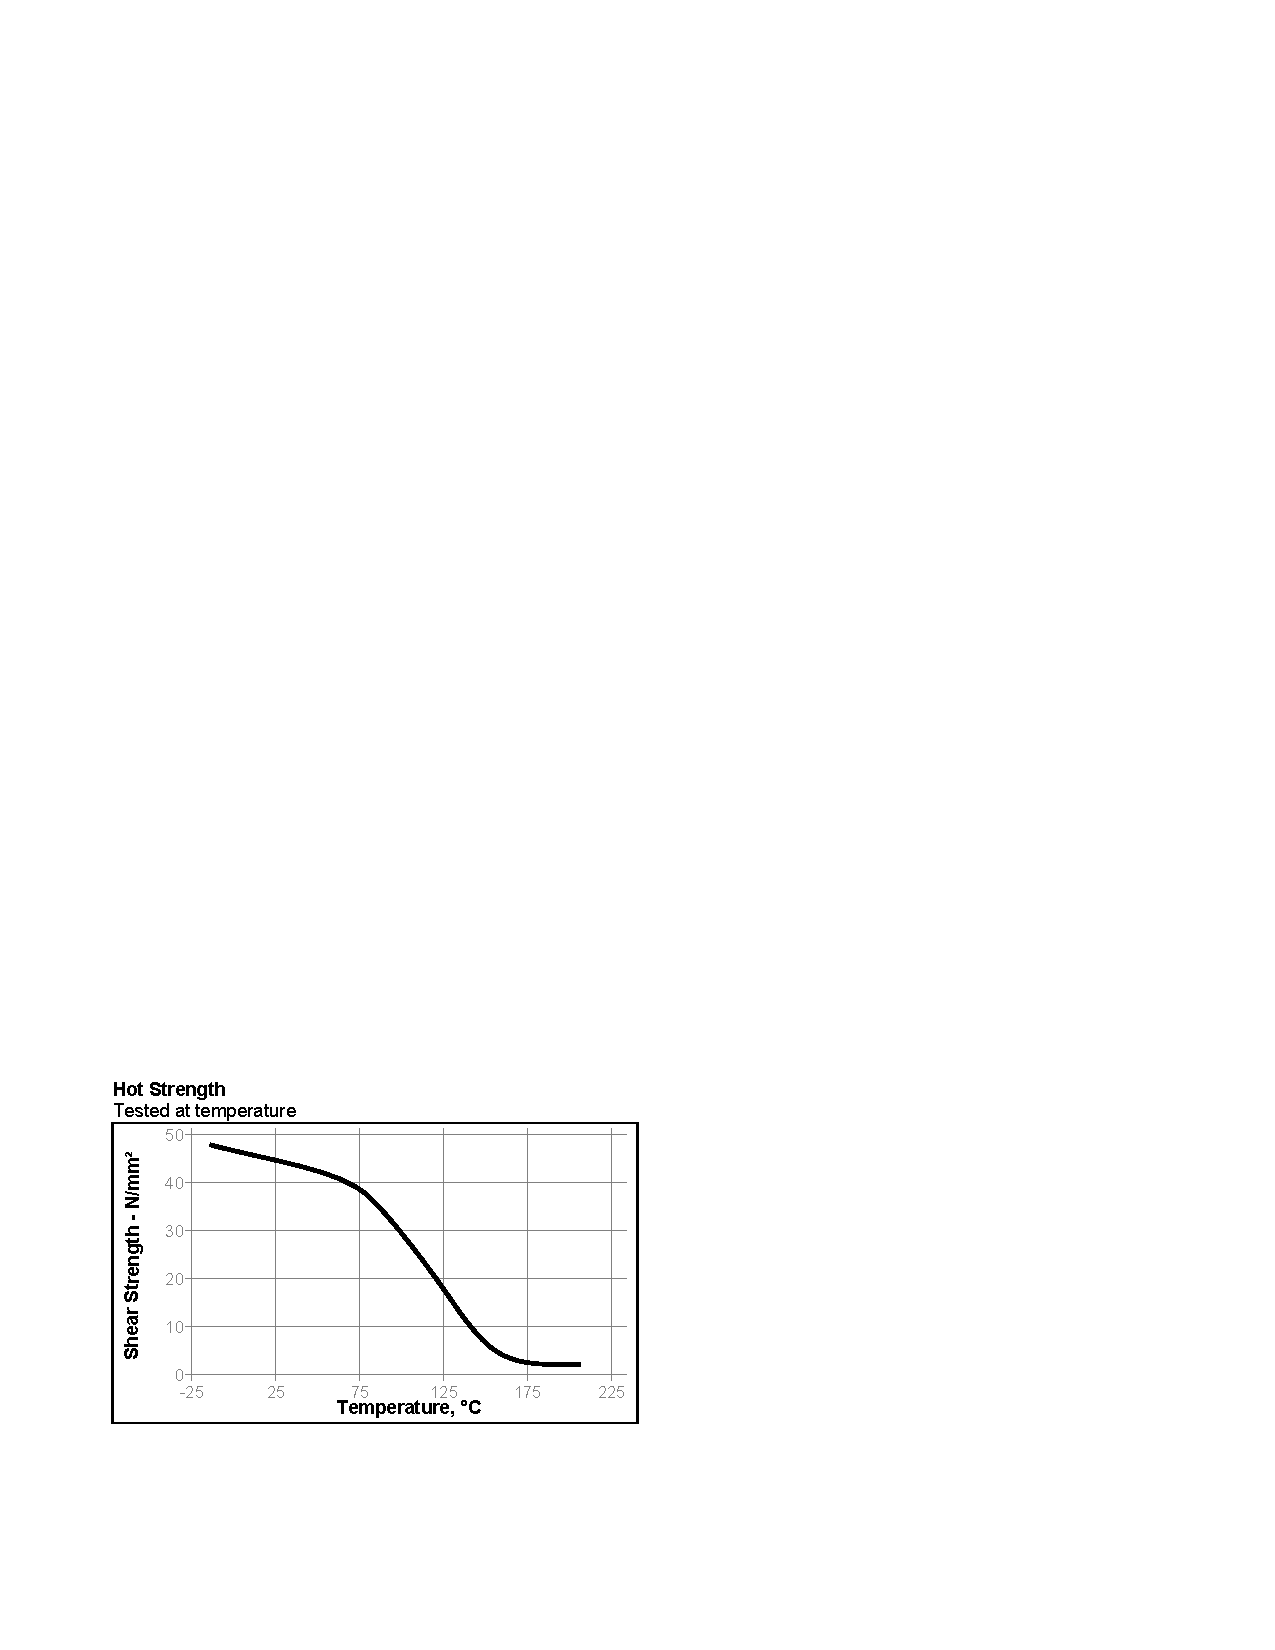
\includegraphics[width=\linewidth]{IMG_CUTRES/loctite_hysol_9514_temp_dependency}
	\end{minipage}
	\quad
	\begin{minipage}[b]{.48\linewidth}
		\centering
		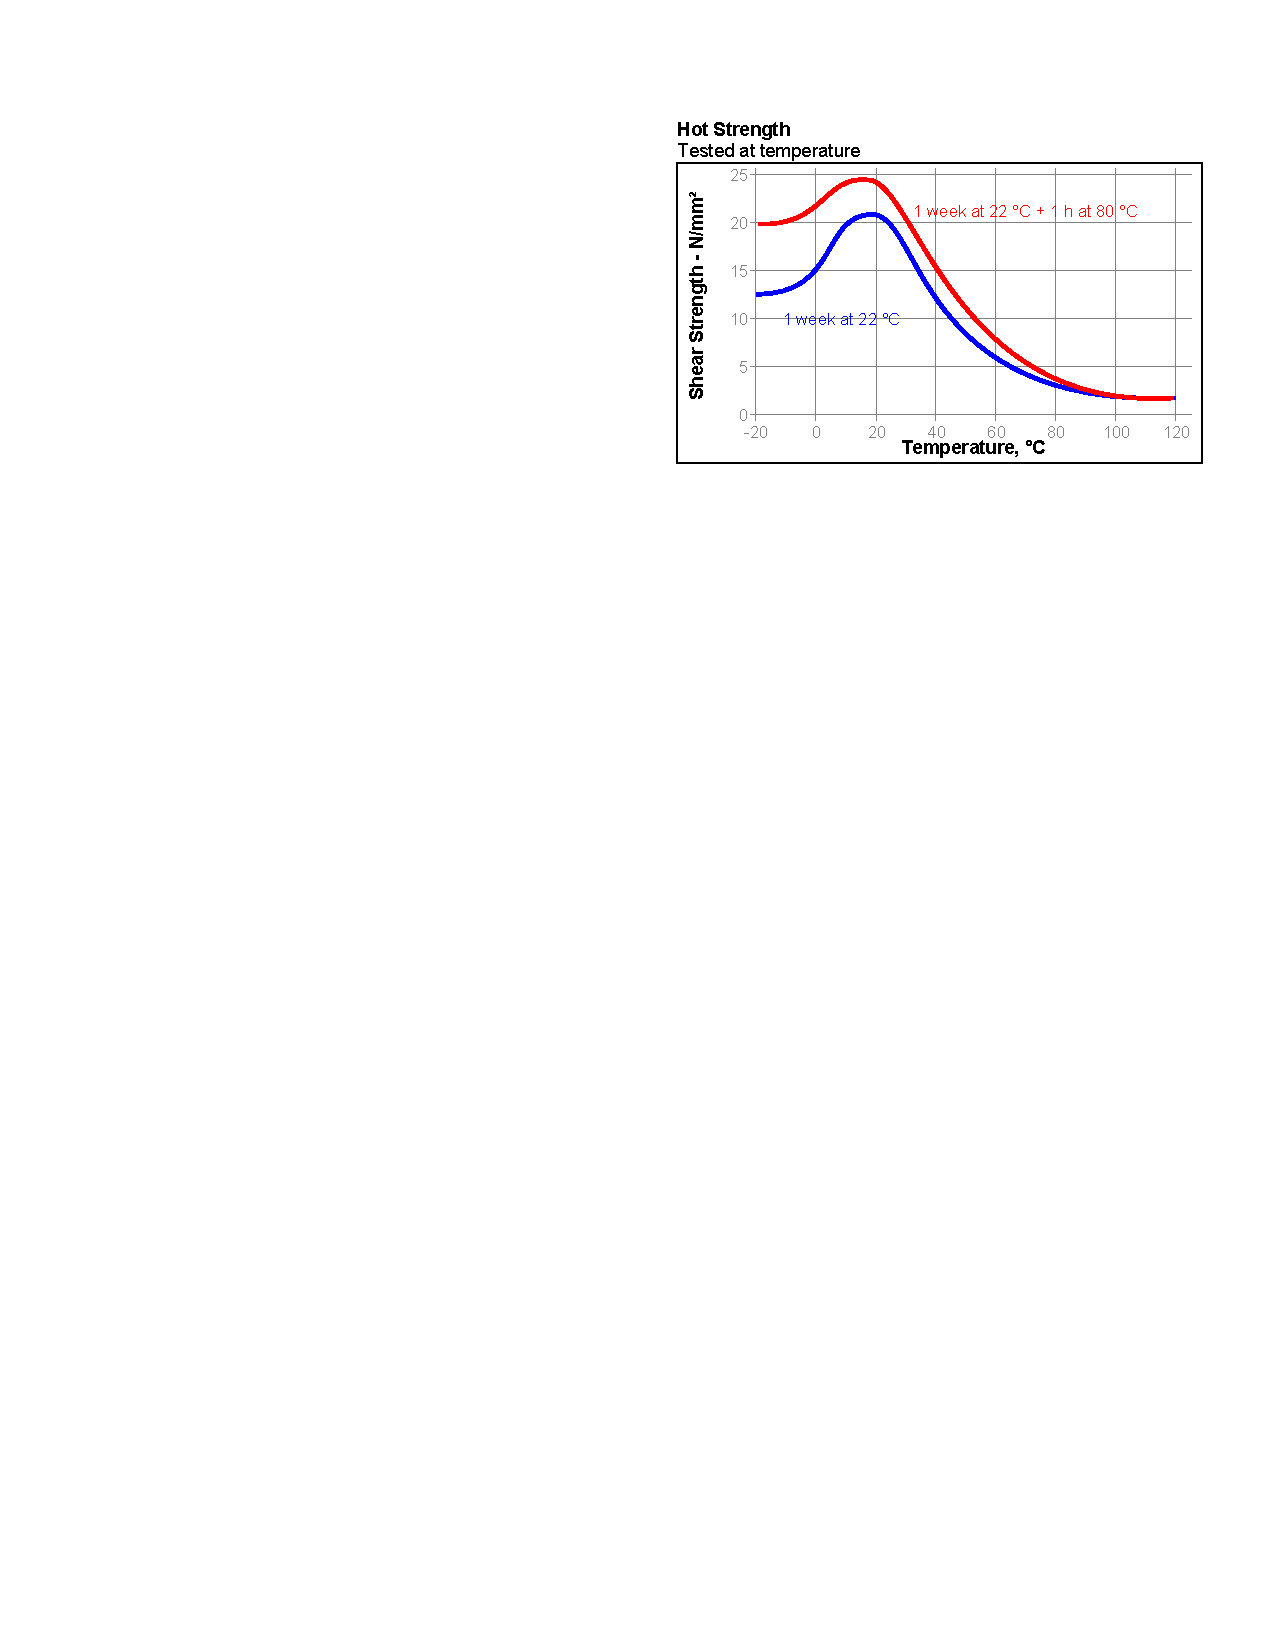
\includegraphics[width=\linewidth]{IMG_CUTRES/loctite_hysol_9480_temp_dependency}
	\end{minipage}
	\caption[Shear strength dependency of temperature for a stiff adhesive (Loctite Hysol 9514, left) and for a flexible adhesive (Loctite Hysol 9480, right)]{Shear strength dependency of temperature for a stiff adhesive (Loctite Hysol 9514, left) and for a flexible adhesive (Loctite Hysol 9480, right). Taken from \citet{manufCatalog}.}
	\label{fig:loctite_hysol_temp_dependency}
\end{figure}

% Adhesive tape
Finally, adhesive tape appears as some sort of ``pre-cast'' bonding solution, with a much simpler casting process, although their behaviour has not been as widely tested as other solutions \citep{Kadioglu2014}. 3M products are the most used for this application, including 3M SBT 9245 and the 3M VHB product series.

Due to the mentioned properties ---but specially their resistance and low-weight---, adhesives have become a widely used bonding solution in the aerospace industry: in fuselage structure, in aircraft wings stiffener ribs, etc. It is also becoming an appealing bonding solution in other fields, such as in the automotive industry \citep{Wu2006, Greve2007, Grant2009, Scattina2011, Kadioglu2014, SernaMoreno2015}, where their use is spreading every moment. Even other industries like the yachting one \citep{superyacht} are starting to implement this technology thanks to the adhesive durability, environmental impact, strength and manufacturing costs.

\section{Structural adhesives for energy absorption devices}
In the automotive industry, one of the latest applications of adhesives is their use in crash box design, and it is the focus of this study. Crash boxes belong to the pasive safety measures installed on a vehicle. Pasive safety refers to minimizing damage to the occupants during an accident, being active safety a set of measures that aim to prevent the event itself.

% Introd to adhesive crash box
These devices are installed as a part of the vehicle's structure, usually just behind the bumper, being their function to absorb the most in case of impact on an accident. As an example, the precise location of these elements in a 2011 Audi A8 is showed in \cref{fig:audiA8struc}, and detailed in \cref{fig:audiA8detail}. In the general view, different materials are highlighted, illustrating how adhesives can be interesting in this industry.

\begin{figure}
	\centering
	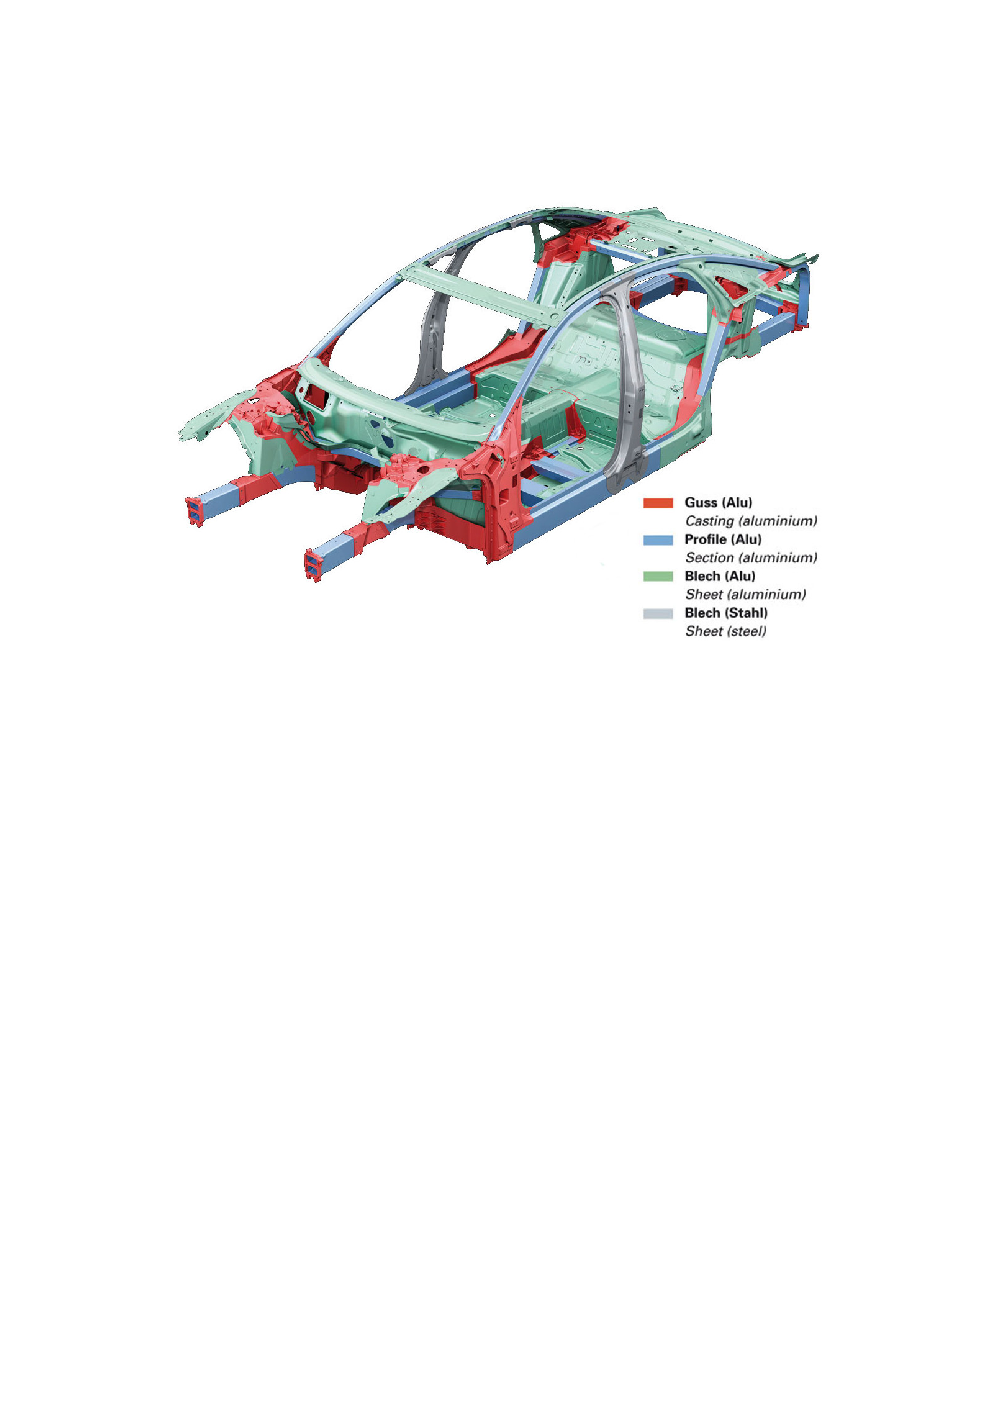
\includegraphics[width=0.65\linewidth]{IMG_CUTRES/audiA8struc}
	\caption[Body structure of a 2011 Audi A8.]{Body structure of a 2011 Audi A8. Taken from \citep{audiA8}.}
	\label{fig:audiA8struc}
\end{figure}

\begin{figure}
	\centering
	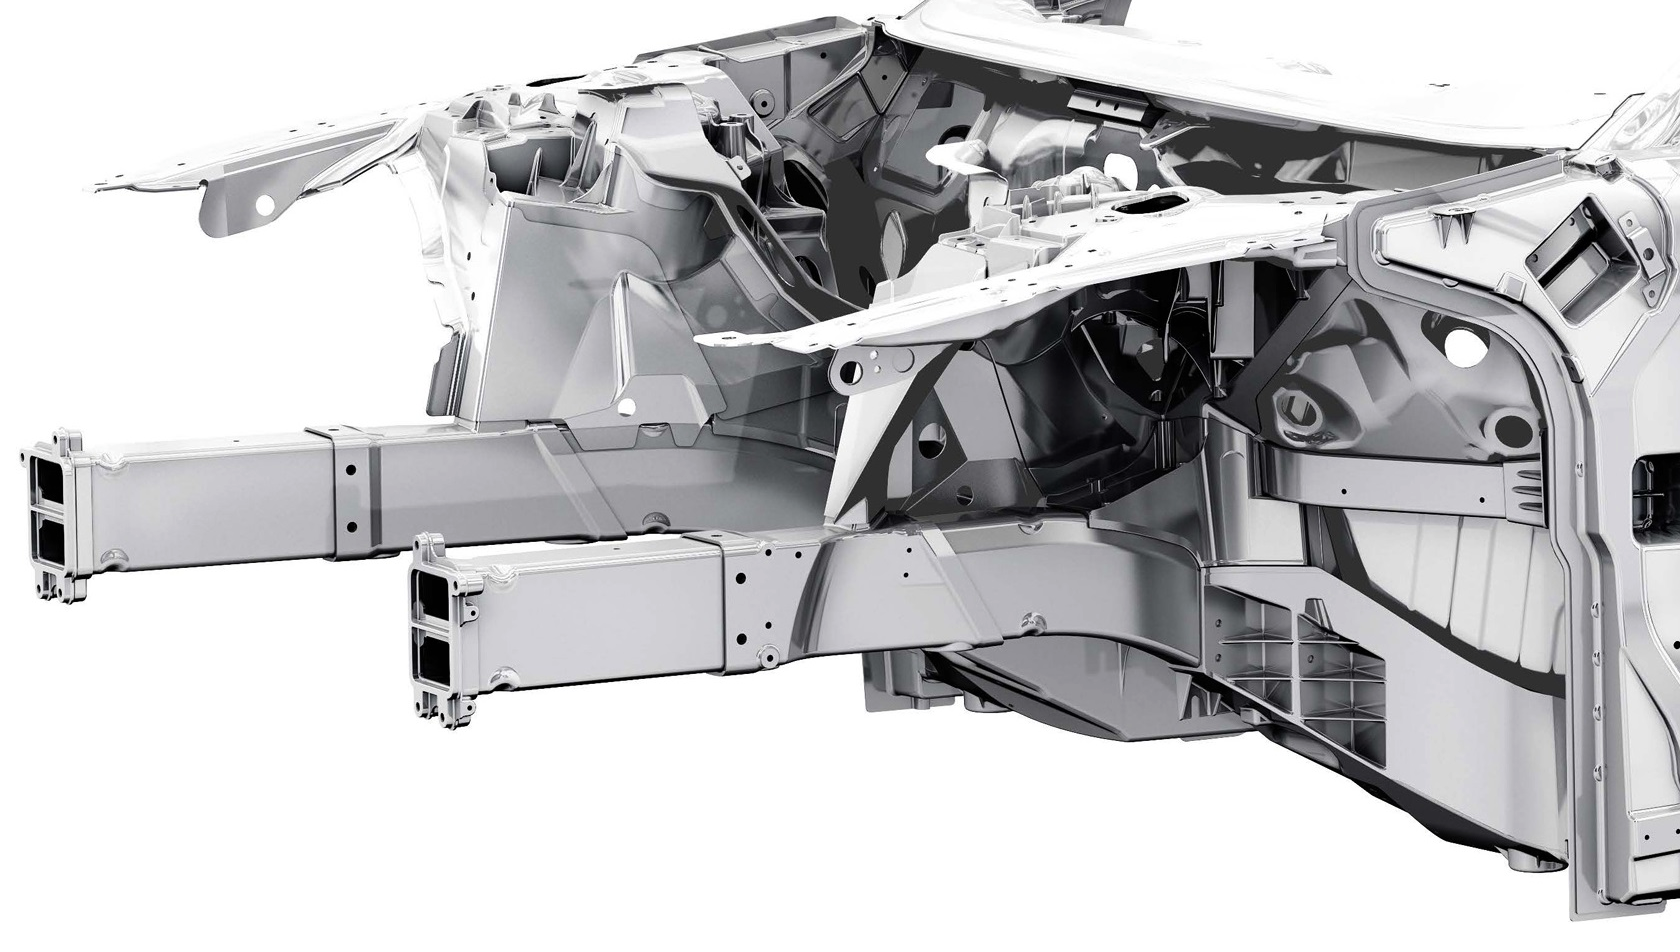
\includegraphics[width=0.7\linewidth]{IMG_CUTRES/audiA8detail}
	\caption[Detail of energy absorption devices in the front of a 2011 Audi A8.]{Detail of energy absorption devices in the front of a 2011 Audi A8. In this case, an aluminum tube with two cavities was used. Taken from \citep{audi}.}
	\label{fig:audiA8detail}
\end{figure}

% Design variables
As \citet{Hou2008} pointed out, the design of a crashworthy element pursues to maximize \gls{Ea} through elastic and plastic deformation \citep{Wu2006}, but this also increases the transmitted peak force, which is the greatest transmited force value within the crash time span and it is considered one of the main reasons of biomechanical injury. \Gls{SEA} has been used as parameter by some authors \citep{Lee2006, Peroni2009, Scattina2011} for measuring the element's effectiveness on absorbing energy, rather than the total \gls{Ea}. \Gls{SEA} can be obtained by dividing \gls{Ea} by the total mass of the crash box \citep{Lee2006, Peroni2009, Scattina2011}.  A compromise between \gls{Ea} ---or \gls{SEA} on its place--- and \gls{Pk} has to be achieved. Weight is another variable usually taken into account. \Cref{fig:f-d} represents a common \gls{F-D} resultant of a crash test; on it, the first peak corresponding to \gls{Pk} can be seen, together with \gls{Ea}, depicted as $E$.

\begin{figure}
	\centering
	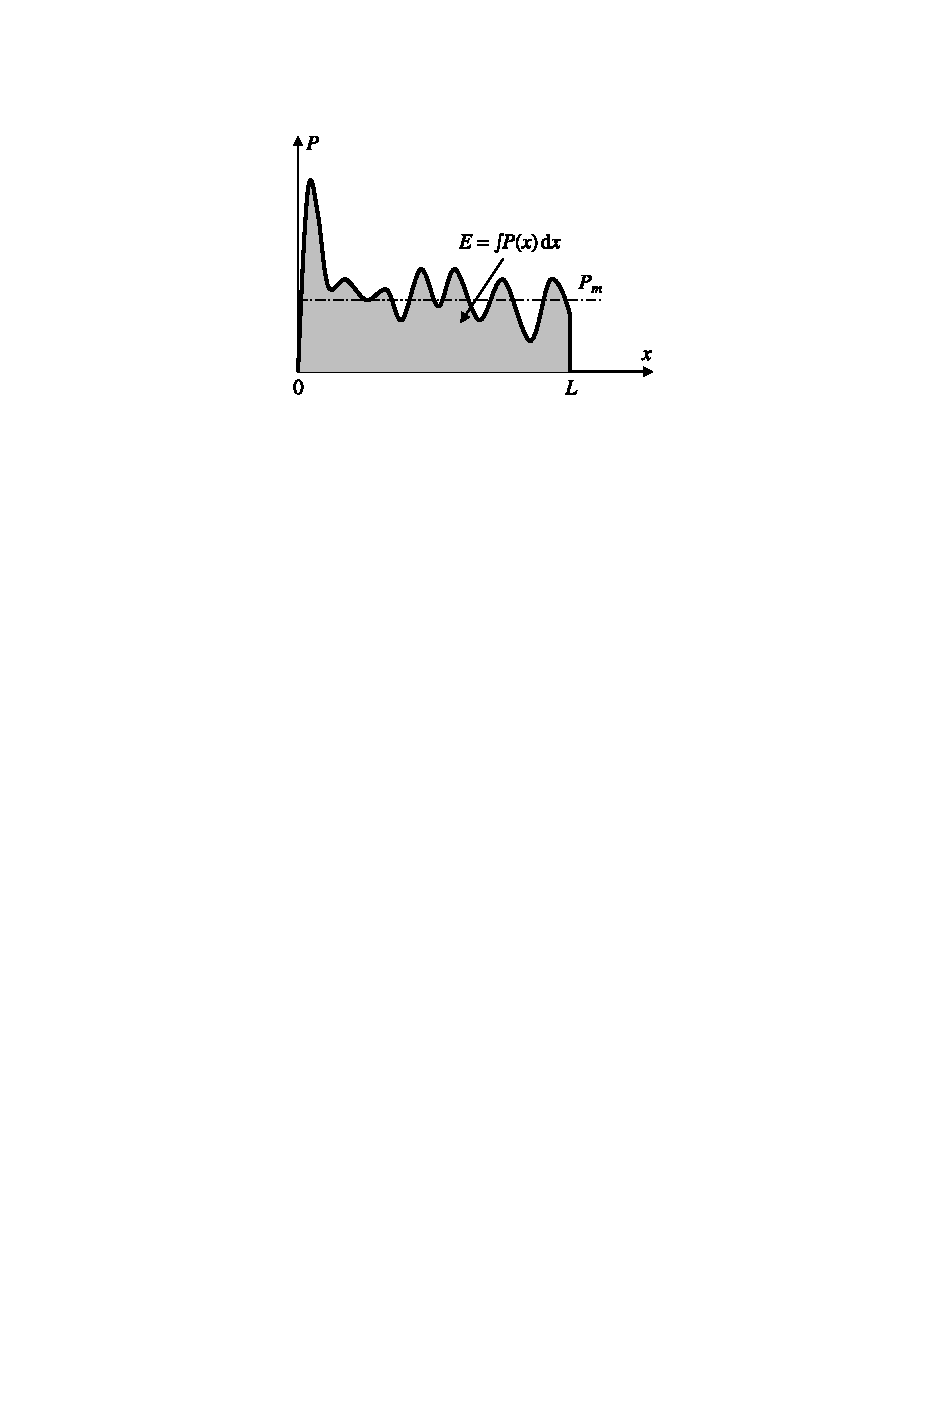
\includegraphics[width=0.7\linewidth]{IMG_CUTRES/f-d}
	\caption[Typical \acrlong{F-D} in a crash test.]{Typical \acrlong{F-D} in a crash test. Taken from \citet{Scattina2011}.}
	\label{fig:f-d}
\end{figure}

\section{Experimental analysis on adhesives}

Experimental studies mainly aim to deduce adhesive parameters by testing normalized joints or they check their performance on bigger models that include whole devices, such as crash boxes.

\citet{Lee2006} showed the adhesive's better performance as a bonding solution if compared to spot welding in terms of \gls{SEA}. These two bonding methods were also tested, together with laser weld, by \citet{Peroni2009}, who also included different box section geometries in their studies.

On impact, a Charpy-like pendulum has been used to test adhesive behaviour \citep{Goglio2008, Kadioglu2014}. It was concluded that maximum strength of the adhesive maintains its value when comparing to static results \citep{Goglio2008}. \citet{Kadioglu2014} tested adhesive tape and found that results vary very little with impact speed.

\subsection{\Acrlong{SLJ} and peel test}
% DIVIDE AND ENLARGE

Although different tests were proposed \citep{Kihara2003, Raykhere2010} in order to obtain adhesive's properties on peel and shear loading, \acrfull{SLJ} and peel test remain as the most extended experiments to obtain shear and traction stiffness and strength of different bonding solutions.

Several authors have tried variations on these tests in order to check the influence of different parameters, such as the adhesive layer thickness and overlap length \citep{Liao2011}, including fillets on the bonding edges \citep{Grant2009}, or even the use of certain additives for the adhesive itself \citep{Vaidya2006}.

\citet{Loureiro2010} presented a very complete study of stiff and flexible adhesive's properties, in which they tested \acrlong{SLJ} and T-joints analyzing its mechanical behaviour on static, impact and fatigue loads, apart from damping measurement.

They found that stiff adhesives had a bigger impact failure load than their counterpart, although they are comparable. In single lap joints, stiff adhesives produced adherend yielding, which was the cause of the failure load increase. Flexible adhesives showed a bigger distribution in time of load and adherend yielding in T-joints.

\subsection{Fatigue and damping}
\citet{Loureiro2010} found that stiff and flexible adhesives have very similar damping ratios, in spite of expecting higher values on the flexible one. They calculated the damping ratios by determining the natural frequency of each performed test as a whole through the bandwidth method. Then, the union damping could be deduced. The results varied approximatedly between $0.25\%$ and $0.30\%$, depending on the test from which it was deduced.

On fatigue, \citet{Loureiro2010} also found many similarities between the stiff and the flexible adhesives, as it can be seen on \cref{fig:Loureiro_fatigue}, depicting cohesive failure in all the performed tests. Heating during the test could be the reason of this similarity, as the flexible solution was expected \textit{a priori} to show better results.

\begin{figure}
	\centering
	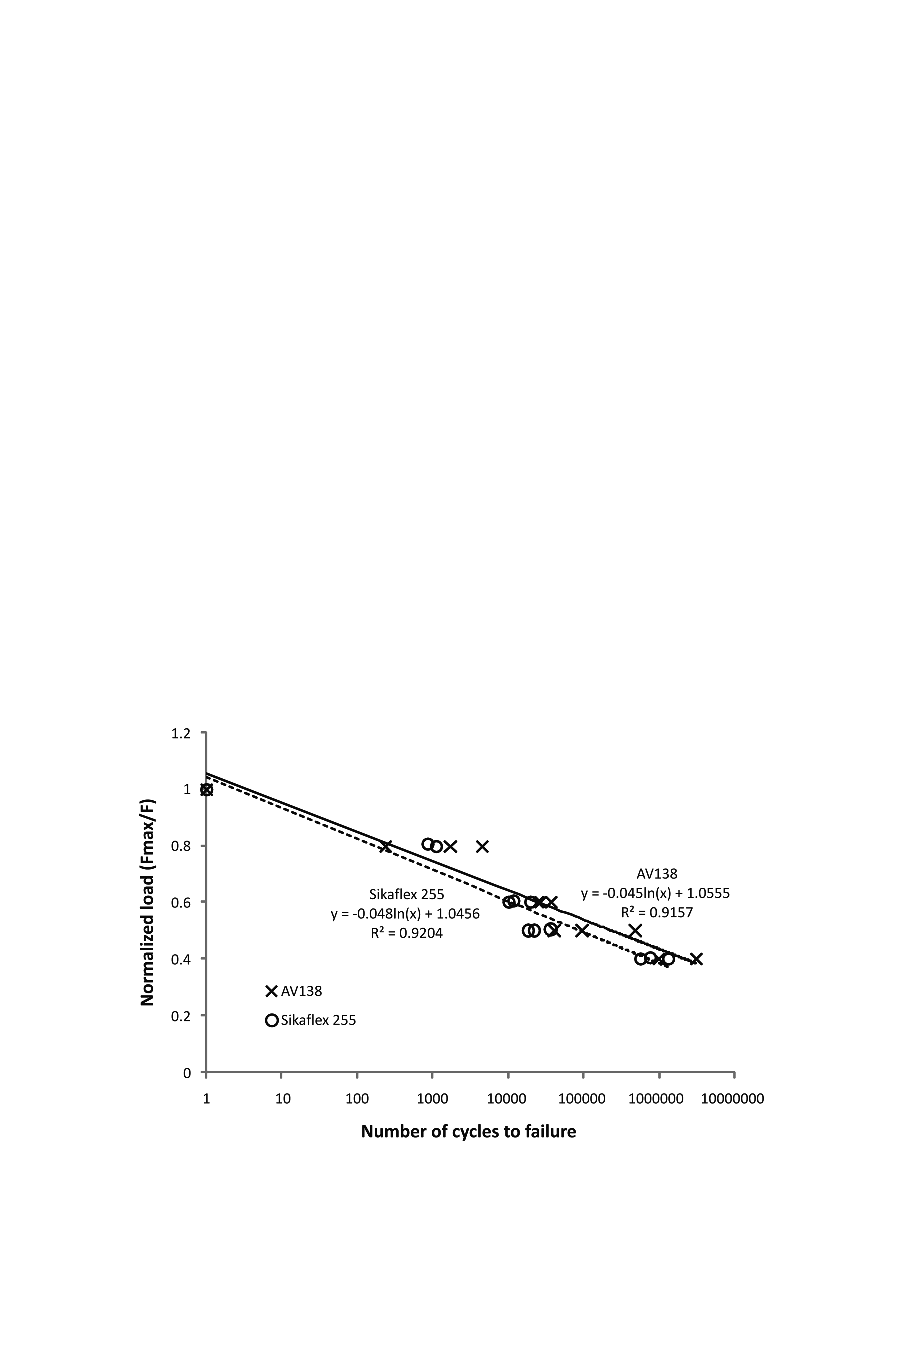
\includegraphics[width=0.7\linewidth]{IMG_CUTRES/Loureiro_fatigue}
	\caption{Results of the fatigue tests carried out by \citet{Loureiro2010} on \gls{SLJ} bonded with AV138 and Sikaflex 255 adhesives.}
	\label{fig:Loureiro_fatigue}
\end{figure}

\section{Numerical modeling of adhesives}

Publications about numerical modeling of adhesives analyze details that are difficult to measure on experiments ---such as a more precise stress distribution within the union---, and also the modellization of entire devices like in the experimental testing. However, unlike the experimental testing, modelling lacks of certain approaches in the literature, or their presence is scarce, such as damping and fatigue.

Adhesive bonding behaviour has been widely modelled for a structural use, usually as a previous phase to laboratory experiences \citep{Sato2000, Grant2009, Loureiro2010, Yang2012, Sadowski2014}, which usually included \glspl{SLJ} and peel tests.

The \gls{SLJ} test has also been modelled \citep{Vaidya2006}, as a way of obtaining its parameters for the used formulation \citep{Scattina2011}. Analogously, some authors used \glspl{SLJ} and T-joints as a validation for their models \citep{Loureiro2010, Liao2011}. \Gls{SLJ} modelling allows many different studies:
\begin{itemize}
	\item Stress distribution over the bonded surface: this was the main focus of the study carried out by \citet{Vaidya2006, Liao2011, Hazimeh2014} with different focuses each, finding a great uniformity if compared to other bonding solutions and highlighting the mostly stressed regions, which would help in reinforcements design if needed. \citet{diaz2010benchmarking} published a study aimed to compare the performance of several modelizations with different element types of a joint made of CFRP adherends bonded by  epoxy  adhesive.

	On the other hand, \citet{Vaidya2006} tested two different adhesives and a modification on one of those, after experimentally obtaining the corresponding parameters. They highlighted the stress distribution over the union surface. \citet{Liao2011} meanwhile studied the stress distribution along different paths within the bonded surface on static and impact loading. Finally, \citet{Hazimeh2014} made an analysis of the influence of different parameters such as union length and width or adhesive and adherend thickness, among others.

	\item Comparison with other tests: like tapered lap and scarf joints modelled by \citet{Sato2000}, as depicted in \cref{fig:sato_joints}. They concluded that tapered lap joints worked better than \gls{SLJ} on reducing stress concentration, and that scarf joints worked better than those both, in spite of their obvious additional manufacture difficulties.

	Meanwhile, \citet{Grant2009} did the proper modifications on the adhesive by adding fillets at the bonding end, instead of a square end, finding a resistance improvement on tension. Other non-canonical tests were also modelled, like \citet{Kihara2003} did in 2D for impact loading.

	\begin{figure}
		\centering
		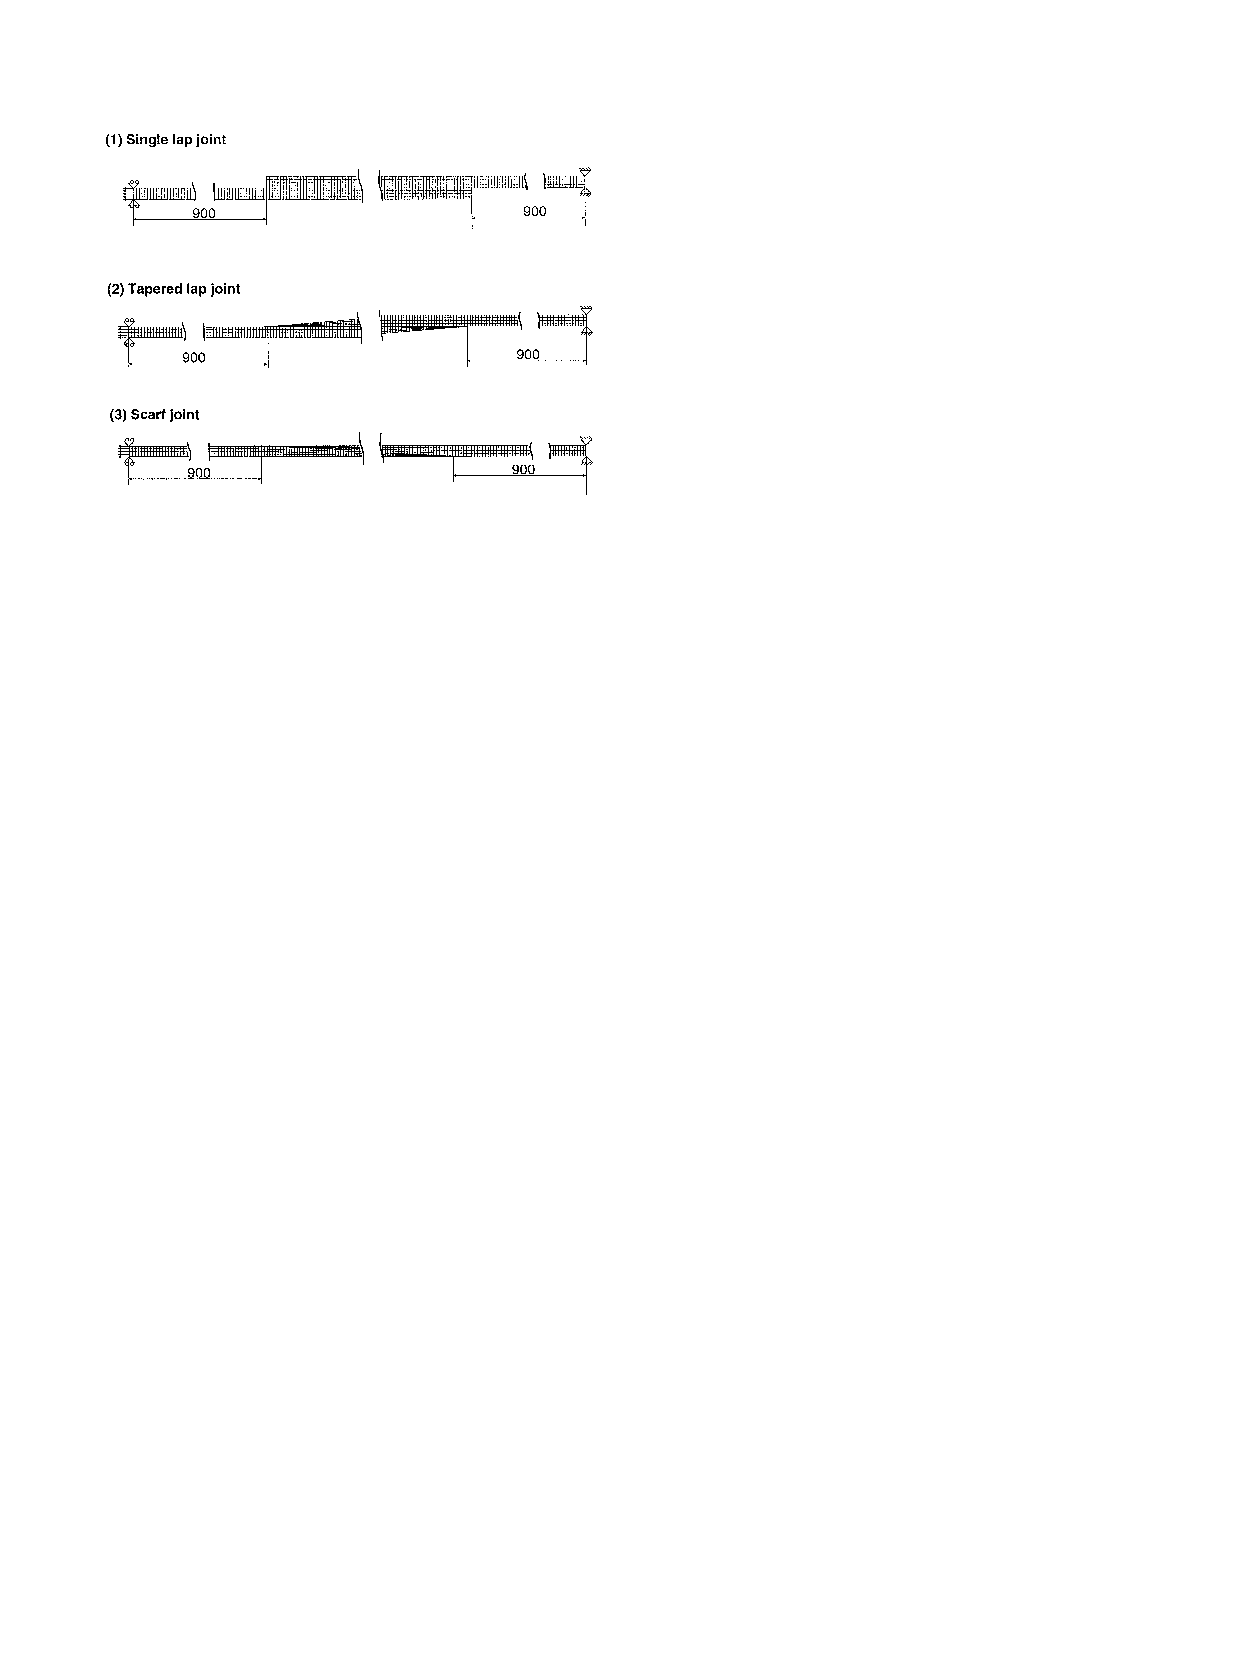
\includegraphics[width=0.7\linewidth]{IMG_CUTRES/sato_joints}
		\caption[Single lap, tapered and scarf joints.]{Single lap, tapered and scarf joints. Taken from \citet{Sato2000}.}
		\label{fig:sato_joints}
	\end{figure}

	\item Comparison with other bonding solutions: such as rivets and hybrid unions of rivets and adhesives, which were studied in detail by \citet{Sadowski2010, Sadowski2011, Sadowski2014} (see \cref{fig:sadowski_riv}), concluding that adhesives highly improve other union types performance when casted together, as it was pointed in \cref{fig:sadowski2010_rivet_ads_improvement}. They made models at different scales, and eventually tested crash boxes with hybrid bonds.

	\begin{figure}
		\centering
		\begin{minipage}[b]{.2\linewidth}
			\centering
			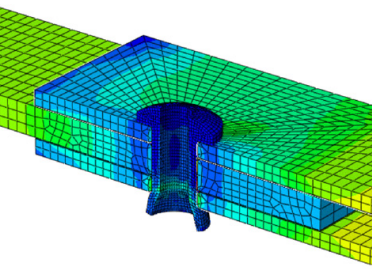
\includegraphics[width=\linewidth]{IMG_CUTRES/sadowski_riv1}
		\end{minipage}
		\quad
		\begin{minipage}[b]{.2\linewidth}
			\centering
			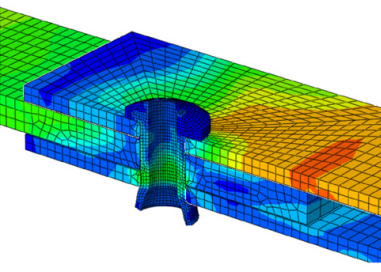
\includegraphics[width=\linewidth]{IMG_CUTRES/sadowski_riv2}
		\end{minipage}
		\quad
		\begin{minipage}[b]{.2\linewidth}
			\centering
			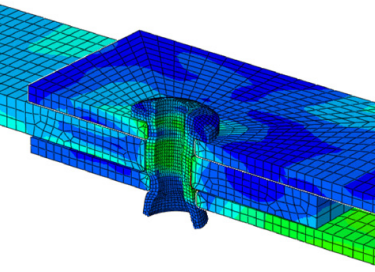
\includegraphics[width=\linewidth]{IMG_CUTRES/sadowski_riv3}
		\end{minipage}
		\quad
		\begin{minipage}[b]{.2\linewidth}
			\centering
			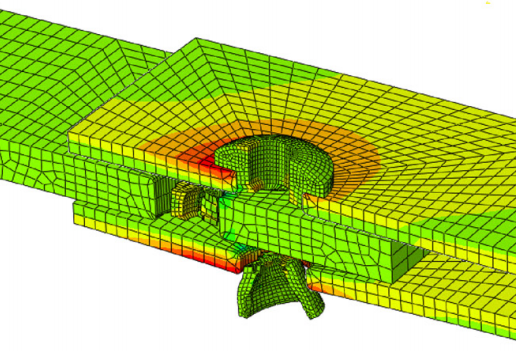
\includegraphics[width=\linewidth]{IMG_CUTRES/sadowski_riv4}
		\end{minipage}
		\caption[Double lap joint test of a hybrid union of rivets improved with adhesives.]{Double lap joint model of a hybrid union of rivets improved with adhesives. Taken from \citet{Sadowski2010}}
		\label{fig:sadowski_riv}
	\end{figure}

\end{itemize}

In spite of having been modelled for long time, the adhesive behaviour formulation was not clear until recently. During the development of the formulation used nowadays, other models have been used, including: three and five elements Voigt viscoelastic models \citep{Sato2000}; isotropic elastic-plastic material with kinematic hardening \citep{Vaidya2006}; and even a highly specific formulation for this bonding system \citep{Greve2007}. Adhesives are nowadays modelled as linear elastic isotropic materials with damage models, and the currently used model for adhesive delamination was formulated by \citet{Alfano2001}.

Eventually, formulation development lead to modelling of entire crash boxes \citep{Scattina2011, Yang2012, Yamashita2013}. \citet{Scattina2011} studied crash boxes previously tested by \citet{Peroni2009}. They obtained some adhesive parameters for their numerical input and validating the made models. \citet{Yang2012} made an analogous work for obtaining the adhesive properties and modelled a hexagonal crash box.

Eventually, modelling also allows a certain optimization process. \citet{Hou2008} tried this on several multi-cell square crash boxes on impact loading.

In relation to modelling software, Abaqus ---made by Dassault Systèmes--- and LS-DYNA ---by Livermore Software Technology Corporation--- are the two most commonly used conventional software packages used for this purpouse, having validated formulations. Abaqus is the chosen one for this study and in the next chapter the numerical model developed within Abaqus framework will be described.

\chapter{Numerical model of an adhesively bonded crash box}
\label{model}

The modelled crash box consists of two adherend plates made of steel that create a tube of square section by being bonded together with adhesive. The union is practiced on the surface of two flanges on each adherend side. Adhesive failure and adherend plastification are taken into account.

The tube is crushed between two rigid plates, one fixed and the other moving at impact speed. In order to ease the formation of a stable collapse mechanism, triggering is applied on a certain section near the frontal end of the tube. The trigger consists on a small change on a particular zone of the tube in order to provoke the initiation of a desired local collapse in that zone, aiming to lead to a certain global collapse mechanism; examples include indentations or holes near the head end. In addition, some models count with rivets to avoid certain unstable failures.

\section{Geometry}

In order to ease model comparation and validation, the crash box geometry was created to reflect those tested by \citet{Peroni2009} and later modelled by \citet{Scattina2011}.

Among the five different square section layouts tested by \citet{Peroni2009}, the following two sections, depicted in \cref{fig:tubes}, were modelled in the present study:
\begin{itemize}
	\item Double hat section \citep{Lee2006, Yang2012, Yamashita2013}.
	\item Top-hat \citep{Scattina2011, Yamashita2013}.
	%\item Asymetric mid-sides bonding.
\end{itemize}

\begin{figure}
	\centering
	\begin{minipage}[b]{.45\columnwidth}
		\centering
		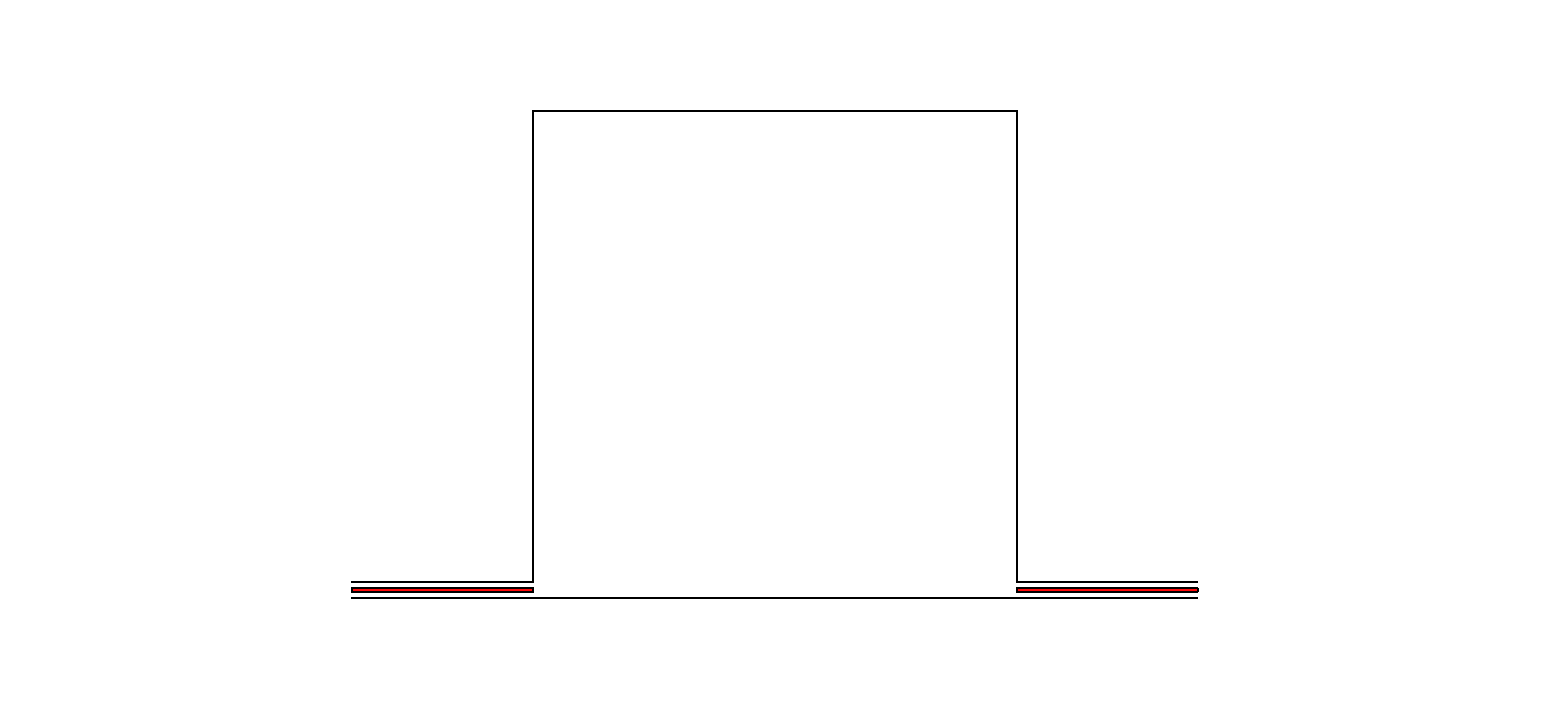
\includegraphics[height=42mm]{IMG_CUTRES/A_section}
	\end{minipage}
	\hfill
	\begin{minipage}[b]{.45\columnwidth}
		\centering
		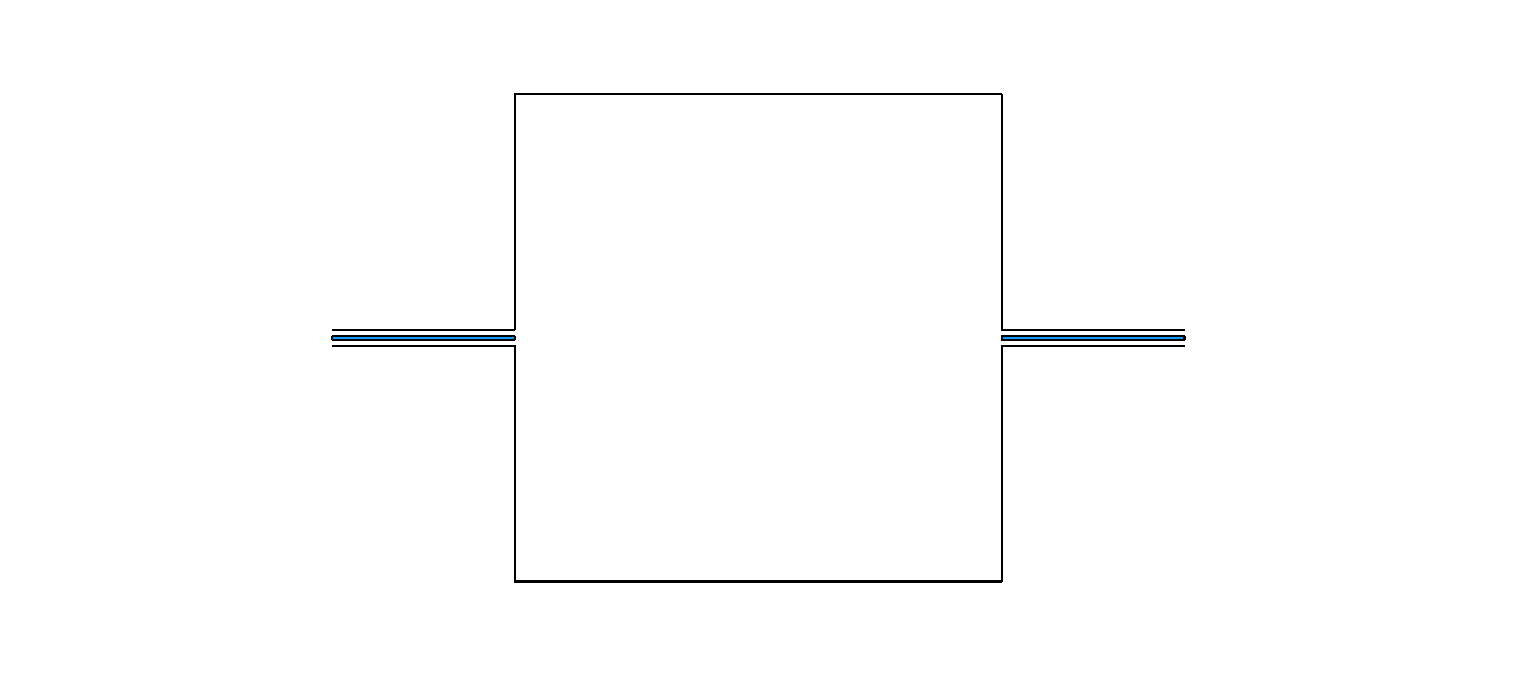
\includegraphics[height=42mm]{IMG_CUTRES/B_section}
	\end{minipage}
\\[10mm]
\begin{minipage}[b]{.4\linewidth}
	\centering
	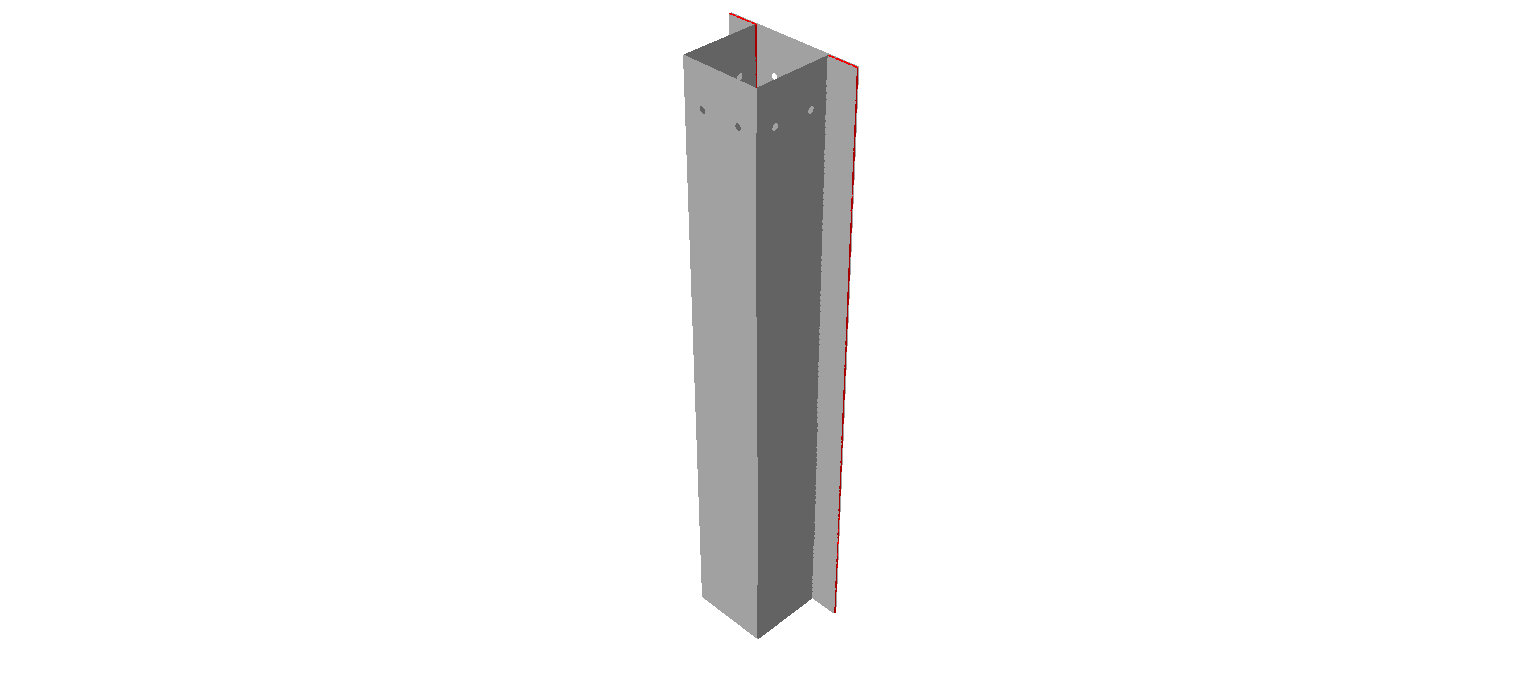
\includegraphics[height=135mm]{IMG_CUTRES/A_tube}
\end{minipage}
\hfill
\begin{minipage}[b]{.4\linewidth}
	\centering
	
\includegraphics[height=135mm]{IMG_CUTRES/B_tube}
\end{minipage}

	\caption[Modelled tubes and corresponding cross sections.]{Modelled tubes and corresponding cross sections. Top-hat section with adhesive in red (left), and double hat section with adhesive in blue (right).}
	\label{fig:tubes}
\end{figure}

These sections allow comparison between cross sections as each case has the same box perimeter and the same bonding surface \citep{Peroni2009}. In addition, two of the union layouts tested by \citet{Peroni2009} were discarded due to serious bond casting difficulties. Measures of three of the tubes tested by these authors are depicted in \cref{fig:crash_box}.

\begin{figure}
	\centering
	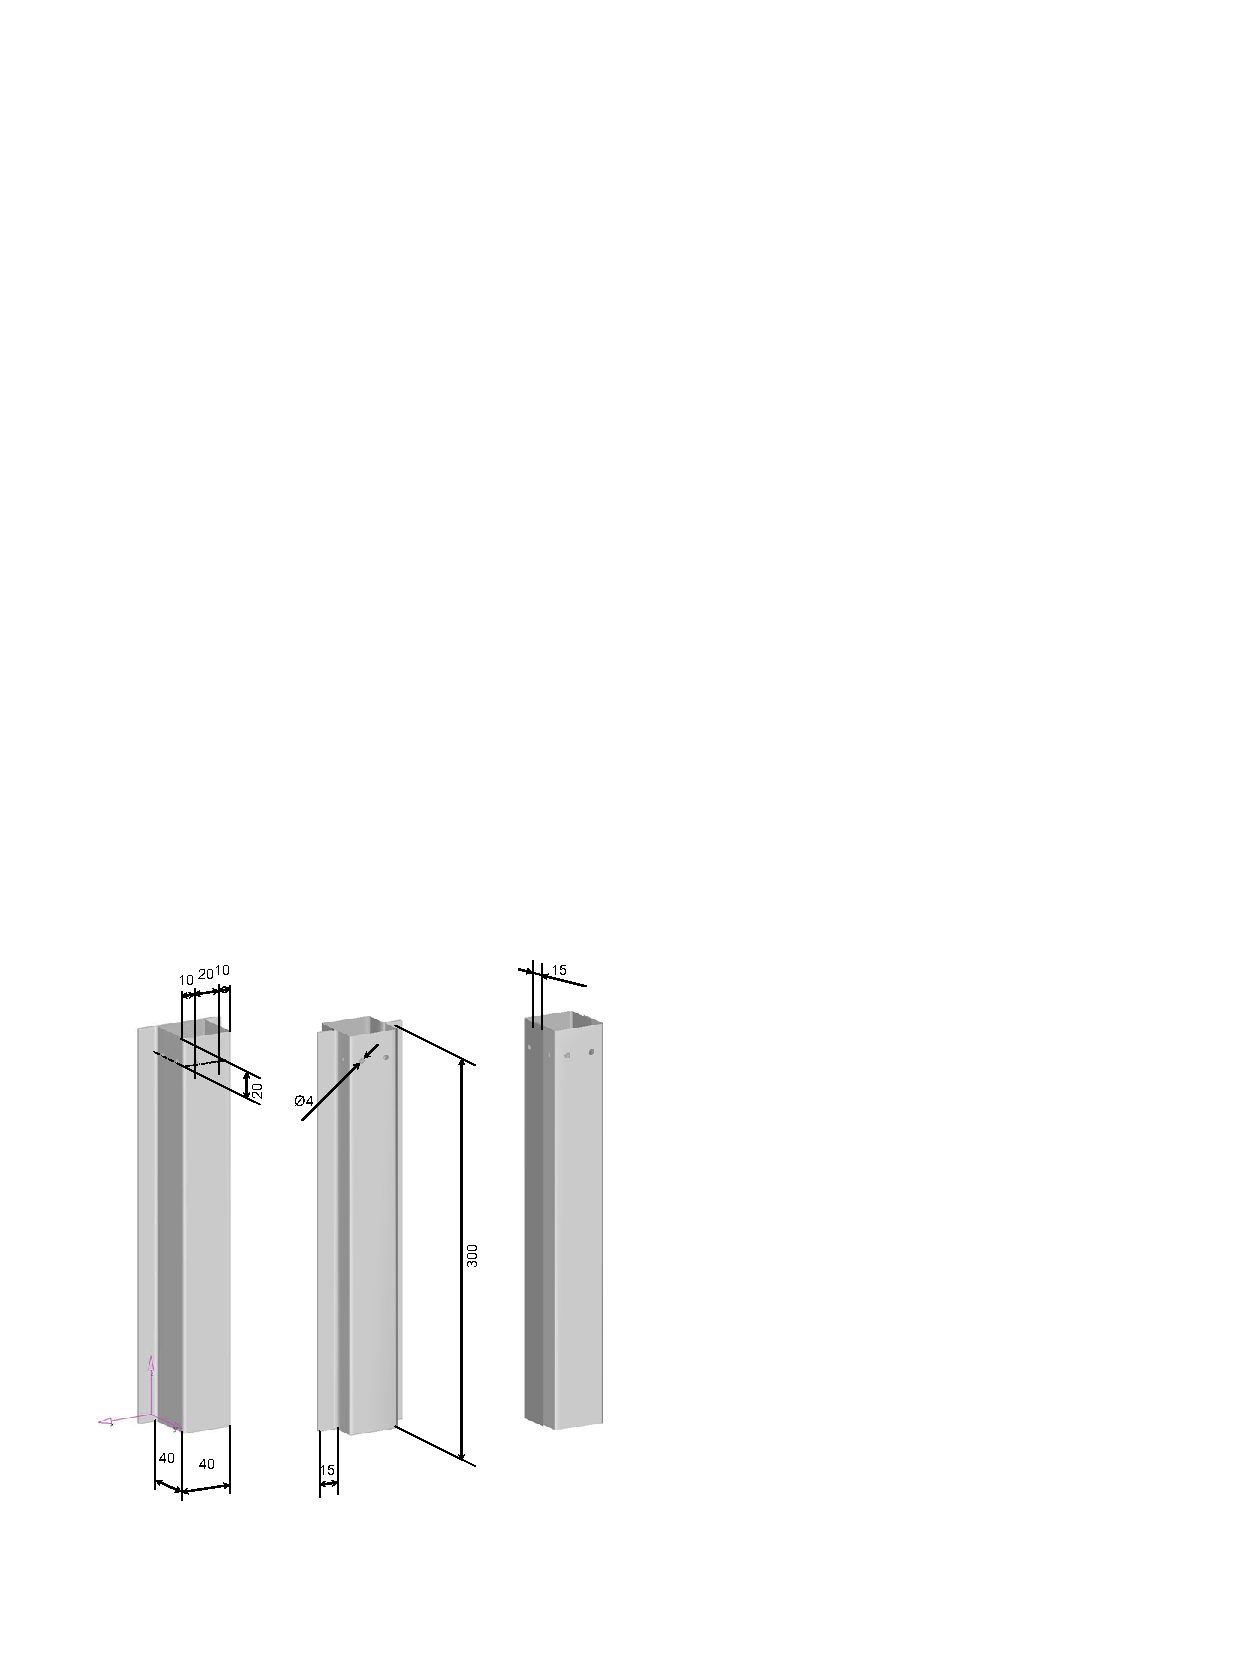
\includegraphics[width=0.6\linewidth]{IMG_CUTRES/crash_box}
	\caption[General measure of the crash box model with three different sections.]{General measure of the crash box model with three different sections. Taken from \citet{Peroni2009}.}
	\label{fig:crash_box}
\end{figure}

\subsection{Triggering}

In order to facilitate the generation of an stable collapse mechanism, crash boxes usually have some triggering in certain areas. It is based on certain controlled weakening of a section of the tube so, when crushing starts, the collapse will tend to a known pattern instead of others. This is done because this stable collapse patterns give the greatest \acrlong{SEA} with reduced \acrlong{Pk}.

In the present study, the trigger system consists on a series of holes placed at $\SI{20}{\mm}$ measured from the crushing end, with a diameter of $\SI{4}{\mm}$, as detailed on \cref{fig:crash_box}. They are meant to weaken the section in which they are applied in order to initiate collapse in that point. Collapse should start as a first wave in that cross section if triggering has been correctly applied.

\begin{figure}
	\centering
	\begin{minipage}[b]{.23\linewidth}
		\centering
		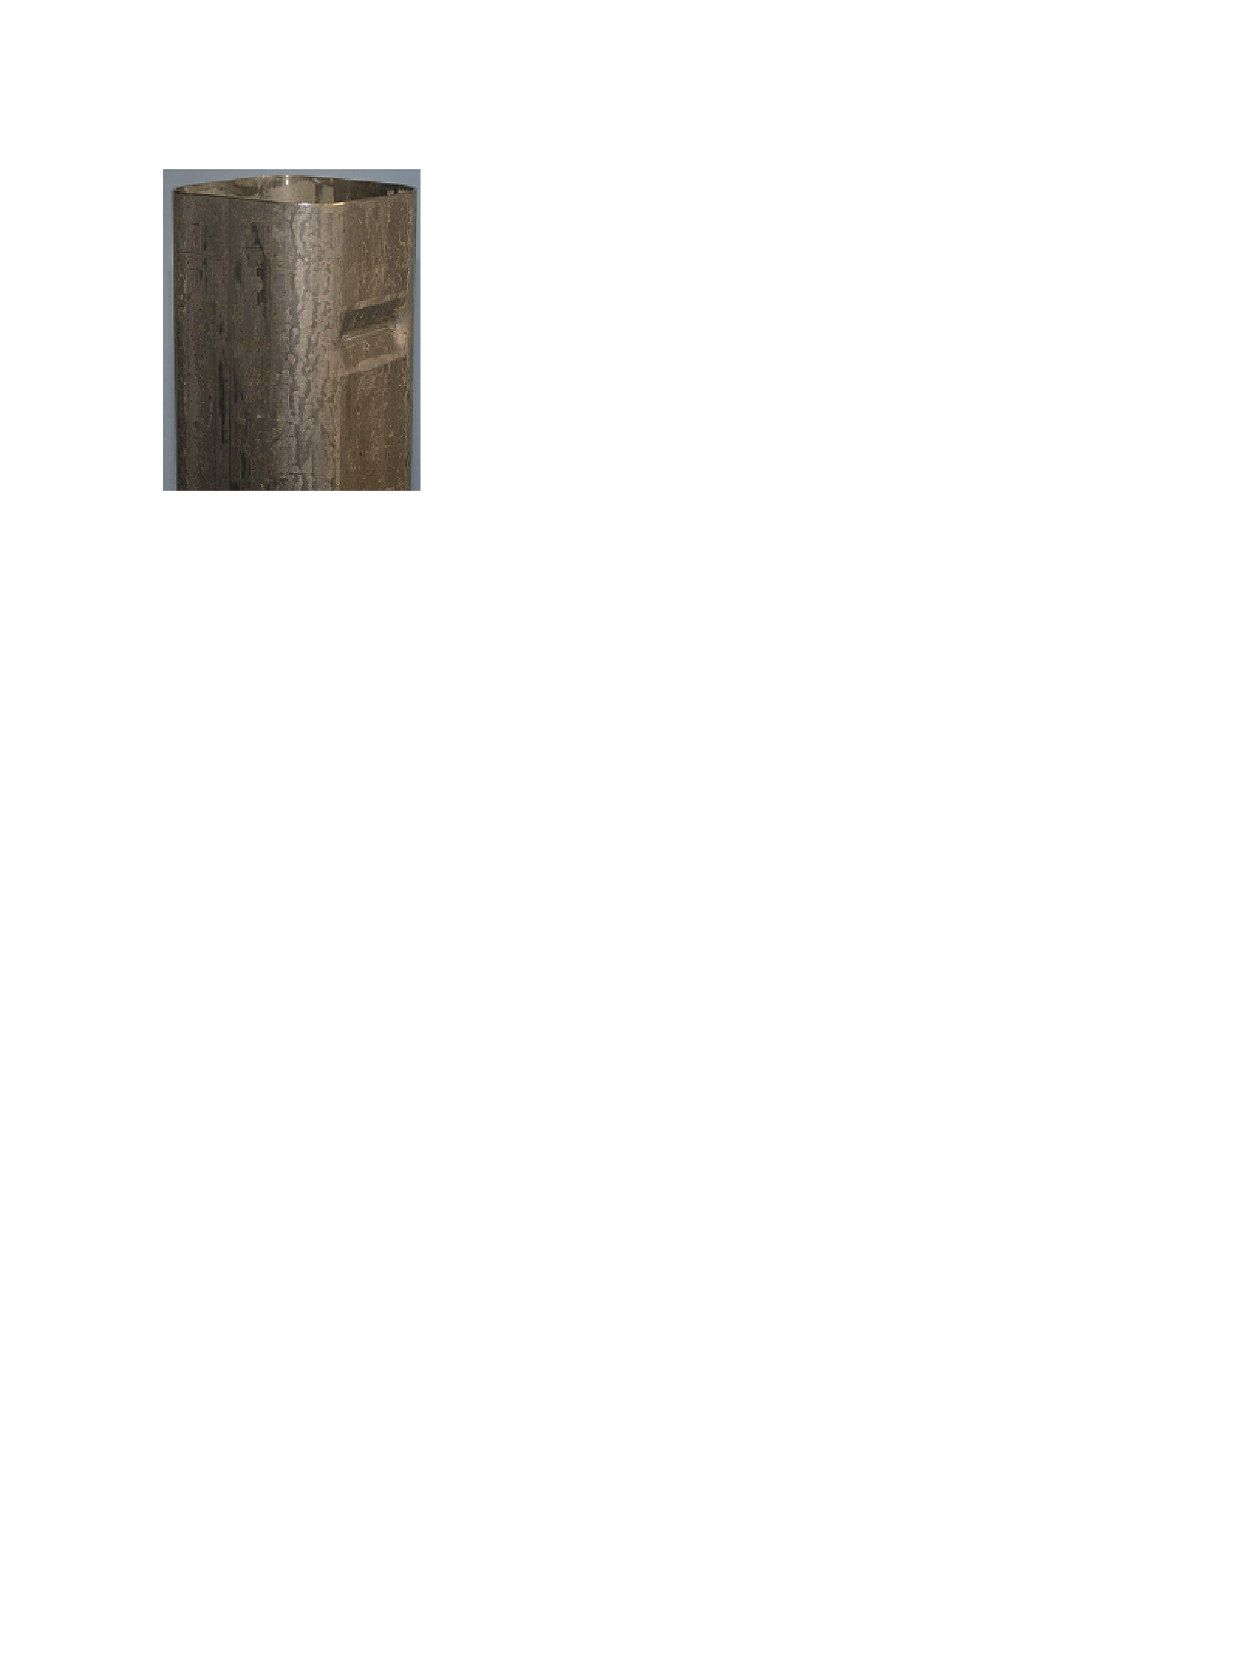
\includegraphics[width=\linewidth]{IMG_CUTRES/abedrabbo_trigger}
	\end{minipage}
	\quad
	\begin{minipage}[b]{.23\linewidth}
		\centering
		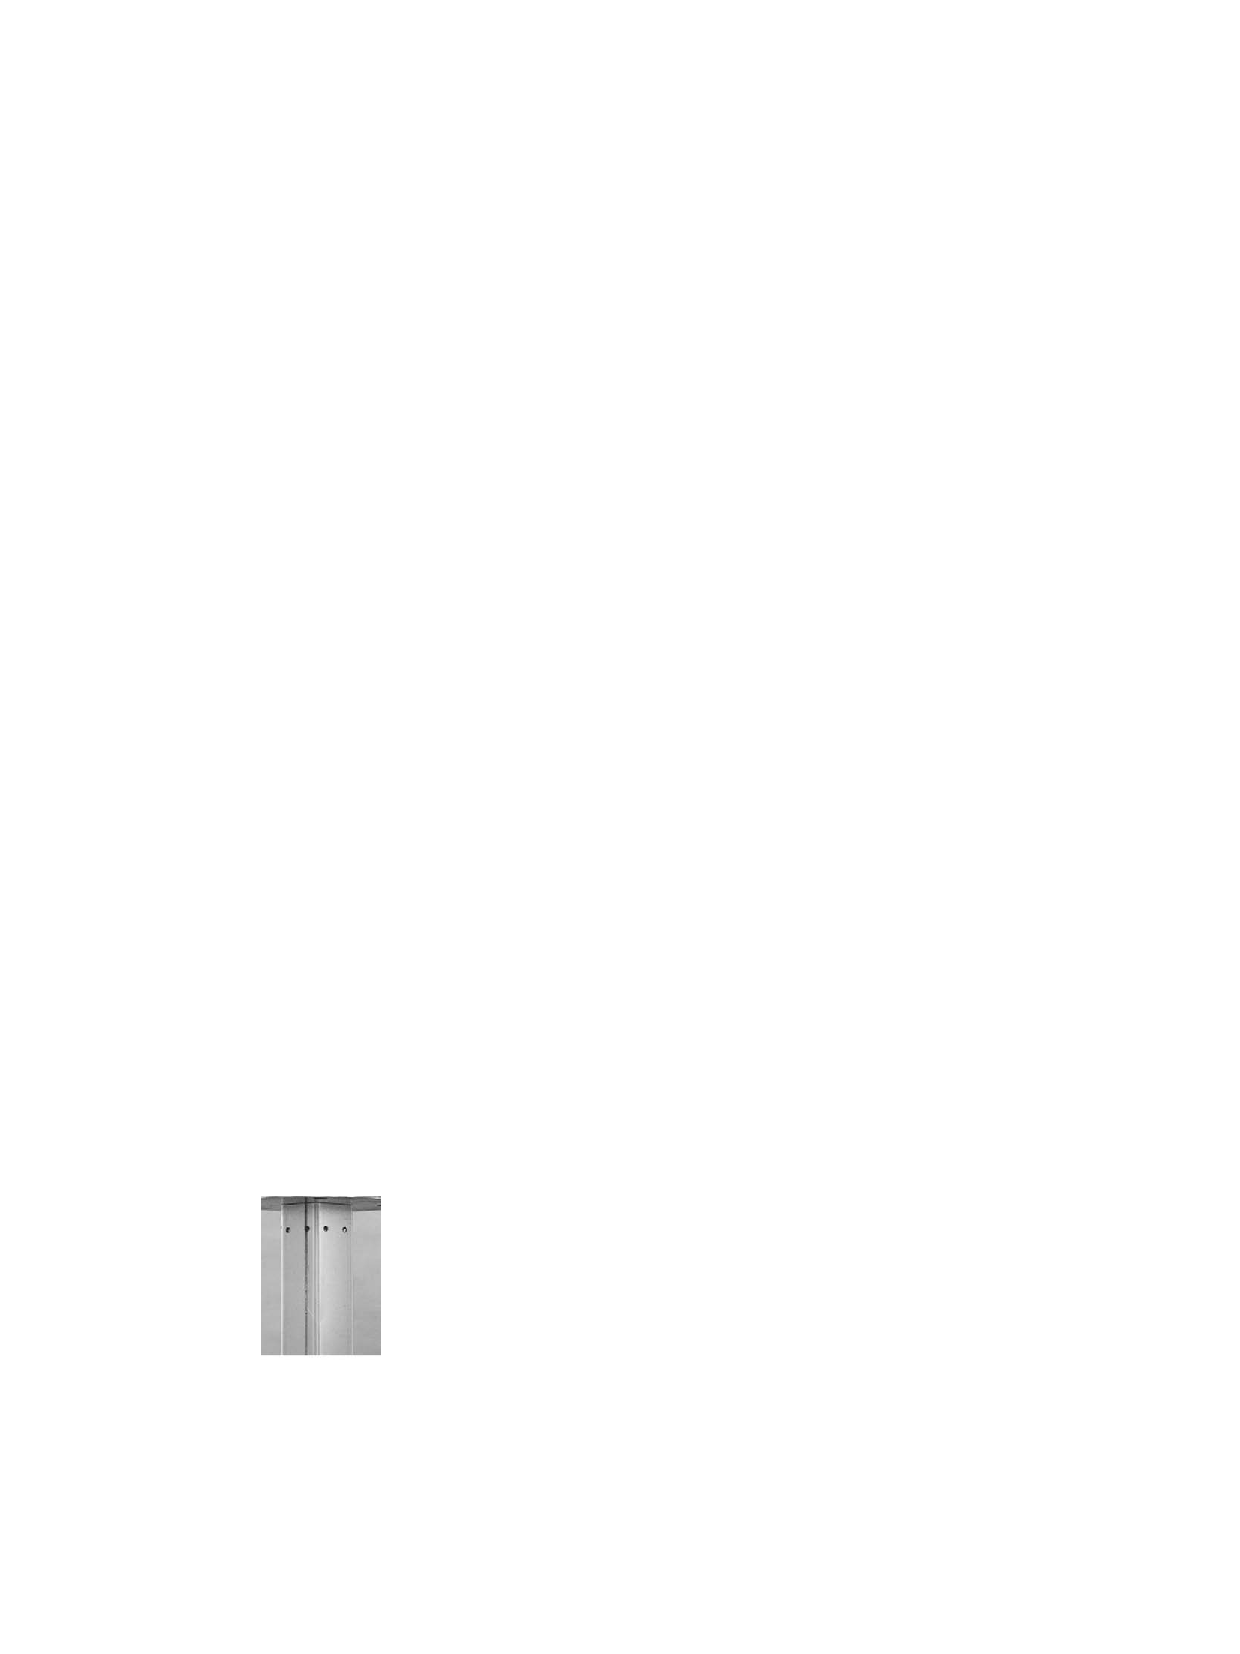
\includegraphics[width=\linewidth]{IMG_CUTRES/peroni_trig}
	\end{minipage}
	\quad
	\begin{minipage}[b]{.45\linewidth}
		\centering
		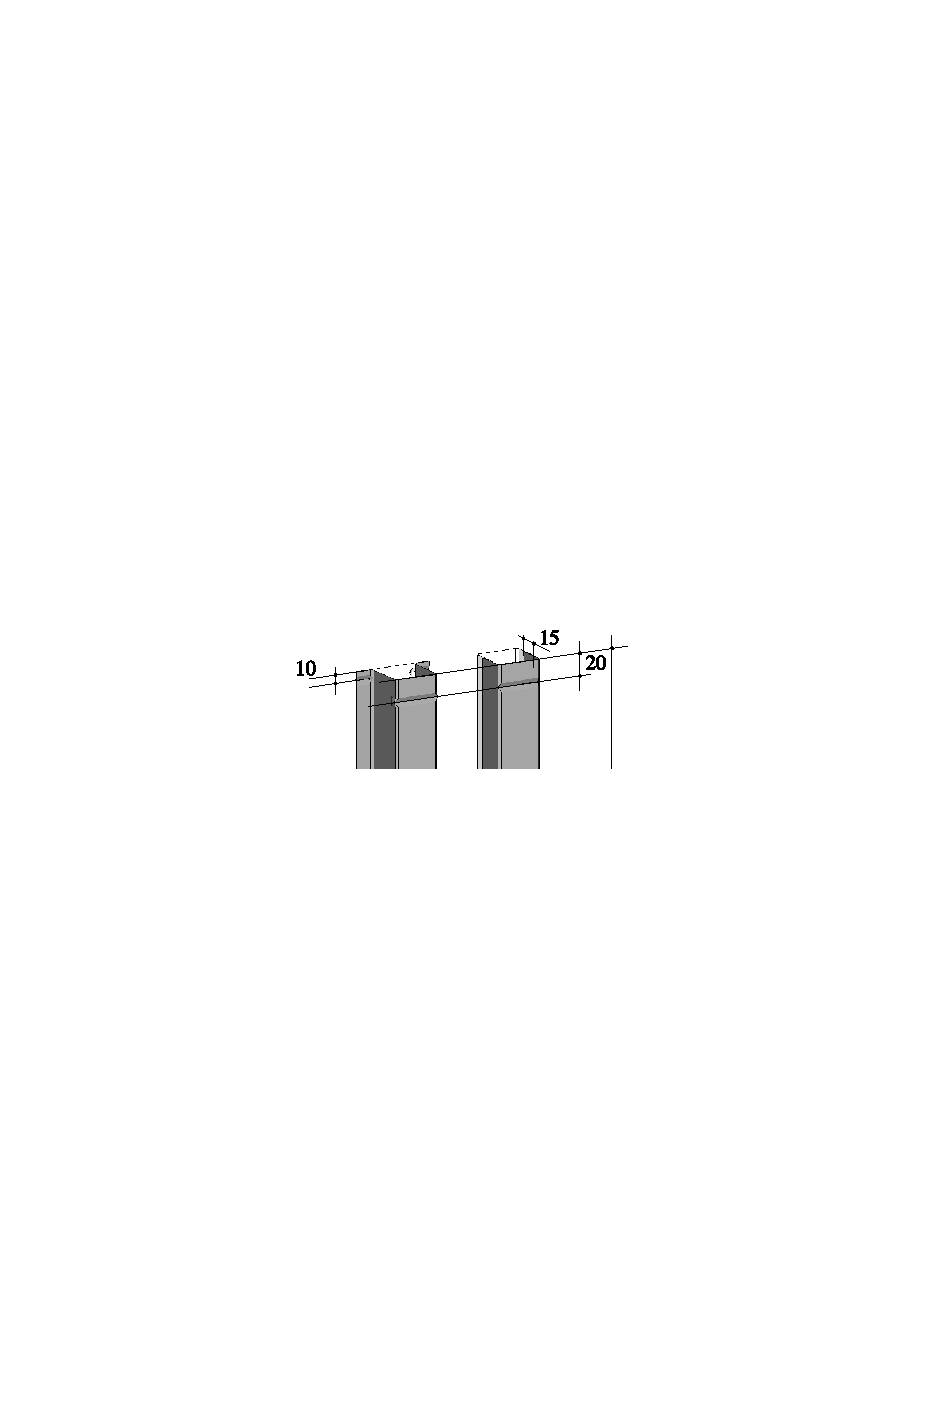
\includegraphics[width=\linewidth]{IMG_CUTRES/scattina_trig}
	\end{minipage}
	\caption[Detail of different triggers: punching, holes and indentations.]{Detail of different triggers. From left to right: punching \citep{Abedrabbo2009}, holes \citep{Peroni2009} and indentations \citep{Scattina2011}.}
	\label{fig:different_trig}
\end{figure}

% Comment other triggers
This is not the only trigger design, as it can be seen on \cref{fig:different_trig}. Initial deformation of a near-head cross section is a common solution \citep{Abedrabbo2009, Scattina2011, Costas2013}, although it may present some problems, such as beginnings of peeling near the triggered section, either provoked by the trigger process itself or either due to easing this peeling in the first phases of the impact.

\subsection{Impact conditions}  % Speed, etc
\label{sec:impact}

The tube was placed between two circular rigid plates, as it can be seen on \cref{fig:general}, one next to the impact head and the rear one next to the opposite end. The impact plate had a initial separation of $\SI{1}{\mm}$ to avoid simulation problems.

\begin{figure}
	\centering
	\begin{minipage}[b]{.22\linewidth}
		\centering
		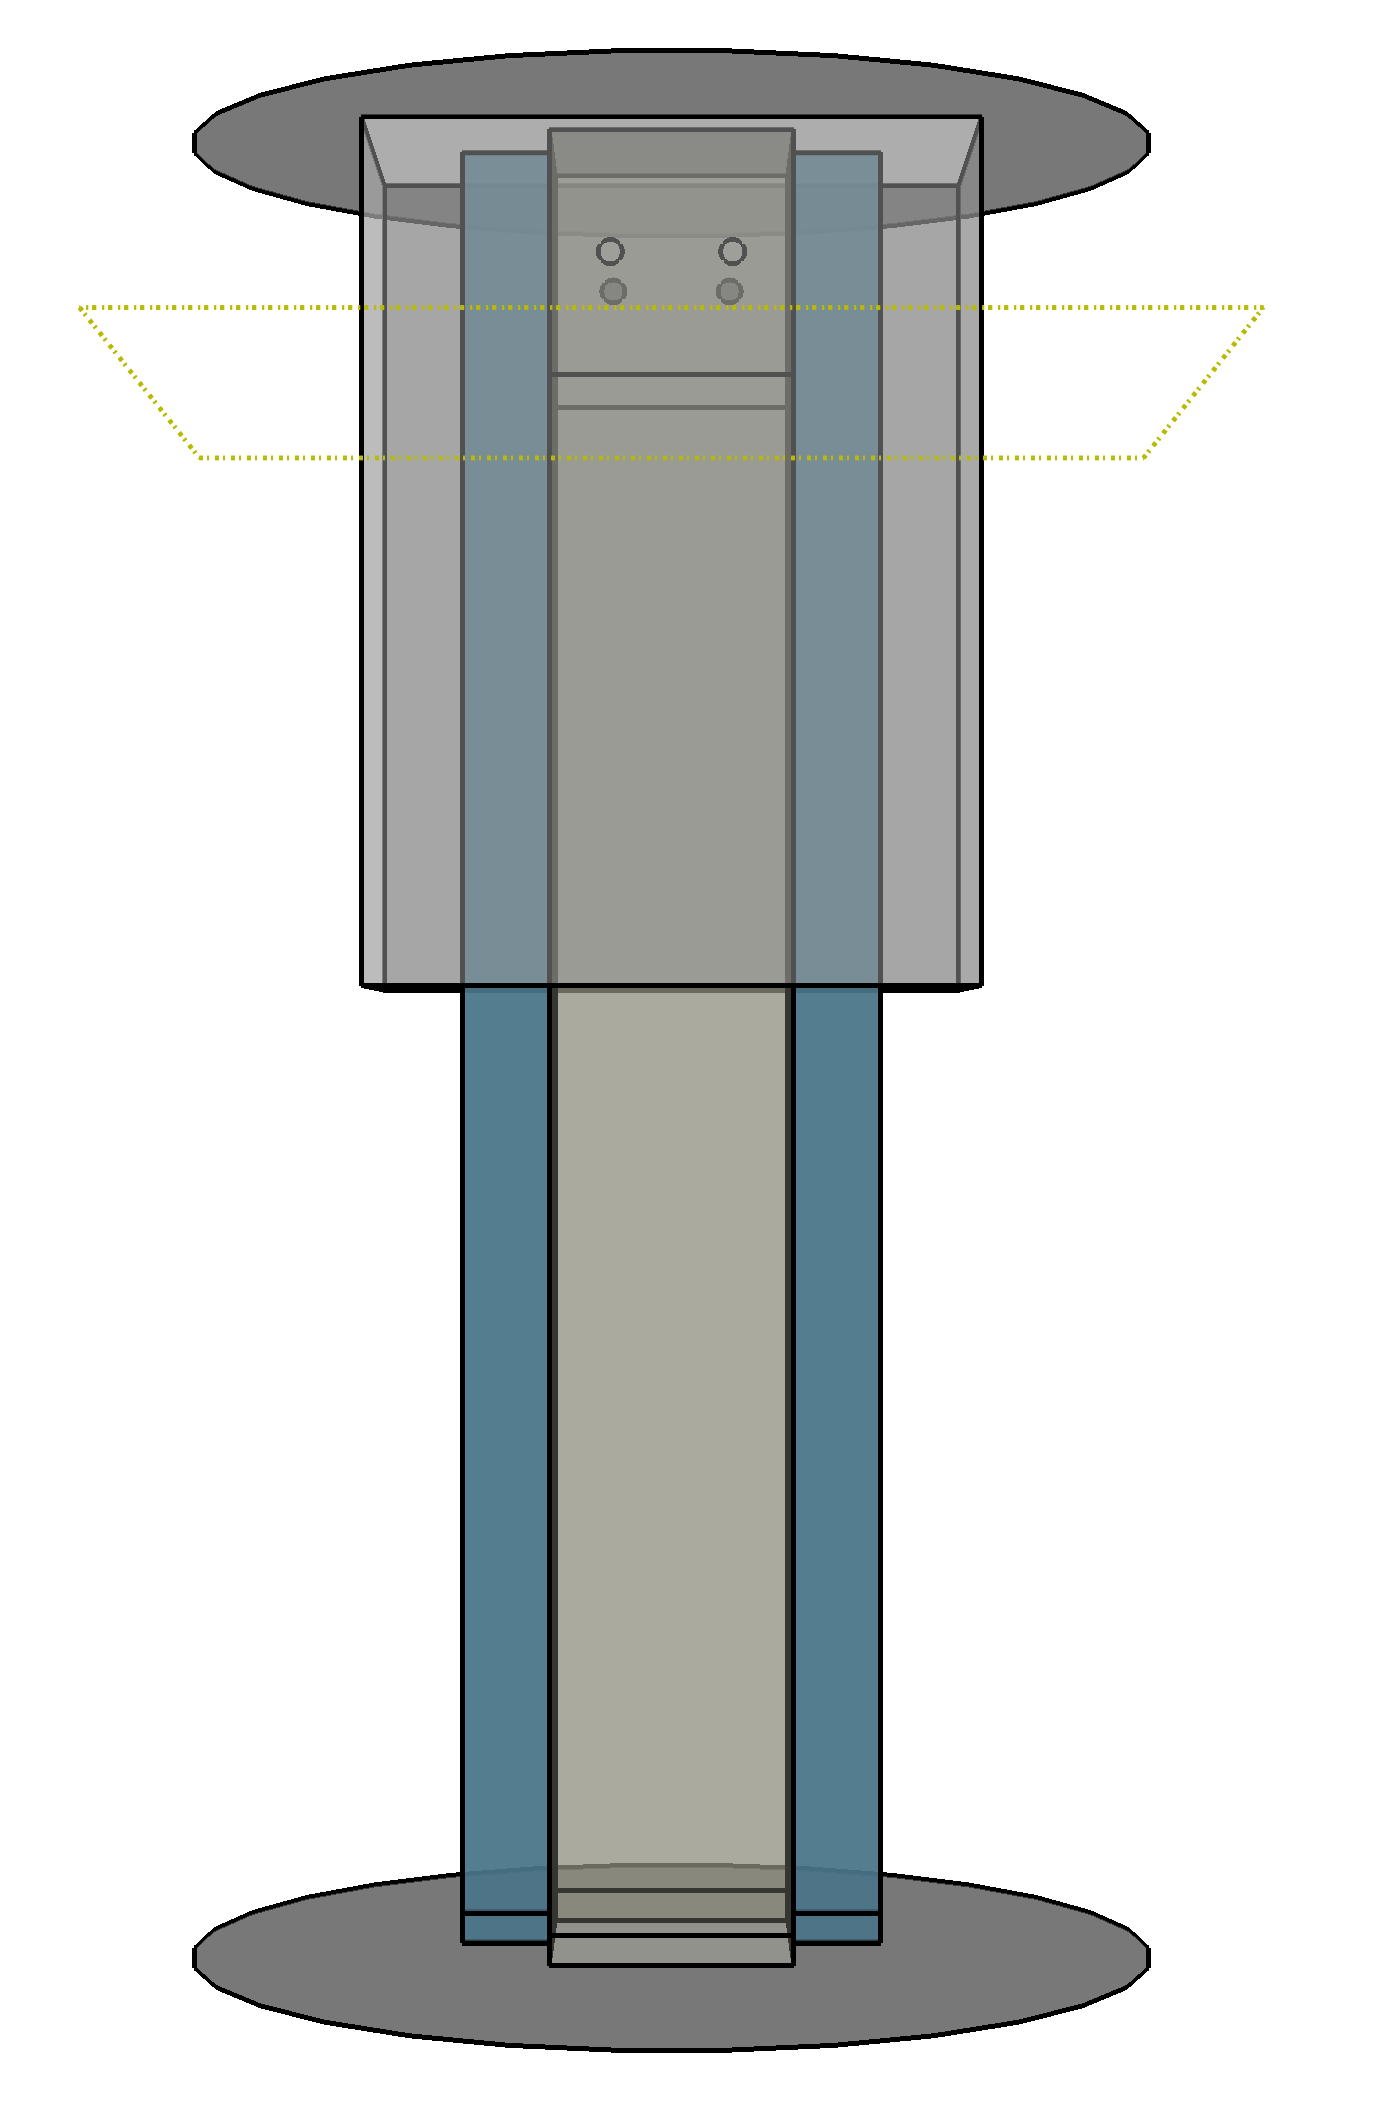
\includegraphics[height=5cm]{IMG_CUTRES/general_transp}
	\end{minipage}
	\quad
	\begin{minipage}[b]{.22\linewidth}
		\centering
		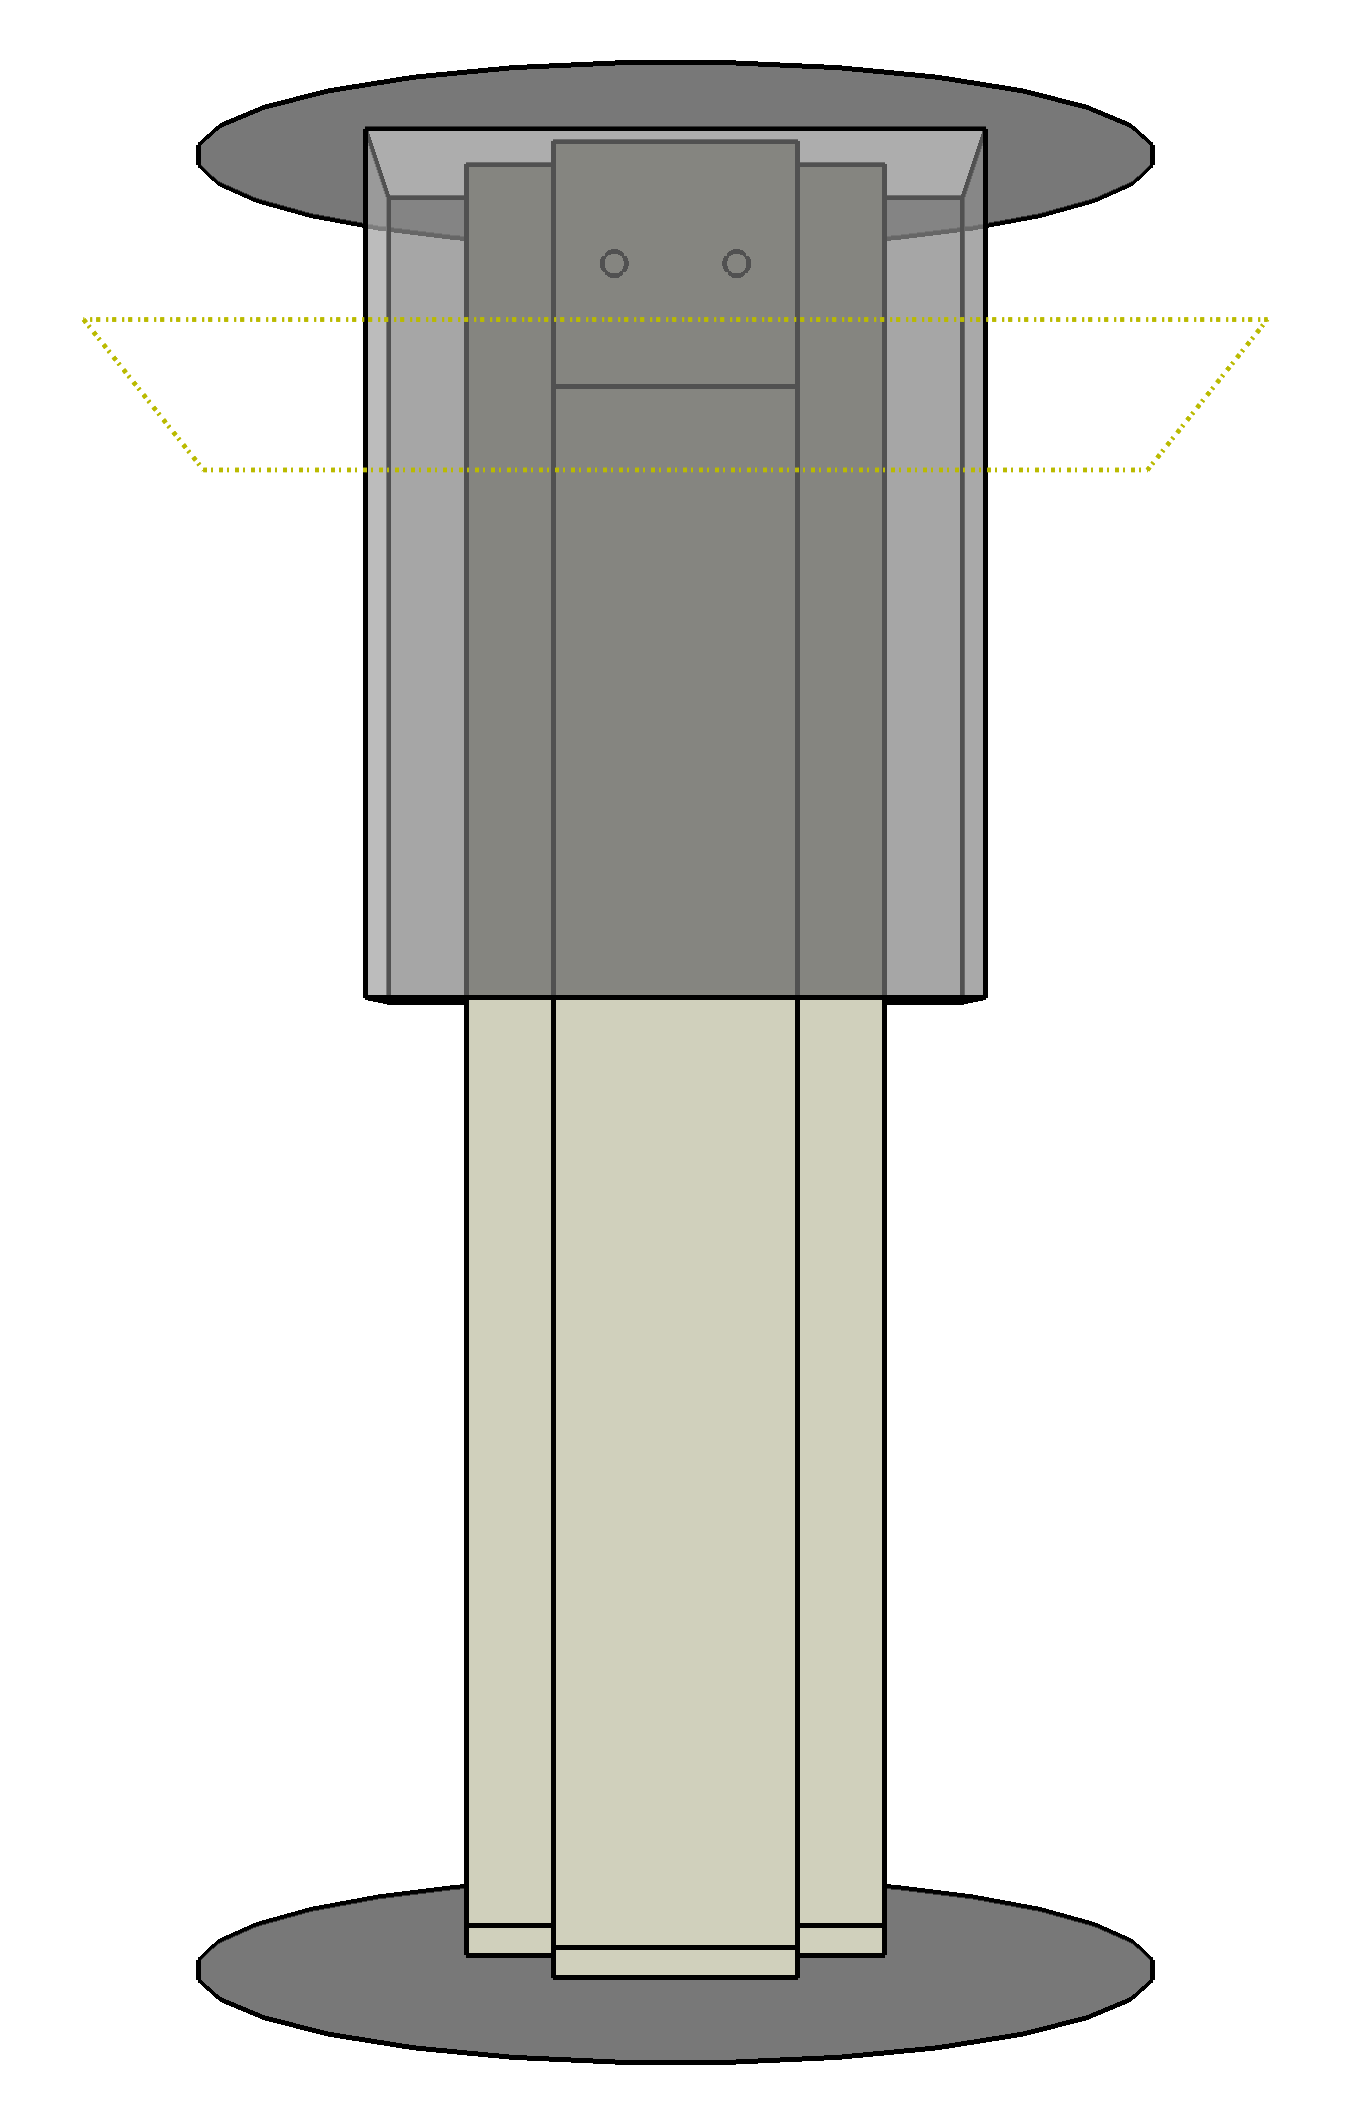
\includegraphics[height=5cm]{IMG_CUTRES/general_rigtransp}
	\end{minipage}
	\quad
	\begin{minipage}[b]{.22\linewidth}
		\centering
		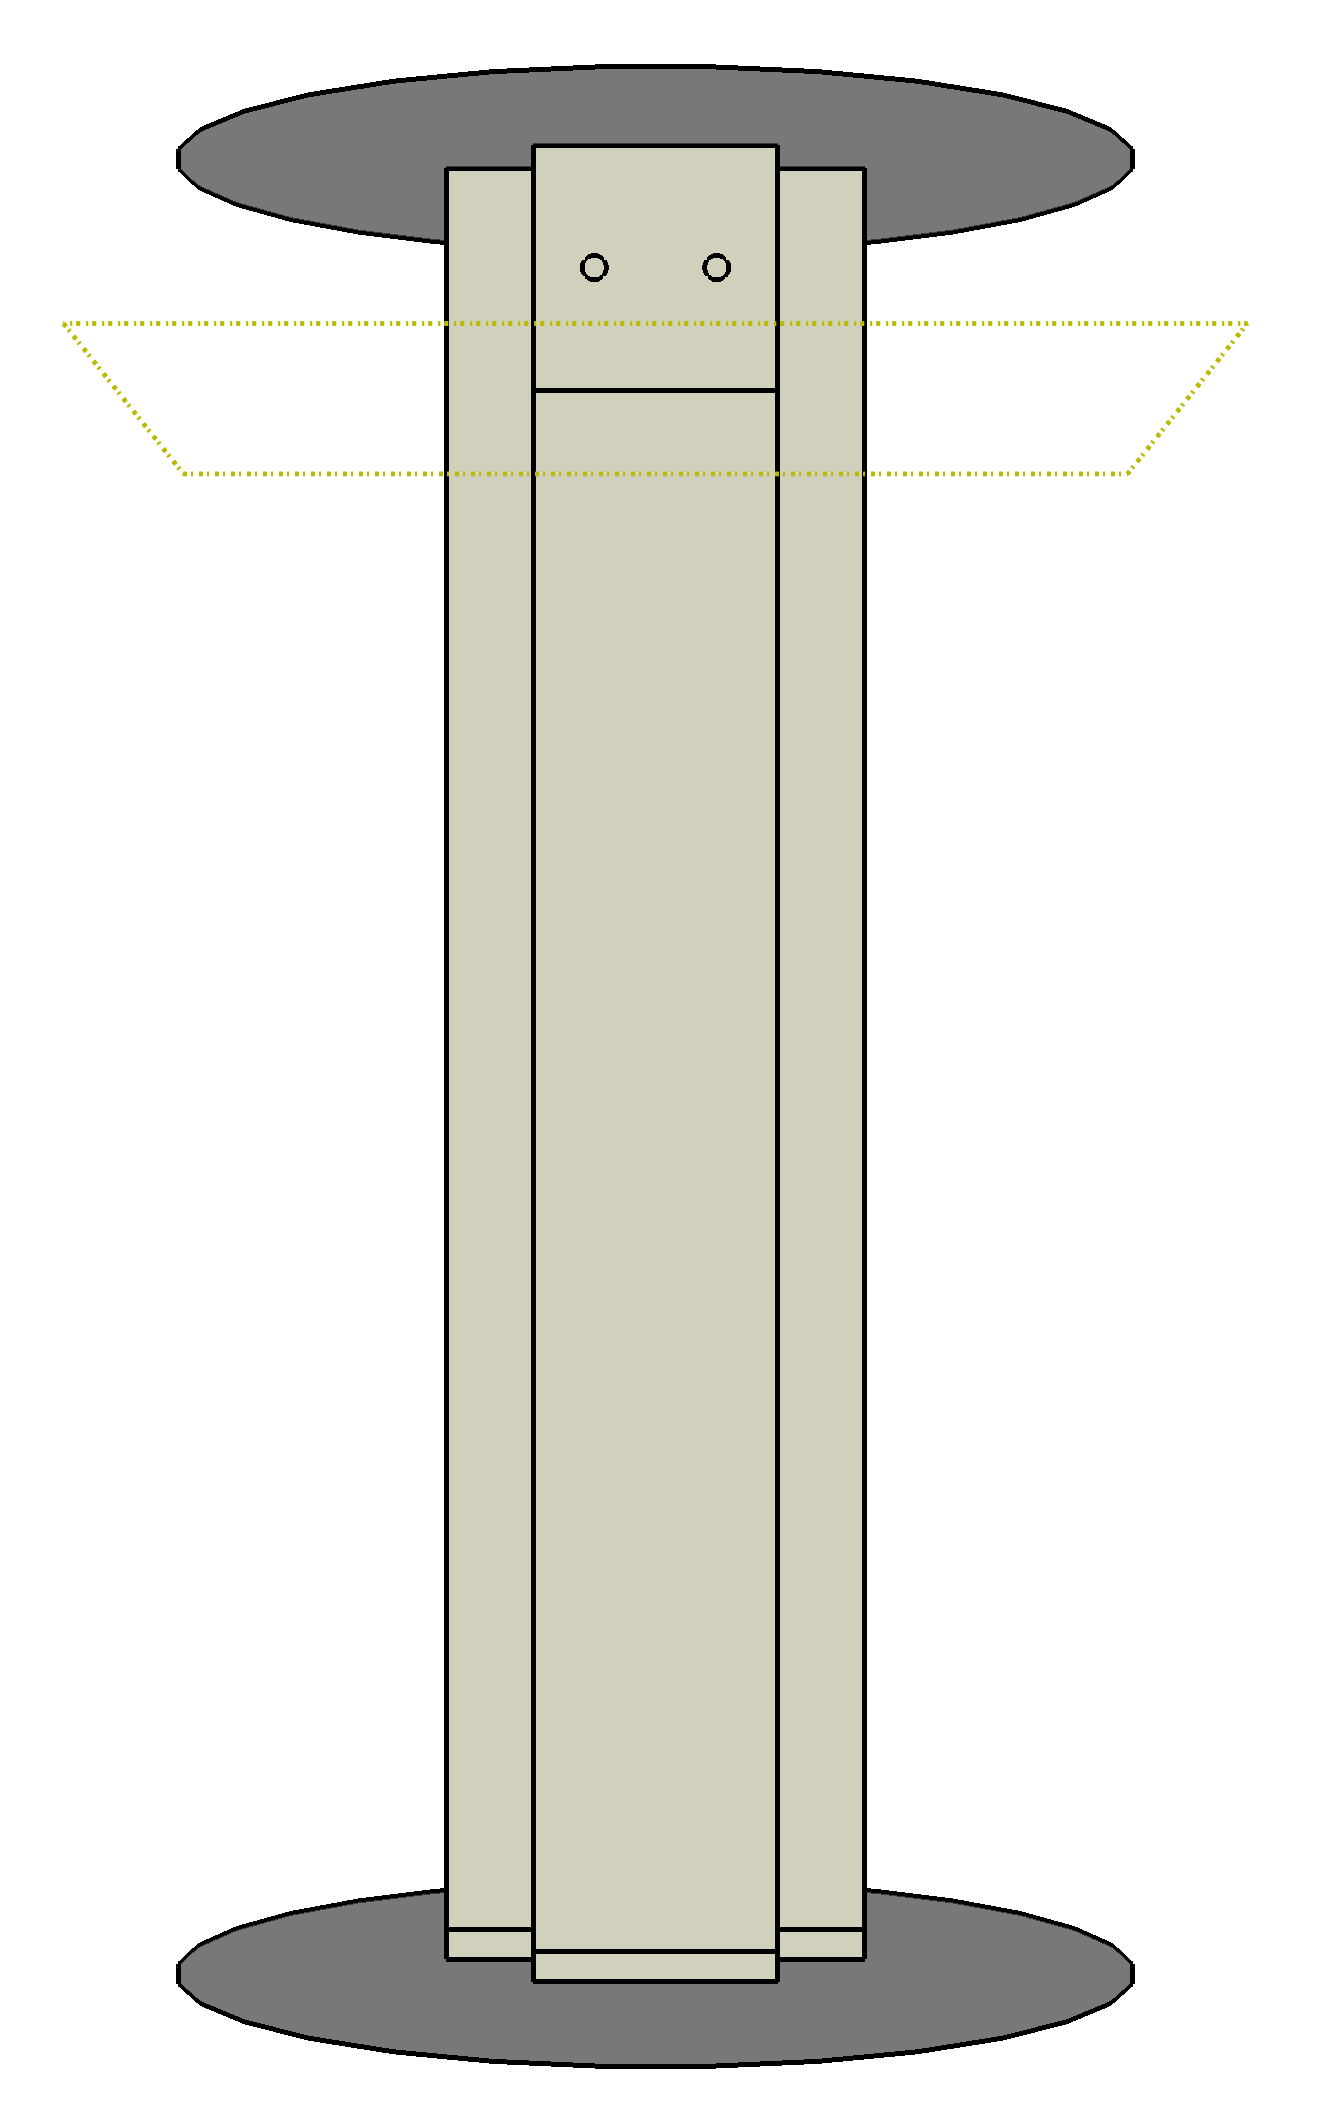
\includegraphics[height=5cm]{IMG_CUTRES/general_noSb}
	\end{minipage}
	\quad
	\begin{minipage}[b]{.22\linewidth}
		\centering
		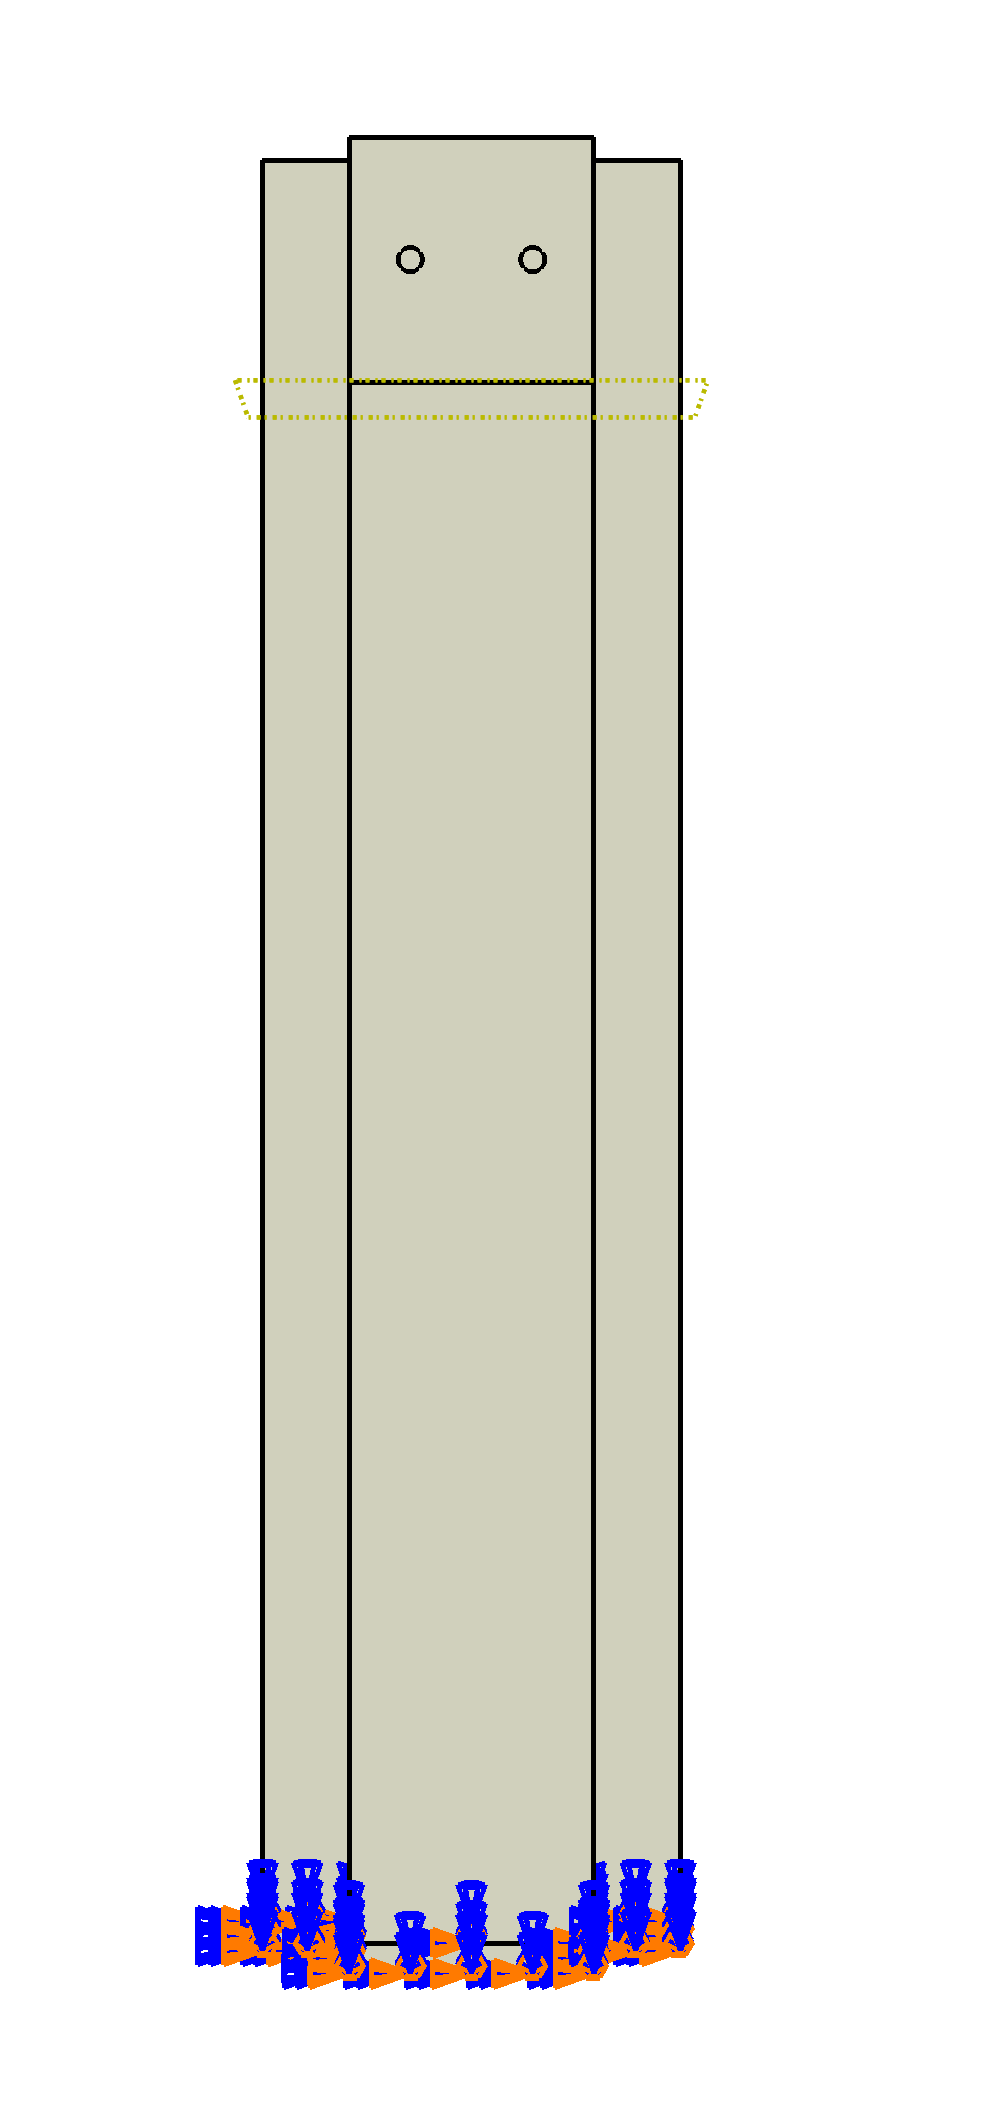
\includegraphics[height=5cm]{IMG_CUTRES/general_encastre}
	\end{minipage}
	\caption[General view of the model.]{General view of the model. Crushing from up to down. From left to right: view with transparency (adhesive in blue); view with rigid parts transparency; view without stabilizing box; view with the fixed part highlighted.}
	\label{fig:general}
\end{figure}

In the bibliography, impact tests are often substituted by quasi-static tests, due to the similarities between both with materials with low sensitivity to strain ratio. References including actual impact tests usually compare both situations \citep{Goglio2008, Peroni2009}, concluding that these two ways of facing this problem are not always equivalent. In this study, a full impact simulation was carried out. The objective is to develop systems that behave in the same manner both in static or low velocity tests and on impact  tests.

The impact plate moved during the simulation at $\SI{10}{\m/\s}$ on a total distance equal to half of the total tube's length, resulting in a total analysis time of $\SI{0.015}{\s}$ long. Rotational degrees of freedom were fixed on the frontal plate.

The rear plate had all degrees of freedom restrained. The reaction force that appeared on this point was used to measure \gls{Ea}, as explained later on (see \cref{sec:Ea}).

The last $\SI{5}{\mm}$ of the crash tube had all degrees of freedom fixed (see \cref{fig:general}), except displacement on the impact direction in order to allow the reaction force measurement commented before. This way, numerical issues due to excesive unrestrained degrees of freedom on the whole tube were prevented.

\subsubsection{Rivets}

Peeling problems were found near the impact head end during the development of the study. \citet{Peroni2009} solved this situation by adding two rivets on the bonded flanges at the triggered section in order to avoid excesive debonding on that part of the tube in the initial phases of the impact and, thus, prevent critical situations. In this study, it was substituted by a $\SI{2}{\mm}$-diameter spot-weld point in the same location, as it was a better-known technique for the author and had a very similar effect on the model.

% INSERT IMAGE TO EXPLAIN LOCATION

The spot weld was made up of steel, using its elastic modulus as stiffness and the steel plastification stress on the normal direction as the failure criterion. Several sizes for the spot-weld points were tried up to an average solution which wasn't either too strong to obviate the adhesive's contribution, neither too weak to not prevent the critical failure.

\subsubsection{Stabilizing box}

Due to the crushing conditions and the relation between tube length and cross section area, strong difficulties were found in order to achieve stable collapse mechanisms. On their place, tubes diverted from their axis ---other found problems not related with the tube bending are solved through the use of rivets---. Trying to avoid these critical situations, four rigid plates on a rectangular section among the crash tube were added to the model as a stabilizing box.

It has half of the length of the tube and moved together with the impact plate, so the crash tube would end confined between the plates on both ends and the stabilizing box by the end of the simulation. Its section was of $\num{100}\times\SI{60}{\mm}$ and co-centered with the crash box.

The rationale behind this is that in an actual vehicle crash, this device would be among many other vehicle parts ---such as the motor, which is very rigid---, restraining the crash box movements in many directions. It also aims to prevent global buckling problems.

\section{Materials}

The model is made up of two different materials, together with several already mentioned ideally rigid parts (see \cref{sec:impact}). The adherends of the tube are made of elastic-plastic steel. The adhesive is an elastic material only considering one normal and two shear directions with a damage formulation.

It must be pointed out that the use of several material with different behaviour formulations including crack formation implies the use of the \gls{XFEM}. Although it will have some implications in the present section ---and more specifically on \cref{sec:damage}---, the \gls{XFEM} will be explained afterwards in \cref{sec:xfem} in order to keep some coherence in the explanation.

\subsection{Adhesive}
Loctite Hysol 9514 \citep{manufCatalog} was the chosen adhesive for the bonding, for its shown interest by many other authors for structural bonding \citep{Sadowski2010, Scattina2011, SernaMoreno2015}, making it an \textit{a priori} good candidate for the studied application. It is a monocomponent epoxy adhesive which requires heat curing processes in the union cast.

According to \citet{manufCatalog}, the shear strength of the adhesive is $\SI{44}{\MPa}$, although this parameter is subject to variation depending both in cure temperature and time. Dependency can be seen on \cref{fig:catalog_temp}. Given value corresponds to a $\SI{150}{\celsius}$ cure for $\SI{30}{\min}$. The bulk modulus is $\SI{1460}{\MPa}$ and the adhesive's density is $\SI{1.46}{\tonne/\m^3}$ \citep{manufCatalog}.

\begin{figure}
	\centering
	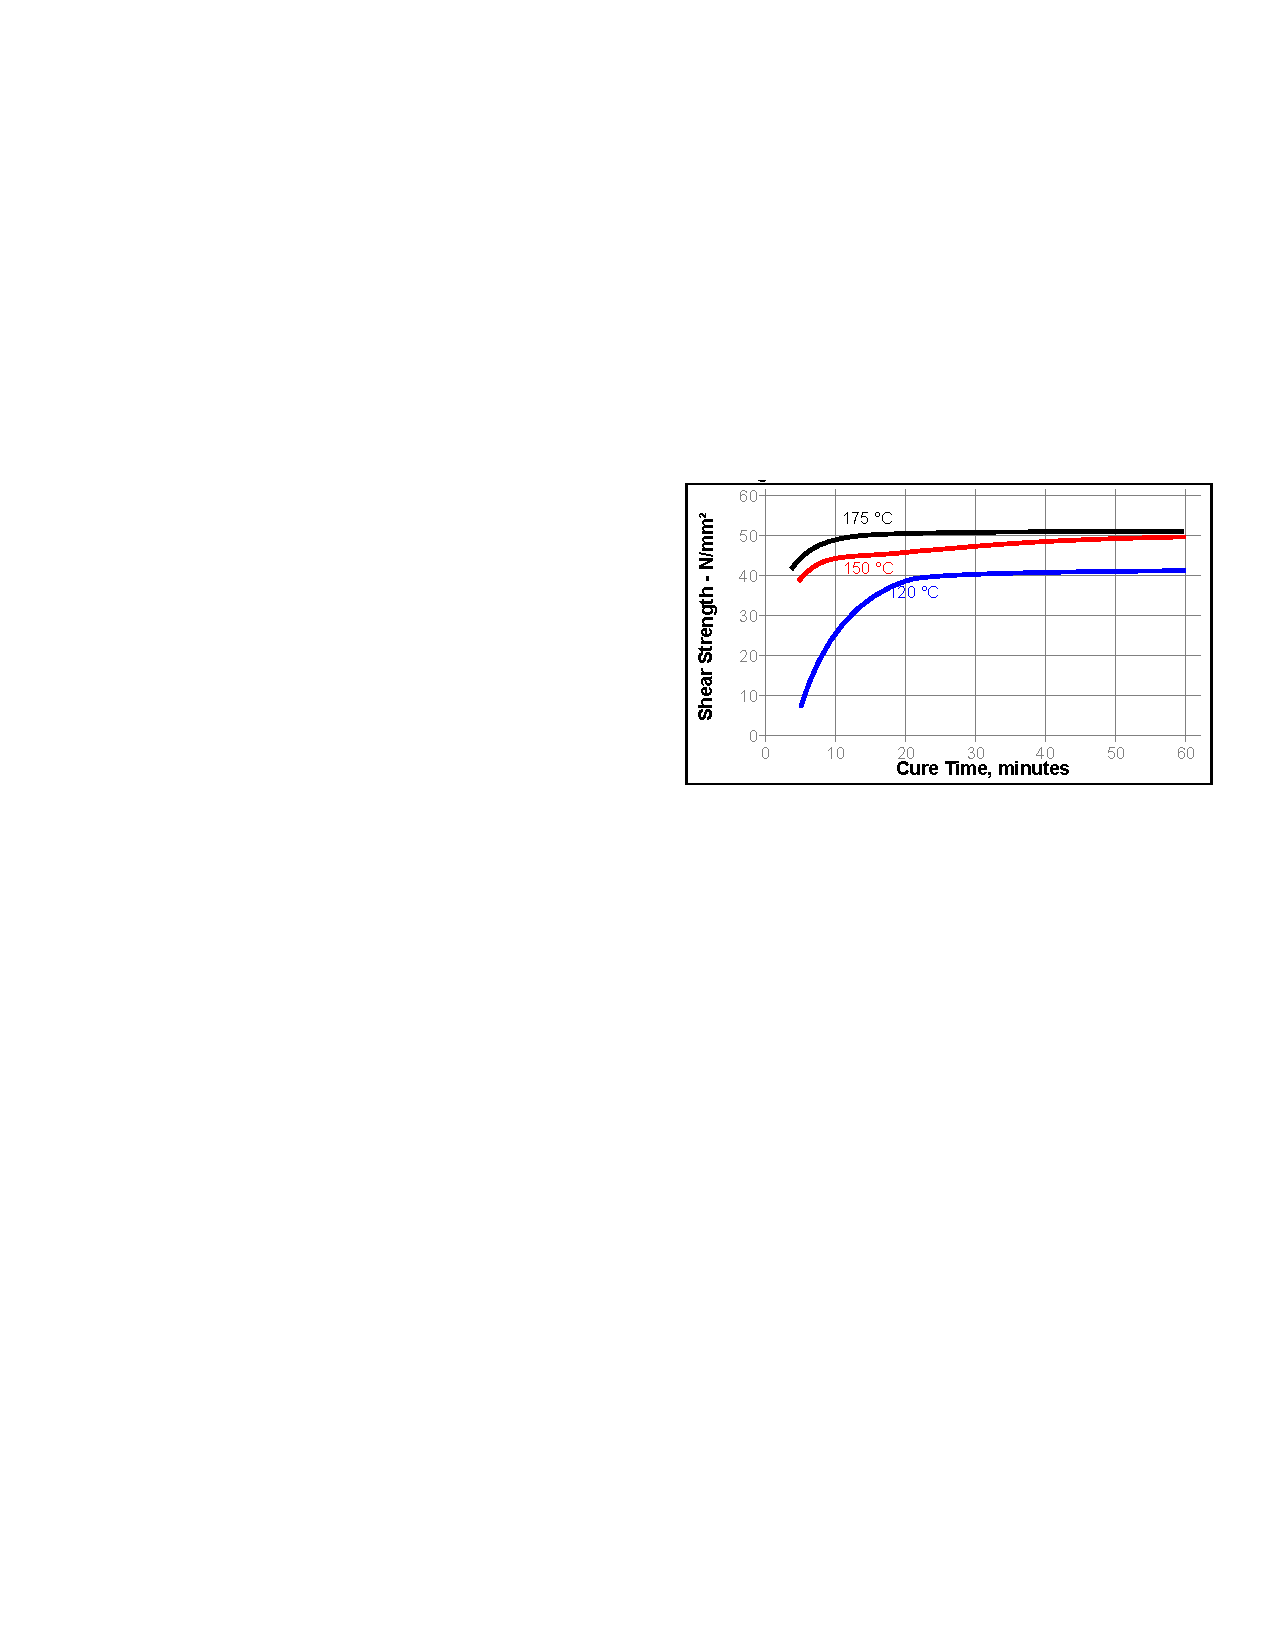
\includegraphics[width=0.7\linewidth]{IMG_CUTRES/catalog_temp}
	\caption[Cure temperature and time dependency of the Loctite Hysol 9514 shear strength.]{Cure temperature and time dependency of the Loctite Hysol 9514 shear strength. Taken from \citet{manufCatalog}.}
	\label{fig:catalog_temp}
\end{figure}

\subsubsection{Constitutive behaviour}
\label{sec:elastic}

The constitutive behaviour was supposed to be isotropic linear elastic \citep{SernaMoreno2015} up to failure start. An uncoupled traction elastic behaviour \citep{Sadowski2010, Sadowski2011, Scattina2011, Sadowski2014} on 3D cohesive finite elements was the best fit for modelling adhesives \citep{Abaqus613Manual}. \Cref{sec:coh_elem} deepens on the element formulation and properties. \Cref{eq:traction} shows how this model works.

\begin{equation}
\begin{Bmatrix}
t_n \\
t_s \\
t_t \\
\end{Bmatrix}
=
\begin{bmatrix}
E_{nn} & & \\
& E_{ss} & \\
& & E_{tt} \\
\end{bmatrix}
\begin{Bmatrix}
\varepsilon_n \\
\varepsilon_s \\
\varepsilon_t \\
\end{Bmatrix} ;
\label{eq:traction}
\end{equation}
where $t_n$ is the nominal traction in the normal direction; $t_s$ and $t_t$ are the nominal tractions in both shear directions; $E_{nn}$, $E_{ss}$ and $E_{tt}$ are the corresponding stiffnesses; and $\varepsilon_n$, $\varepsilon_s$ and $\varepsilon_t$ are the corresponding nominal strains \citep{Abaqus613Manual}. $E_{ss}$ is considered equal to $E_{tt}$, and this value will be refered as $E_{T}$ onwards. In order to match this nomenclature, $E_{nn}$ will be refered as $E_{N}$.

It is remarked that \cref{eq:traction} relates forces and strains ---not forces and displacements, or stresses and strains, as usual---, implying thus that the value of $E_{N}$ depends on the thickness of the layer. As \cref{eq:traction} refers to each element, the value of $E_{N}$ depends not only on the mentioned geometry, but also on the mesh. In this case, it can be calculated by dividing the elastic modulus, $E$, by the adhesive layer thickness.

This may bring up some problems in those cases in which the adhesive layer has a non-uniform thickness, or very different element lengths between different zones of the material. In our case, elements have fairly uniform in-plane sizes, and the layer has a uniform thickness for the normal direction.

The constitutive model expresed in \cref{eq:traction} is an orthotropic model that only applies in one direction: the stack direction, as refered in \cref{sec:coh_elem}. The reduced adhesive layer thickness makes in-plane compression negligible. Uncoupled behaviour of the elastic components is not considered \citep{Scattina2011}.

\citet{Scattina2011} obtained adhesive stiffnesses through the inverse method, which are summarized in \cref{tab:ads_params}. These same parameters were used in the present study, as their results could be validated with the model.

On the other hand, the elastic modulus in the normal direction can also be calculated using bulk modulus, $K$, provided by \citet{manufCatalog} and a Poisson's modulus, $\nu$, of $\num{0.295}$ \citep{JDiaz}, through the common formula that relates these parameters with the elastic modulus, $E$ in linear elastic mechanics. A similar proceeding would apply for both in-plane shear directions related to the shear modulus, $G$. The values obtained this way would be: $\SI{5.986e9}{\kN/\m^2}$ for $E_{N}$ and $\SI{3.467e8}{\kN/\m^2}$ for $E_{T}$. In spite of that, the values given by \citet{Scattina2011} are finally used.

\begin{table}
	\centering
	\begin{tabular}{llrl}
		\toprule
		Parameter & Description & Value & \\
		\midrule
		$E_{N}$ & Stiffness in normal direction & $\num{5e9}$ & $\si{\kN/\m^2}$ \\
		$E_{T}$ & Stiffness in an in-plane direction & $\num{8e7}$ & $\si{\kN/\m^2}$ \\
		\bottomrule
	\end{tabular}
	\caption[Loctite Hysol 9514 parameters.]{Loctite Hysol 9514 parameters. Taken from \citet{Scattina2011}.}
	\label{tab:ads_params}
\end{table}

\subsubsection{Damage model}
\label{sec:damage}

% Check other authors here
\Cref{fig:Wu_failure_systems} shows the two possible failure mechanisms that may happen in an adhesive union, as described by \citet{Wu2013}:
\begin{itemize}
	\item Adhesive failure, refered to the contact between different materials, implies the separation of the adhesive from the adherend.

	\item Cohesive failure \citep{Vaidya2006}, refered to the bulk material, means that one piece of adhesive gets teared apart from another, breaking the continuum.
\end{itemize}

\begin{figure}
	\centering
	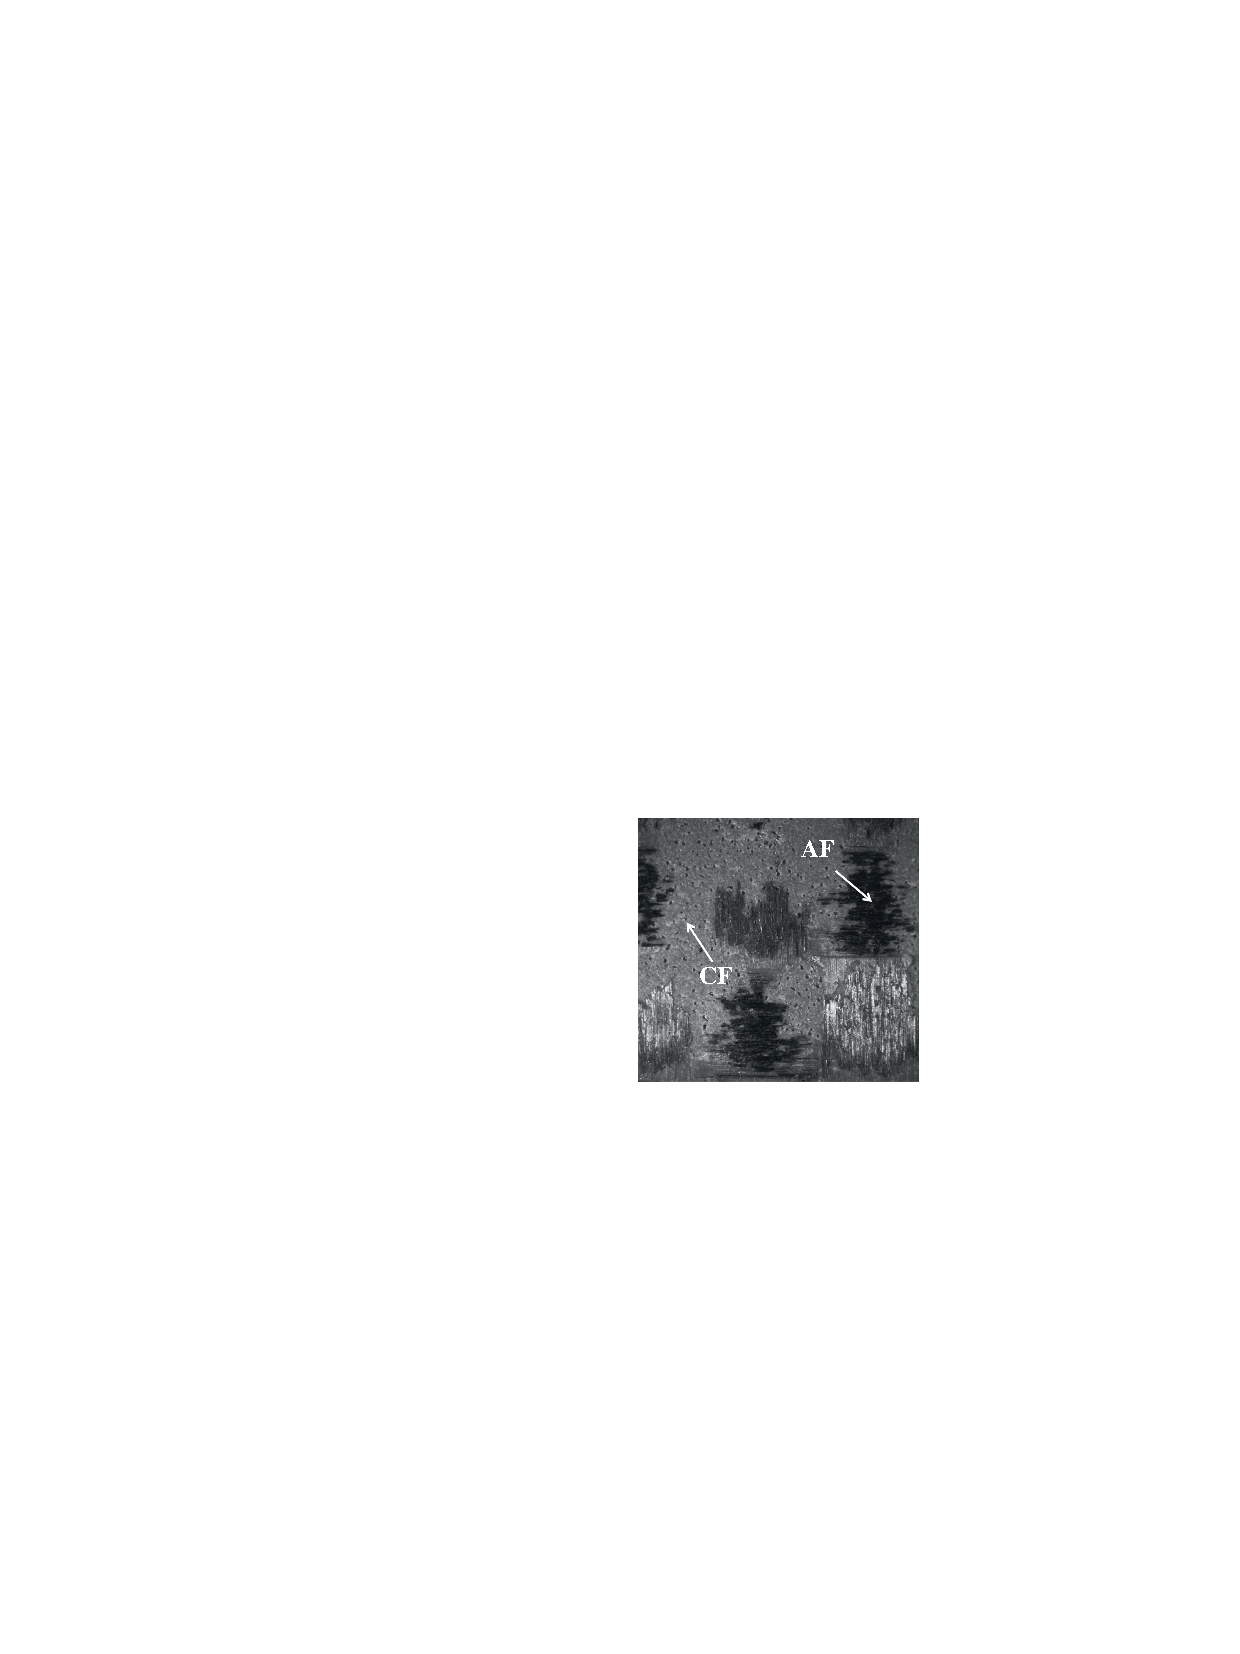
\includegraphics[width=0.7\linewidth]{IMG_CUTRES/Wu_failure_systems}
	\caption[Detail of both possible failure mechanisms of an adhesive union: cohesive failure and adhesive failure.]{Detail of both possible failure mechanisms of an adhesive union: cohesive failure (CF) and adhesive failure (AF). Taken from \citet{Wu2013}.}
	\label{fig:Wu_failure_systems}
\end{figure}

Contact failure modelling ---corresponding to adhesive failure--- resulted in some simulation problems, which are furtherly explained in \cref{sec:coh_elem}. This situation was overcome by including only failure definitions in the bulk material, obviating the contact/adhesive failure as suggested by several authors \citep{Greve2007, Loureiro2010, Sadowski2010, Sadowski2011, Scattina2011, Sadowski2014, SernaMoreno2015}, although the modelled cohesive damage parameters include the effect of both adhesive and cohesive resistance.

The quadratic nominal stress criterion is a widely used damage initiation criterion, defined as
\begin{equation}
\left(\frac{\left<\sigma_{n}\right>}{\sigma_{n}^{0}}\right)^{2} + \left(\frac{\tau_{II}}{\tau_{II}^{0}}\right)^{2} + \left(\frac{\tau_{III}}{\tau_{III}^{0}}\right)^{2} = 1 ;
\label{eq:quads}
\end{equation}
where $\sigma_{n}^{0}$, $\tau_{II}^{0}$ and $\tau_{III}^{0}$ represent the pure mode loading threshold stresses for each direction. The out-of-plane value, $\sigma_{n}^{0}$, was set to $\SI{42.5}{\MPa}$ \citep{Scattina2011}, which corresponds to the peeling failure stress for steel. Note that Macaulay brackets indicate that compression is not considered in failure initiation. Both in-plane values, $\tau_{II}^{0}$ and $\tau_{III}^{0}$, were set to $\SI{130}{\MPa}$ \citep{Scattina2011}. These values are also included in \cref{tab:ads_dmg_params}. % ref to catalog?

\begin{table}
	\centering
	\begin{tabular}{llrl}

		\toprule

		Parameter & Description & Value & \\

		\midrule

		$G_{Ic}$ & Energy release rate for mode I & $\num{2028}$ & $\si{\J/\m^2}$ \\
		$G_{IIc}$ & Energy release rate for mode II & $\num{11853}$ & $\si{\J/\m^2}$ \\
		$\sigma_{n}^{0}$ & Peak traction in normal direction & $\num{130}$ & $\si{\MPa}$ \\
		$\tau_{II}^{0}$ & Peak traction in tangential direction & $\num{42.5}$ & $\si{\MPa}$ \\

		\bottomrule

	\end{tabular}
	\caption[Summary of Loctite Hysol 9514 damage parameters.]{Summary of Loctite Hysol 9514 damage parameters. Taken from \citet{Scattina2011}.}
	\label{tab:ads_dmg_params}
\end{table}

As long as the condition exposed in \cref{eq:quads} is not satisfied, the adhesive layer behaves elastically. Once the condition gets satisfied, damage starts and a degradation in stiffness can be appreciated following the especified damage evolution model, being thus a case of \gls{LEFM}, as the traction behaviour is also linear and no plastification takes place at any point.

These three failure modes are represented in \cref{fig:wikipedia_failure_modes} in a qualitative manner in order to give an idea of their geometrical features:
\begin{itemize}
	\item Mode I, or opening mode: produced by a tensile stress normal to the plane of the crack.

	\item Mode II, or sliding mode: originated by a shear stress acting in the crack plane, but perpendicularly to the crack front.

	\item Mode III, or tearing mode: caused by a shear stress on the crack plane and parallel to the crack front.
\end{itemize}

\begin{figure}
\centering
\begin{minipage}[b]{.3\columnwidth}
	\centering
	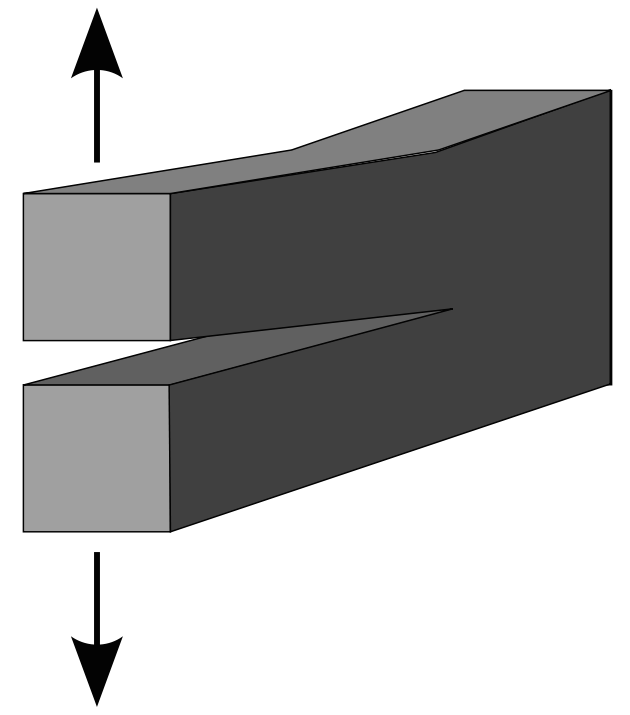
\includegraphics[width=\columnwidth]{IMG_CUTRES/wikipedia_failure_modes_1}
			Mode I:	Opening
\end{minipage}
\hfill
\begin{minipage}[b]{.3\columnwidth}
	\centering
	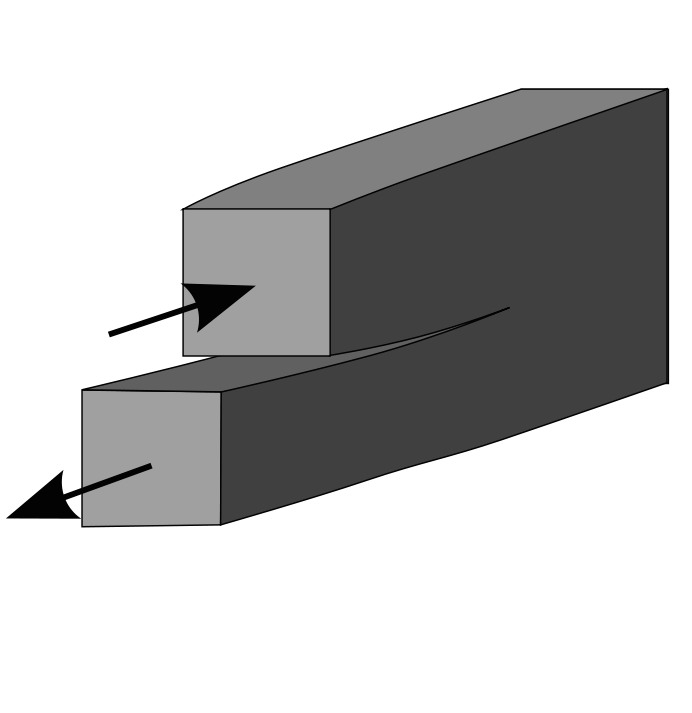
\includegraphics[width=\columnwidth]{IMG_CUTRES/wikipedia_failure_modes_2}
			Mode II: Sliding shear
\end{minipage}
\hfill
\begin{minipage}[b]{.3\columnwidth}
	\centering
	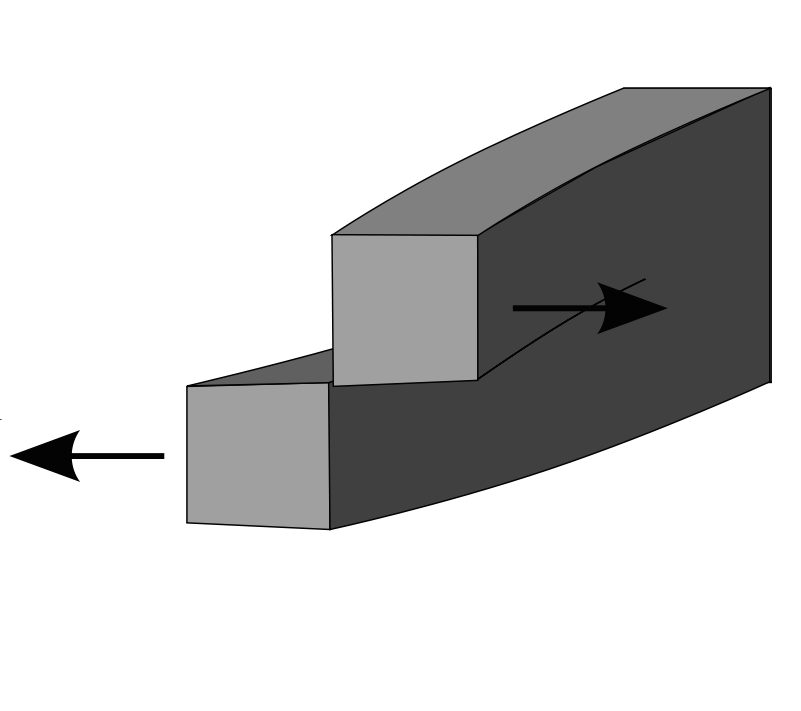
\includegraphics[width=\columnwidth]{IMG_CUTRES/wikipedia_failure_modes_3}
			Mode III: Tearing shear
\end{minipage}
	\caption[Schematic view of the three failure modes.]{Schematic view of the three failure modes. Taken from \citep{wiki_fracture_modes}.}
	\label{fig:wikipedia_failure_modes}
\end{figure}

\Gls{XFEM}-based \gls{LEFM} require a pre-existing crack in the model or some nucleation formulation that governs its propagation \citep{Abaqus613Manual}. As the crack's initial localization and direction is not previously known, the \gls{VCCT} criterion is used, which consists on correlating the displacement energy to the suffered damage. This technique can be applied in brittle crack formation, which is the case, as no plastification happens before damage or failure.

For this particular case, the \gls{VCCT} formulation was set as a fracture energy power law \citep{Loureiro2010, Sadowski2010, Sadowski2011, Sadowski2014, SernaMoreno2015}, as the given by \cref{eq:fracture_energy}.

\begin{equation}
\left(\frac{G_{I}}{G_{Ic}}\right)^{\alpha}+\left(\frac{G_{II}}{G_{IIc}}\right)^{\alpha}+\left(\frac{G_{III}}{G_{IIIc}}\right)^{\alpha}=1 ;
\label{eq:fracture_energy}
\end{equation}
where $G_{Ic}$ corresponds to the critical fracture energy required to cause failure in mode I (out-of-plane direction), and being $G_{IIc}$ and $G_{IIIc}$ the values for mode II and III, respectively, which correspond to both shear directions. The critical fracture energy for the Loctite Hysol 9514 in the normal direction is $\SI{2028}{\J/\m^2}$ \citep{Scattina2011}. It was considered that the adhesive had no preferential directions for tangential failure, meaning $G_{IIc}$ was equal to $G_{IIIC}$, and being the fracture energy equal to $\SI{11853}{\J/\m^2}$ \citep{Scattina2011}. These values are also depicted in \cref{tab:ads_dmg_params}. The exponent $\alpha$ was considered equal to $\num{2}$ \citep{Loureiro2010, Sadowski2010, Sadowski2011, Sadowski2014, SernaMoreno2015}.

In addition, relating this equation to \cref{eq:quads} a stress increase in one mode ---initially suppossed on the limit just before damage progression--- provokes stiffness loss in every mode involved in \cref{eq:fracture_energy}.

Once damage has started, according to this model, fracture energy is released as damage progresses reducing material stiffness. If unloaded, the material would behave elastically again with degraded properties until damage criterion is accomplished again. \Cref{fig:damage_evo2D} illustrates this behaviour for a simplified 2D case.

\begin{figure}
	\centering
	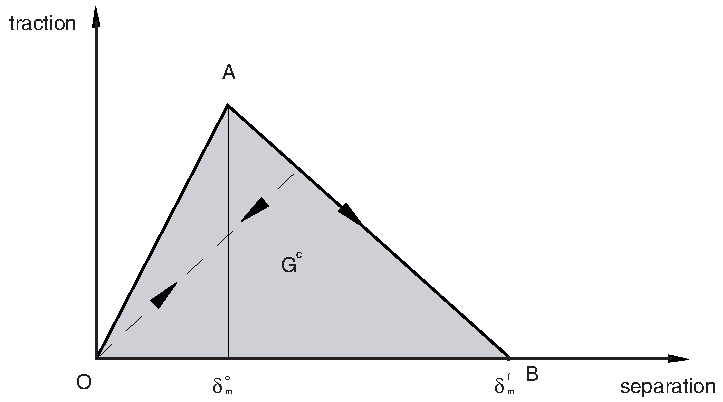
\includegraphics[width=0.7\linewidth]{IMG_CUTRES/damage_evolution_manual.pdf}
	\caption[Damage evolution representation for a 2D case.]{Damage evolution representation for a 2D case. Taken from \citep{Abaqus613Manual}.}
	\label{fig:damage_evo2D}
\end{figure}

Figure \ref{fig:damage} represents the whole damage model, including damage initiation and the fracture energy, which corresponds to the area beneath the curve.

\begin{figure}
	\centering
	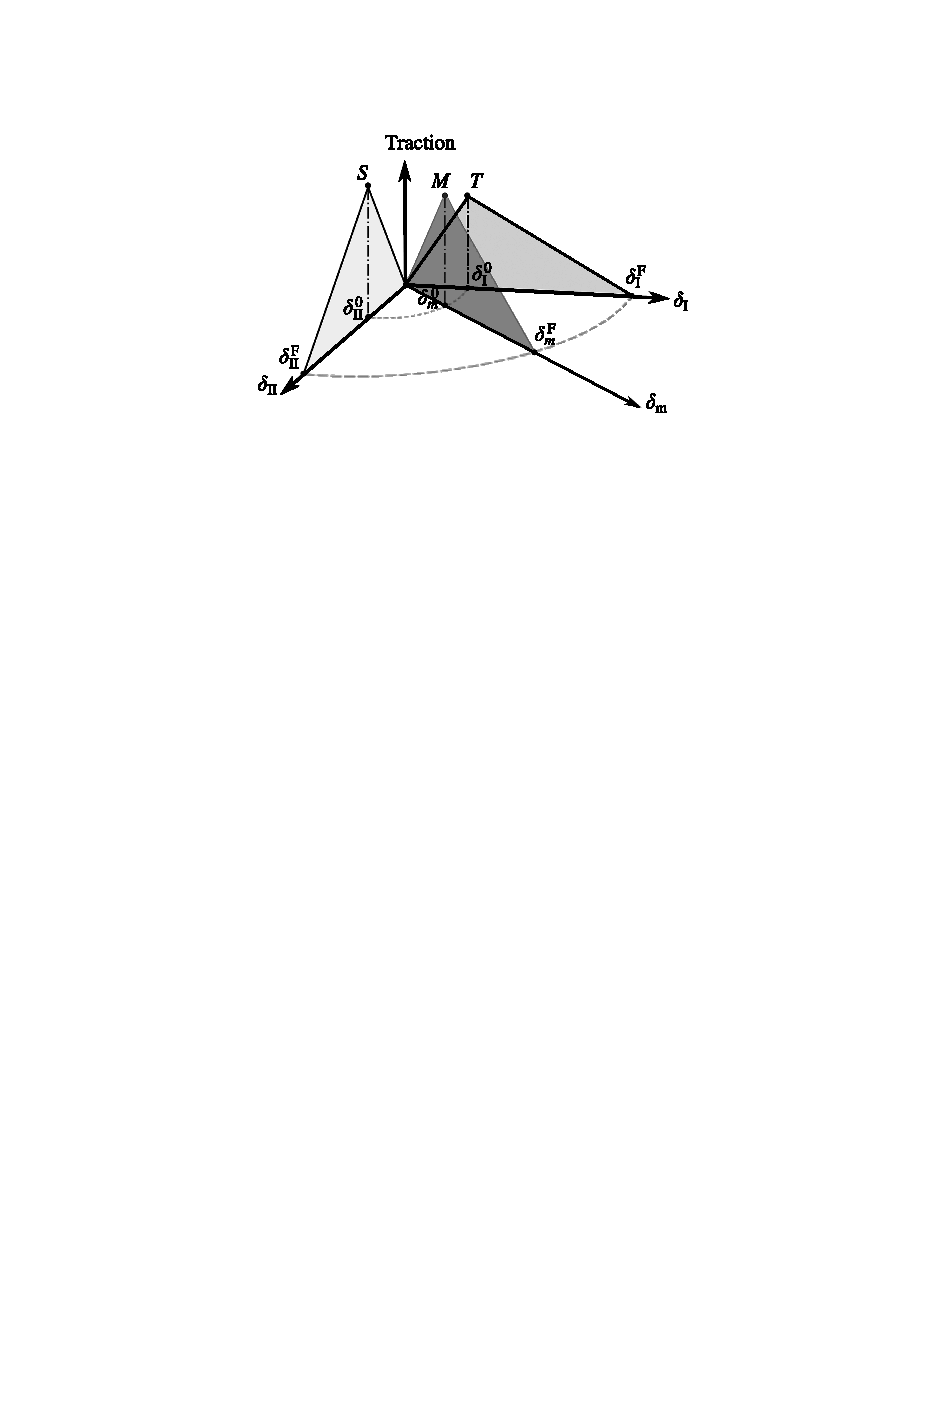
\includegraphics[width=0.7\linewidth]{IMG_CUTRES/scattina_quads}
	\caption[Damage model representation.]{Damage model representation. Traction represents the load; $\delta$, the displacement ($\varepsilon$ in this study); $S$ and $T$, the maximum load in two different modes ($\sigma_{n}^{0}$, $\tau_{II}^{0}$ or $\tau_{III}^{0}$), corresponding to damage initiation, which takes place at $\delta^0$; and $\delta_m$, the displacement in the mixed-mode loading. Taken from \citet{Scattina2011}.}
	\label{fig:damage}
\end{figure}

\subsection{Adherends}

In order to make the model comparable to the experiments carried out by \citet{Peroni2009}, steel was chosen for the adherends. In the present study, it is defined as an isotropic elastic-plastic material, with a density of $\SI{7.85}{\tonne/\m^3}$.

The elastic branch of the adherend stress-strain curve is defined as linear, with an elastic modulus of $\SI{200}{\GPa}$ and a Poisson ratio of $\num{0.3}$. It is followed by a perfectly plastic branch starting at $\SI{190}{\MPa}$ up to $\SI{1140}{\MPa}$, which is considered total failure of this material. This way, some strain is allowed during the plastic branch in order to avoid numerical issues, as it can be seen on \cref{fig:steel}.

\begin{figure}
	\centering
	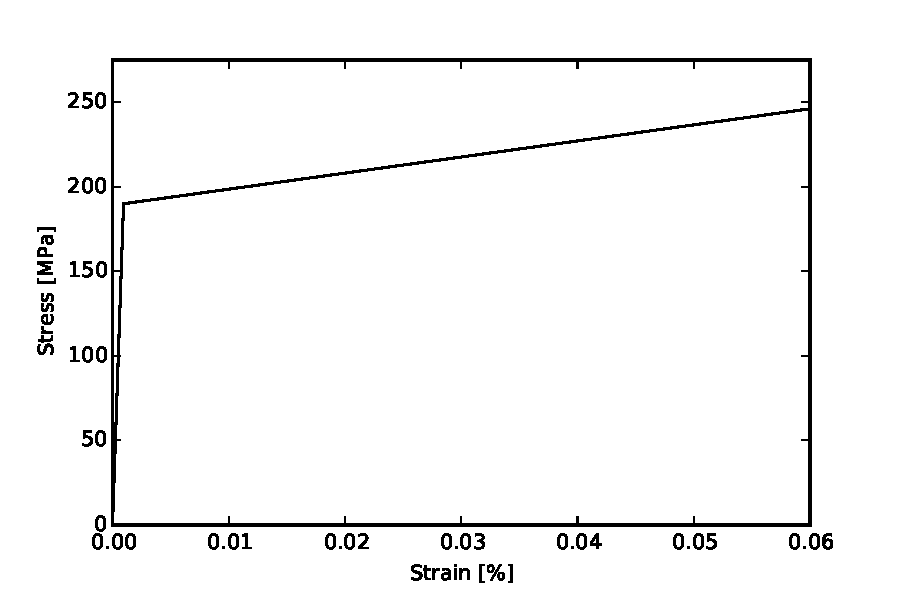
\includegraphics[width=0.7\linewidth]{IMG_CUTRES/steel}
	\caption{Steel stress-strain curve up to $\num{0.6}\text{\textperthousand}$ strain rate.}
	\label{fig:steel}
\end{figure}

It was supposed that the plastic branch of the steel would not develop enough to make necessary to take into account great kinematic harding effects, and was thus obviated.

\subsection{Interaction}

A general contact interaction was considered among all surfaces, including contact with themselves. Hard contact was considered on the normal direction, which implies that no penetration between surfaces may occur in case of contact. Models with both rough and frictionless contact were considered on the tangential directions, meaning that no slip may take place or that slip may happen without any resistance, respectively.

Frictionless models resembled those ones with penalty tangential behaviour with minor variations, specially on the last phases of the impact. This may be due to the absence of strong normal forces between adherends and with little tangential load. An exception is found in the tube end in contact with the impact plate, where tangential loading is more important, as the differences in the results point out.

\section{Computational and numerical considerations}
% Include computational time

\subsection{Hardware and software}

The finite element package Abaqus is used in this research, on is version 6.13 \citep{Abaqus613Manual} running on a high performance computing cluster running CentOS Linux distribution.

Abaqus calculation kernel ---Abaqus/Explicit in this case--- works parallelized on several processors in the cluster. Loop parallelization uses a shared memory paradigm and domain parallelization is based on a distributed memory model with message passing. \Gls{TcT} may vary between similar jobs depending on the processor capabilities. Due to this, only approximations to \gls{TcT} are given, instead of precise values.

Jobs running on loop parallelization over $16$ cores took about $\SI{8}{\hour}$ to finnish, which could be reduced to about $\SI{1}{\hour}$$\SI{15}{\minute}$ if mass scaling was applied. Domain paralelization turned out to be inefficient in this case due to network performance.


\subsection{Model parametrization}
\label{sec:script}

Excepting some details added in the last phases of the development of the present study, the whole model has been parametrized, making use of the Python interpreter integrated in Abaqus. This will allow model optimization in future phases of development. The parametrization code includes:

\begin{itemize}
	\item Geometrical parameters, including: tube length, bonding flanges dimension, adhesive and adherend thicknesses, among others.

	\item Impact conditions, such as speed or crush length.

	\item Two cross sections: square and hexagonal.

	\item Meshing parameters.

	\item Possibility to have a material library, although it is not used due to the lack of validated models.

	\item Optional tube fill with solid material and/or inner free plates.

	\item Different contact formulations.
\end{itemize}

A flowchart explaining the model creation process of the code is depicted in \cref{fig:flow}. The whole code can be seen in \cref{apx:script}. Complementary scripts were also developed for its work within the cluster and for its optimization using the Dakota optimization software package \citep{dakota}.

\begin{figure}
	\centering
	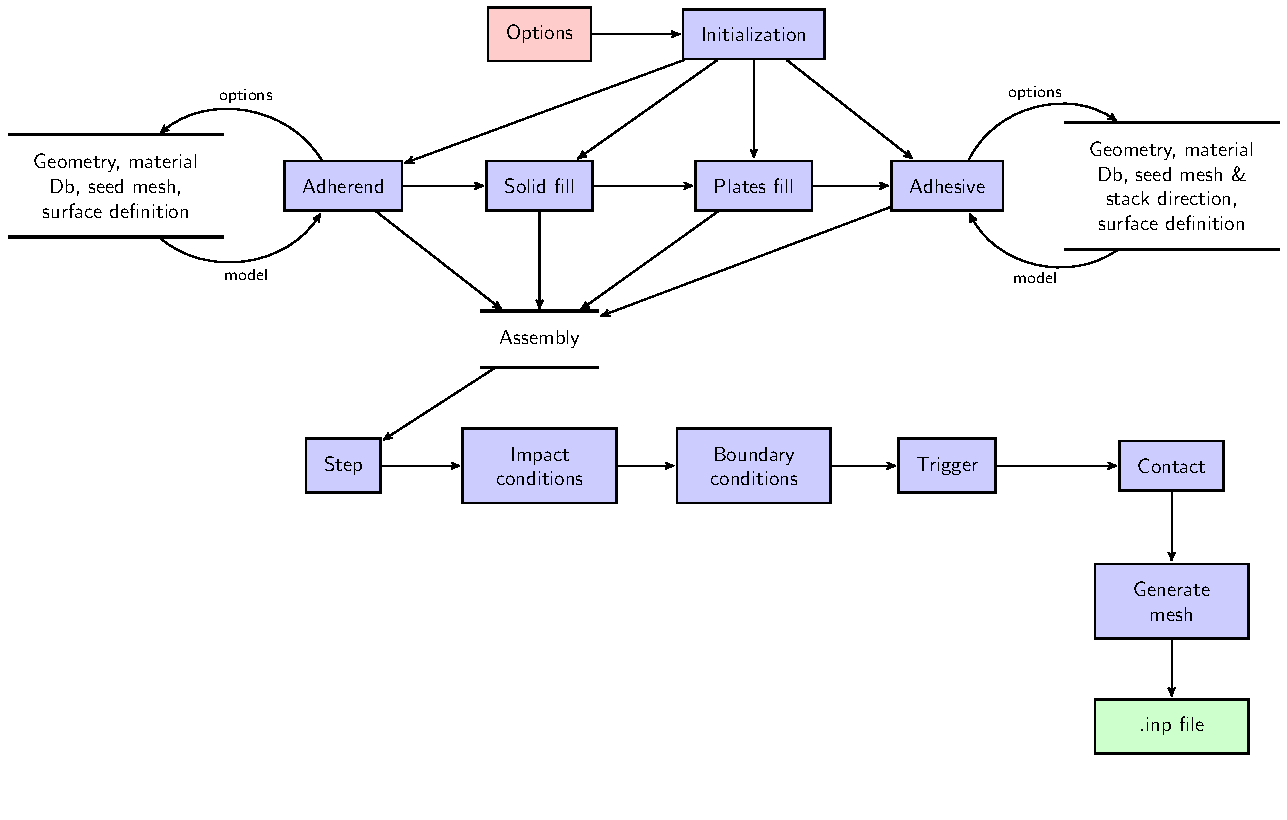
\includegraphics[width=.95\linewidth]{flowchart/flow}
	\caption[General structure of the parameterized code.]{General structure of the parametrization code. Straight arrows imply both chronological order and data dependency.}
	\label{fig:flow}
\end{figure}


\subsection{On the \acrlong{XFEM} and the explicit solver}
\label{sec:xfem}

The \gls{XFEM}, developed by \citet{Moes1999}, is a numerical technique based on the \gls{FEM} which enriches the solution in order to be able to work with discontinuities in the defining equations produced by material interfaces (named ``weak discontinuities'') or by a crack (named ``strong discontinuities'').

With this approach, errors in this discontinuities are alleviated at the same time that computational cost is reduced by eliminating the need of remeshing on the discontinuities. As a requirement for this method, these discontinuities can only happen on mesh edges.

Thanks to being based on the \gls{FEM}, it retains many of its advantages, outstanding the possibility of free geometries for the mesh.

Case of being a problem with time deffinition, a solver different from the standard has to be used. In the present study, Abaqus/Explicit was used as the solver. The tag ``Explicit'' points the method that is being used for the calculations.

Explicit methods are used in time-dependent problems and their implementation is based on:

\begin{equation}
S\left(t_{i+1}\right) = F_{i}\left(S\left(t_{i}\right)\right) ;
\label{eq:explicit}
\end{equation}
meaning that a state, $S$, at a certain time step, $t_{i+1}$, is calculated using the state at the previous time step, $t_{i}$. This method updates the stiffness matrix (included with other terms into $F$) after calculating each time step in order to take into account the effects of plastification, damage, etc.

In order to maintain a reasonable accuracy level, explicit methods require small time steps, although equilibrium of the structure with external forces is not granted within none of those steps.

Their counterpart are implicit methods, which solve the problem basing the state on a certain time step on that same state and on the previous one simultaneously through iterative methods, this is, including both states into $F$. Once convergence has been achieved, the following time step can be calculated.

They both have their limitations regarding to computational time ---being the implicit more computationally expensive--- and their aptitude to solve certain problems like cycling loads. The explicit method is used in the present study due to its aptitude for dynamic analysis.

\subsection{Finite element mesh}

The use of cohesive elements allowed to make the adhesive's mesh much coarser due to their aspect ratios requirements. These elements were created with a size of $\SI{2.0}{\mm}$, and had only one element in the $\SI{0.3}{\mm}$ layer thickness. Other tried element types, specifically solids, had problems if side lengths were bigger than about $\SI{0.5}{\mm}$, and were completely unfeasible with lengths larger than $\SI{1.0}{\mm}$ approximatedly.

% Tie (include image)
The tie constraint included in Abaqus allowed non-coherent meshes between adhesive and adherend (\cref{fig:mesh_detail_coh3d_comparison}). This way, finer meshes could be implemented on the adhesive in order to improve the representation of the failure progression without increasing the adherend element recount by leaving a coarser mesh there. If a structured mesh were used, a change on the adherend mesh on the union flanges would imply changing it in almost the whole adherend, in order to maintain the structured mesh.

\begin{figure}
	\centering
	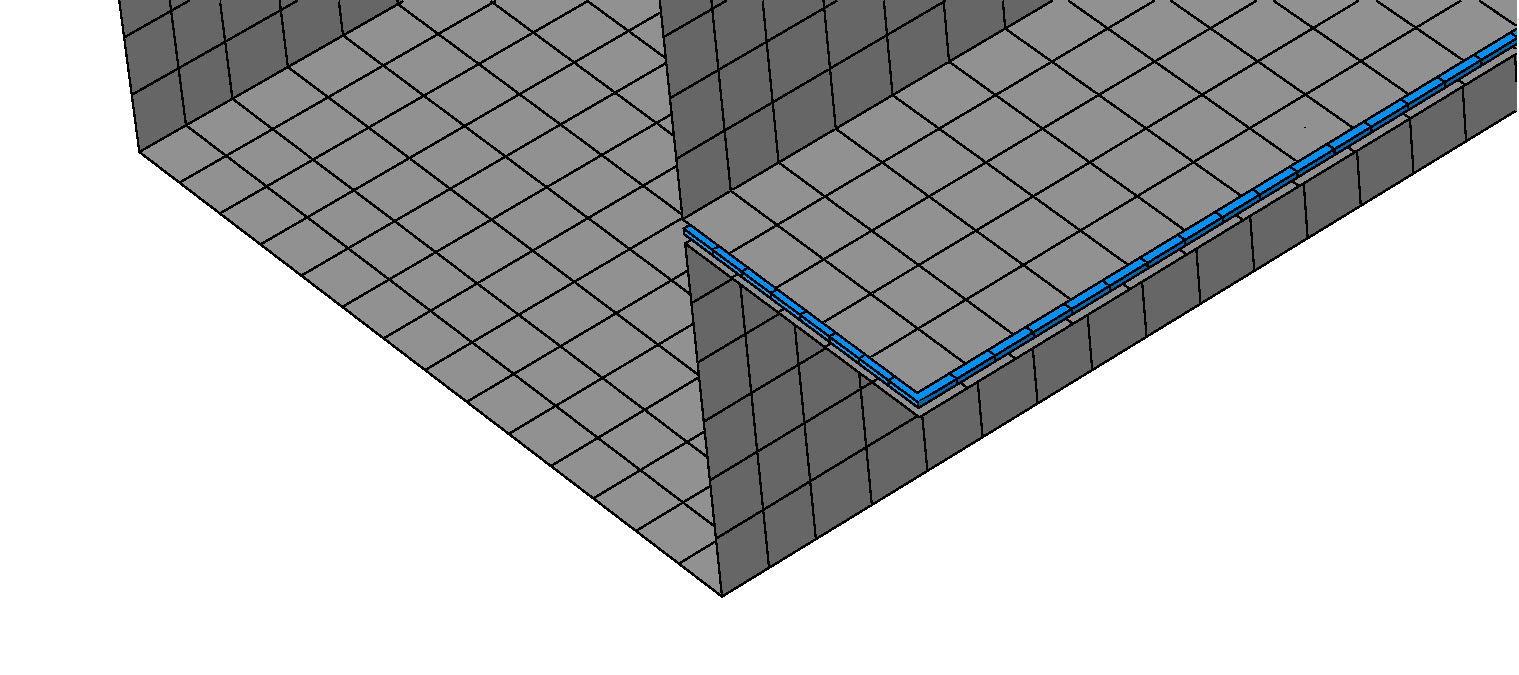
\includegraphics[width=0.7\linewidth]{IMG_CUTRES/mesh_detail_coh3d_comparison}
	\caption[Detail of \acrlong{COH3D} mesh on the adhesive layer.]{Detail of \acrlong{COH3D} mesh on the adhesive layer (blue).}
	\label{fig:mesh_detail_coh3d_comparison}
\end{figure}

% Mesh divisions for structure
Parts were partitioned, so a structured mesh could be applied in the most of the model, and limiting free meshes to the trigger surroundings. This detail is represented in \cref{fig:mesh_part}. It was firstly considered one of reasons for critical situations, and was performed aiming to relieve a possible numerical origin of these problems. Although it was eventually proven to not be related, it was finally maintained.

\begin{figure}
	\centering
	\begin{minipage}[b]{.48\linewidth}
		\centering
		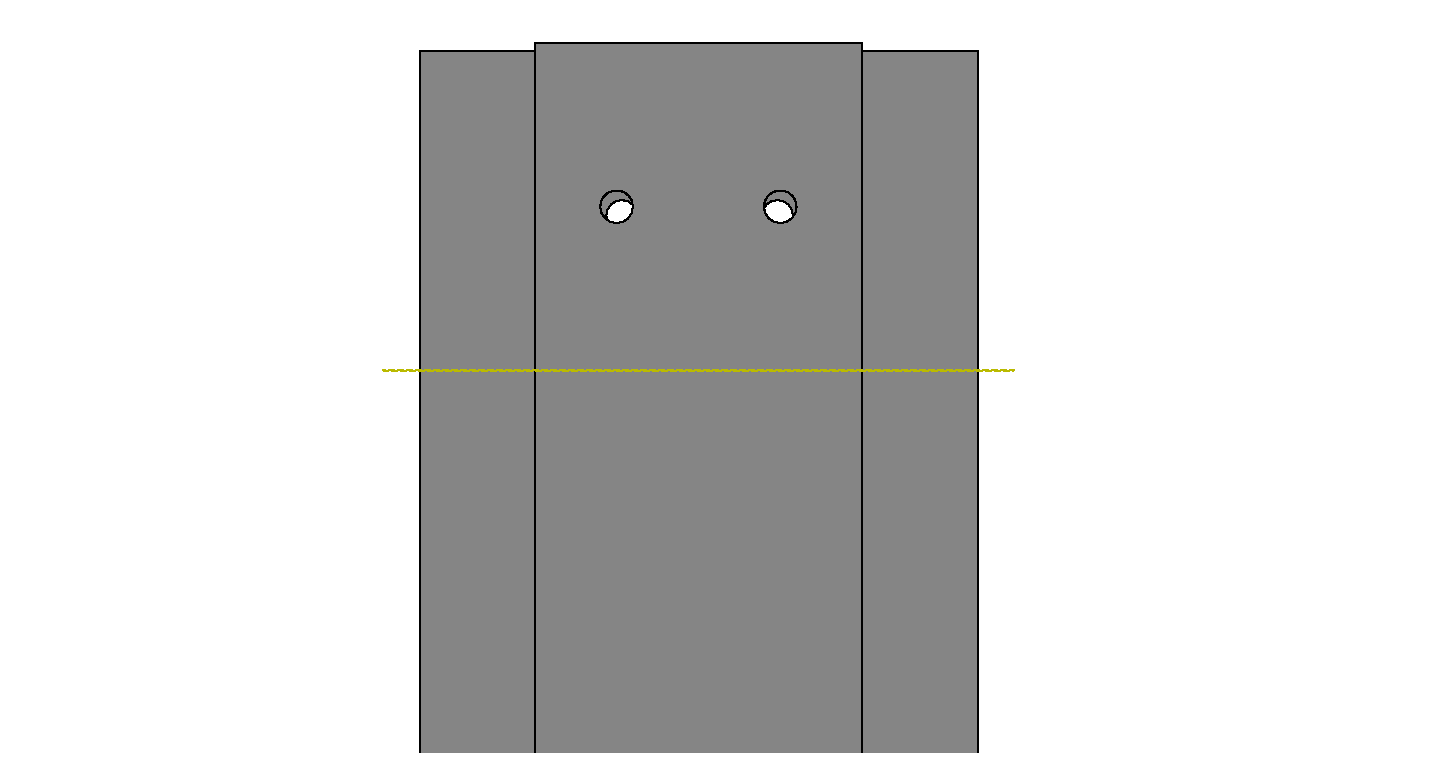
\includegraphics[width=\linewidth]{IMG_CUTRES/assembly_detail_holes}
	\end{minipage}
	\quad
	\begin{minipage}[b]{.48\linewidth}
		\centering
		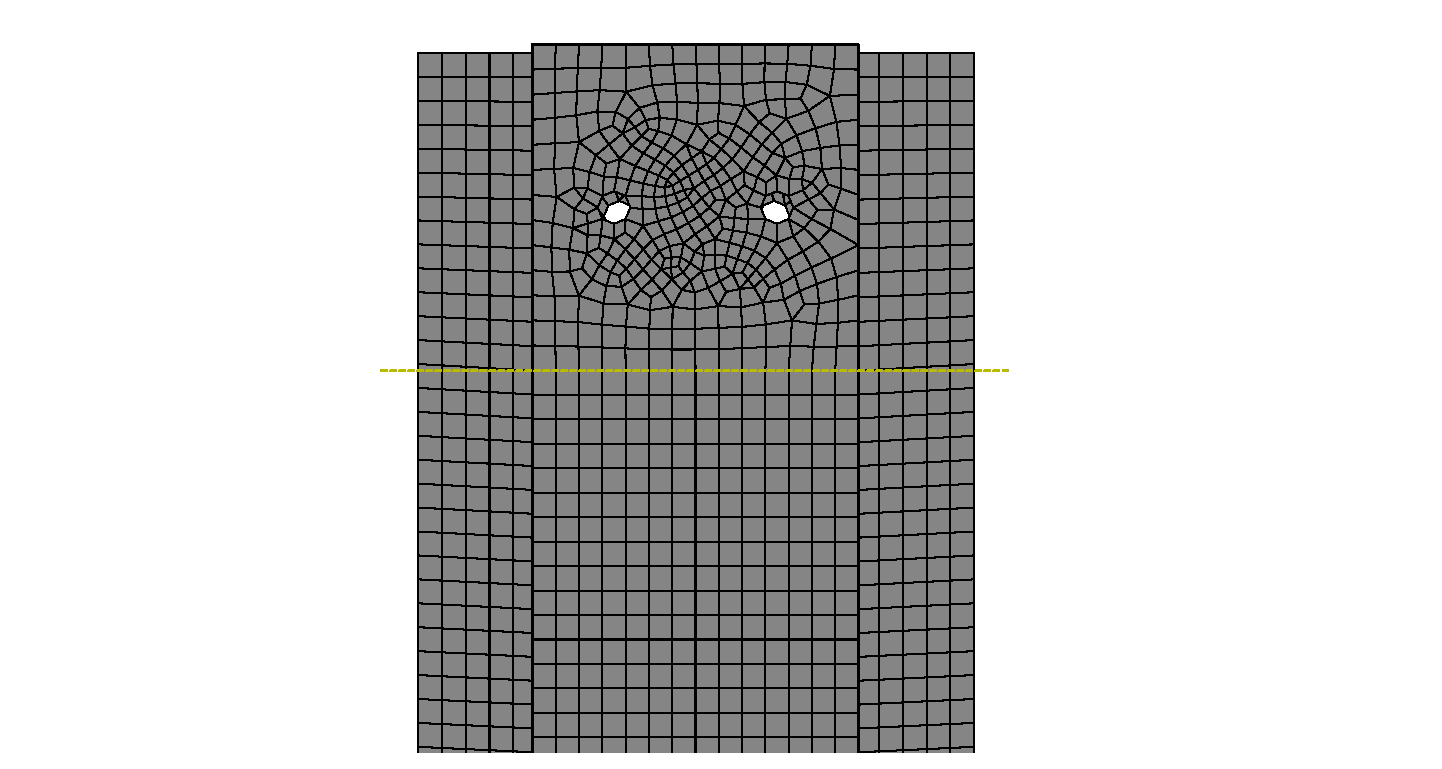
\includegraphics[width=\linewidth]{IMG_CUTRES/mesh_detail_holes}
	\end{minipage}
\caption{Assembly partitions detail for mesh structuring.}
\label{fig:mesh_part}
\end{figure}

Finally, \cref{fig:mesh} shows the used mesh for the crash tube, which has more than $\num{10600}$ elements, as \cref{tab:mesh} summarizes. In that same table, different element types are mentioned: ``S3'' and ``S4R'' are three and four noded general purpouse shell elements for structural analysis (the former one also includes reduced integration); ``R3D4'' are four noded 3D rigid quadrilateral; and ``COH3D'' are explained on \cref{sec:coh_elem}.

\begin{figure}
	\centering
	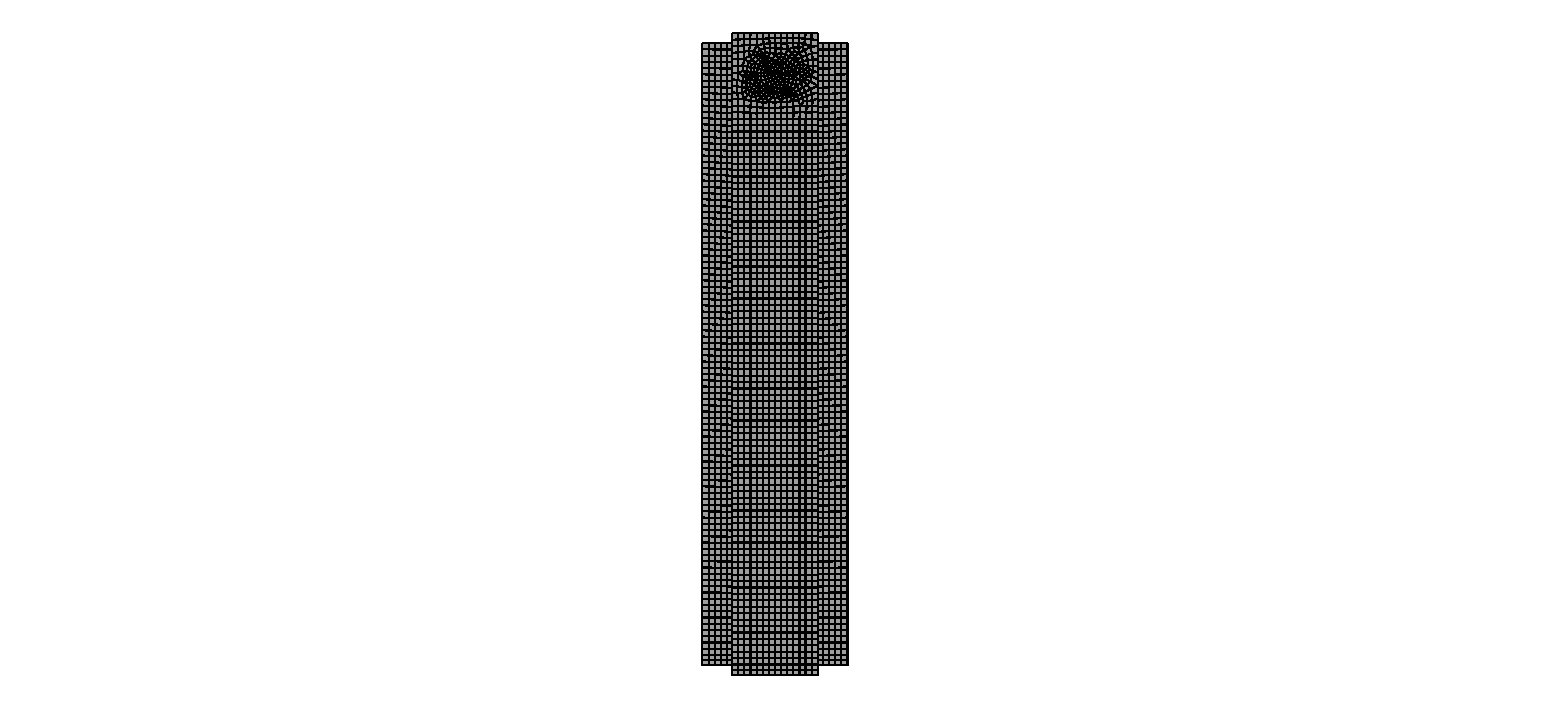
\includegraphics[width=0.9\linewidth]{IMG_CUTRES/mesh}
	\caption{General mesh of the crash box.}
	\label{fig:mesh}
\end{figure}

% Total recount of elements (by part?)
\begin{table}
	\centering
	\begin{tabular}{ll p{3cm} rr}

		\toprule

		Part & Element type & Mesh type & Elements & Nodes \\

		\midrule

		Adherend & S4R (S3) & Structured (with free partitions) & $3844$ ($33$) & $4010$ \\
		Adhesive & COH3D & Structured & $1200$ & $2718$ \\
		Rigid plates & R3D4 & Free & $10$ & $15$ \\
		Stabilizing box & R3D4 & Structured & $448$ & $480$ \\

		\midrule

		Total &&& $10622$ & $13966$ \\

		\bottomrule

	\end{tabular}
	\caption[Mesh summary.]{Mesh summary. Given values correspond to each instance of that part. In the adherend case, there is a seven element recount difference between each instance, probably due to the free mesh control in some partitions. The average value is given.}
	\label{tab:mesh}
\end{table}

\subsubsection{Mass scaling}
\label{sec:mass_scaling}

As \citet{Hale} explains, in explicit dynamic modelling, the total running time depends both on the model size (mesh size and total modelled time span) and in the time step size (${\Delta}t$). \Acrfull{SDT} is the maximum time step that still grants the numerical stability of the calculations, by supressing the possibility to a mechanical stress wave to go through more than one element in each time step. This condition is known as the Courant condition:

\begin{equation}
{\Delta}t_{stable} \leq f \left[\frac{h}{c}\right]_{min} ;
\label{eq:courant}
\end{equation}
where $f$ is a factor, usually $0.9$; $h$ is the element dimension; and $c$ is the wave speed in that same element; the minimum is calculated within the whole model. The wave speed can be calculated as

\begin{equation}
c = \sqrt{\frac{E}{\rho}} ;
\label{eq:wave_speed}
\end{equation}
where $E$ is the Young modulus; and $\rho$, the density. Among the values expresed in \cref{eq:courant,eq:wave_speed}, only density can be modified without heavily affecting accuracy. Applying this in order to improve numerical performance of the model is known as mass scaling.

Software packages calculation kernels usually include this feature applying it selectively to those elements which are determining the unfavorable \gls{SDT} in each time step.

Following \citet{Scattina2011}, mass scaling was applied to the adhesive's density in the whole model, that is, with a given selection of element which corresponds to all adhesive elements.

Increasing it one order of magnitude results on a \gls{SDT} up to 30 times bigger. Increasing it two orders of magnitude results in very similar improvements, a bit worse perhaps. A factor of 40 was finally used, resulting in a \gls{SDT} almost two orders of magnitude bigger than the original ones.

\subsubsection{The \acrlong{COH3D}}
\label{sec:coh_elem}

As \acrlong{COH3D} were specifically formulated for adhesive modelling, among other uses, they have been widely used to model this material, in Abaqus \citep{Sadowski2010, Sadowski2011, Sadowski2014, Alvarez2014} and in other software packages \citep{Sato2000, Carlberger2007, Loureiro2010, Scattina2011, Ghasemnejad2013}, although this is not the only existing formulation \citep{Sato2000, Greve2007, Liao2011, Yang2012}. Certain stress distributions cannot be properly modelled, such as in-plane compression, but these have no interest or negligible effects. In Abaqus, these elements are denominated \acrshort{COH3D} and require that:
\begin{itemize}
	\item There can only be a single layer of elements.

	\item Element's shape must be plate-like: height smaller than the other dimensions, but not negligible.

	\item A stack direction, usually based on the first point, and represented by $x'_{2}$ in \cref{fig:coh3d_csys}, in order to define the direction of the traction loading.
\end{itemize}

As the adhesive layer is very thin, it matches this geometrical requirements, making these elements suitable for this application (see \cref{fig:mesh_detail_coh3d_comparison}). These needed aspect ratios allow a coarser mesh on this part, if compared to general purpouse 3D elements, with access to better-fit formulations, and thus good results.

\begin{figure}
	\centering
	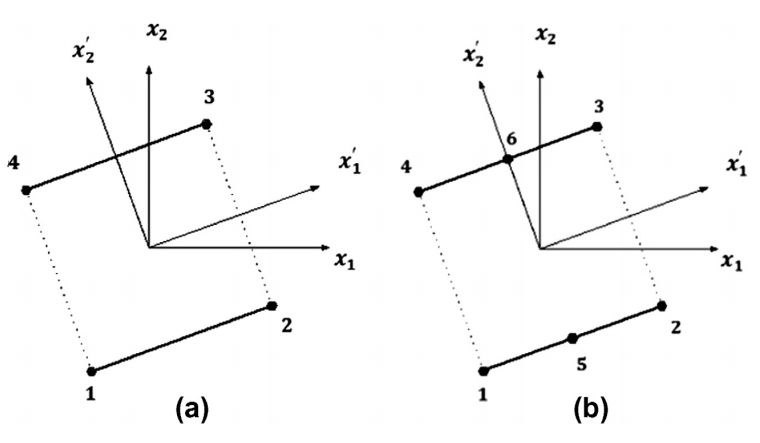
\includegraphics[width=0.7\linewidth]{IMG_CUTRES/coh3d_csys}
	\caption[Representation of linear and cuadratic cohesive 2D elements.]{Representation of linear (a) and cuadratic (b) cohesive 2D elements. Axis denoted as $x_{i}$ are refered to the global coordinate system, being the $x'_{i}$ in the local coordinate system. In this case, $x'_{1}$ is the in-plane axis, and $x'_{2}$ is the normal axis, paralell to stack direction. Taken from \citet{Alvarez2014}.}
	\label{fig:coh3d_csys}
\end{figure}

\Glspl{COH3D} with the same element length as the adherend elements could be used without computational problems. But a such coarse mesh showed some difficulties on modelling damage behaviour, depicting a too staggered failure, instead of being more continuous-like.

\begin{figure}
\centering
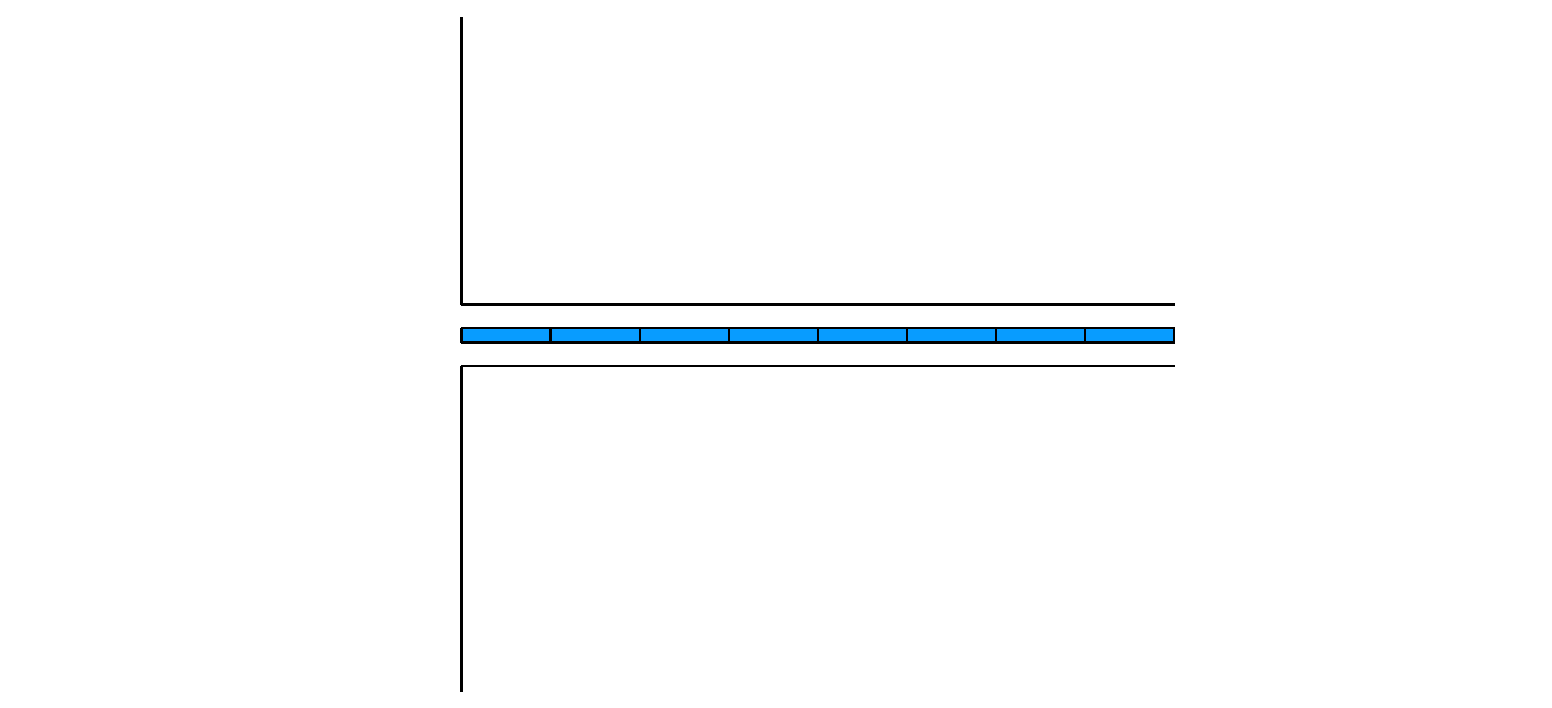
\includegraphics[width=0.7\linewidth]{IMG_CUTRES/ads_detail}
\caption{Frontal detail of the adhesive layer elements.}
\label{fig:ads_detail}
\end{figure}

Although the quadratic nominal stress criterion formulation exists as a bulk damage model and as a contact damage model, only the former one was used. Using both would have been more realistic \citep{Wu2013}, but it brought simulation problems: elements separating alternatively from each adherend appeared together with elements inbetween in good state. Instead of getting stiffness degradation in the whole adhesive, undamaged elements were here subjected to the load their neighbours weren't handling, and thus failing significantly reducing adhesive's overall resistance, apart from other numerical issues.

The contact interaction was eventually substituted by a tie constraint between the \glspl{COH3D} surface and the adherend elements (see \cref{fig:ads_detail} for in-model detail, and \cref{fig:union} for a schematic view of the concept). It is suppossed that the use of quadratic nominal stress criterion for contact interaction properties is more suitable for those cases in which the bulk of the adhesive layer is not of interest and the focus is on a general behaviour of the structure.

\begin{figure}
	\centering
	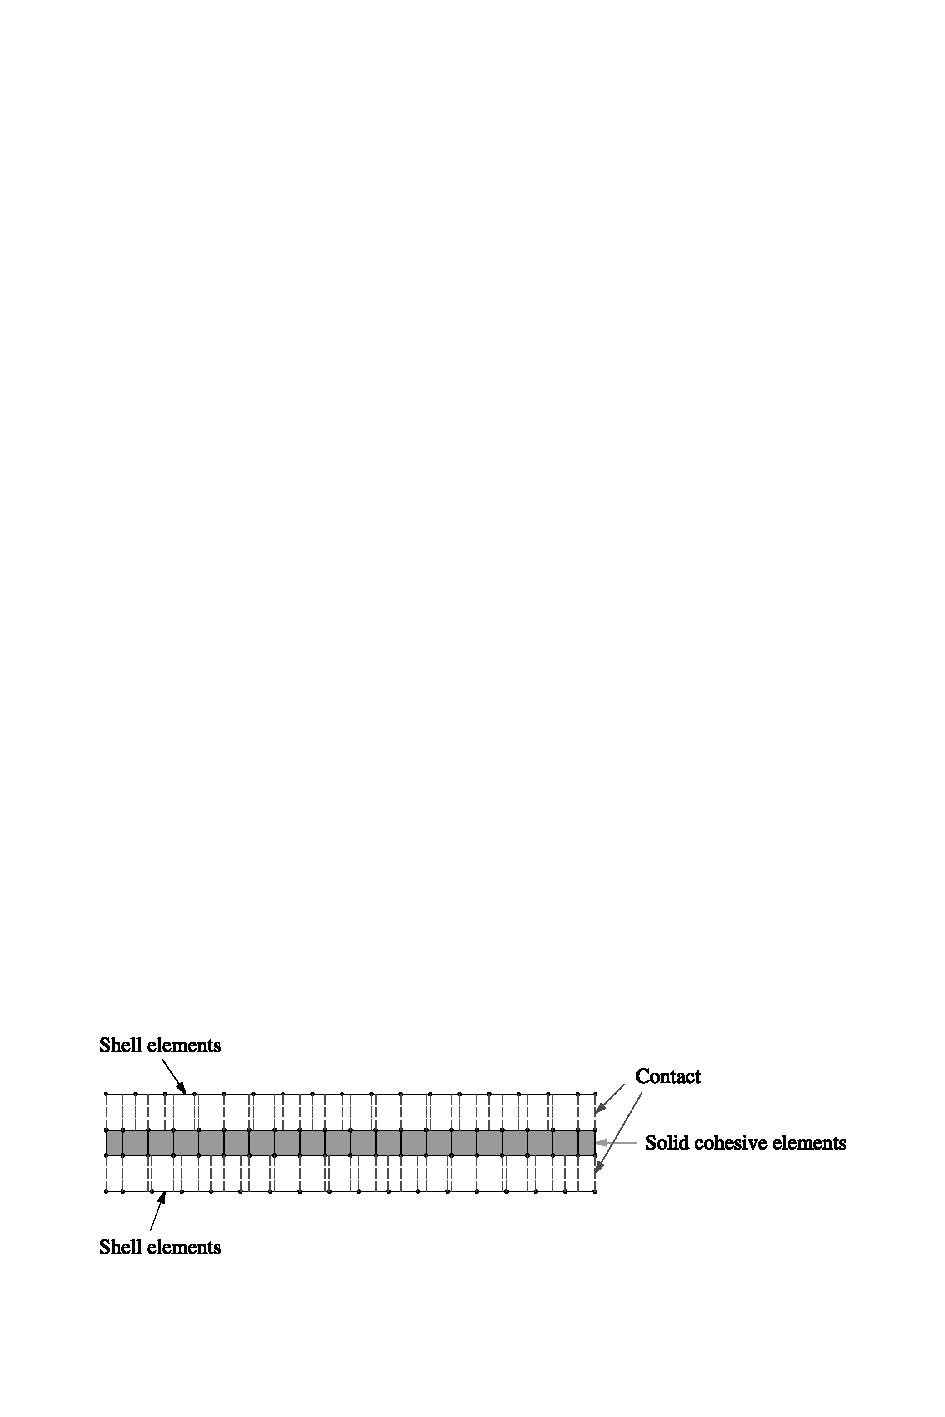
\includegraphics[width=0.7\linewidth]{IMG_CUTRES/union}
	\caption[Cross section detail of the adhesive layer modelled with \acrlongpl{COH3D} between two adherends modelled with shell elements.]{Cross section detail of the adhesive layer modelled with \acrlongpl{COH3D} between two adherends modelled with shell elements. Taken from \citet{Scattina2011}.}
	\label{fig:union}
\end{figure}

As the used damage model is a particular case of \gls{VCCT}, it can only be applied in certain element types, like the \gls{COH3D}. It supposes a formulation that strongly penalizes the minimum \gls{SDT} \citep{Abaqus613Manual}, reducing it even to the order of $\SI{1.5e-9}{\s}$, much more unfavorable if compared to other damage models tried during the development of this study, which made it about $\SI{2e-7}{\s}$.

It is recommended to see the work done by \citet{Alfano2001} for a deeper explanation on the \gls{COH3D} element formulation, and the article written by \citet{May2014} for deeper information on failure formulations.

\chapter{Results and discussion}
\label{results}

\section{Measurement and validation}

\subsection{\Acrlong{Ea}}  % Integration of Force/Disp curves
\label{sec:Ea}

As previously stated, one of the main purpouses of the studied devices is to absorb the biggest amount of energy on an impact.

The total amount of dissipated energy, \gls{Ea}, by whichever mechanisms, will be equal to the total input energy. Therefore, \gls{Ea} would, ideally, be the result of integrating the force-displacement curve during the deformation, as indicated in \cref{eq:Ea_concept}.

\begin{equation}
E_a = \int_{s_0}^{s_f} F(s) \mathrm{d}s ;
\label{eq:Ea_concept}
\end{equation}
where $s$ is the displacement; $s_0$ and $s_f$ are the initial and final displacements of the impact plate respect to a certain reference; and $F(s)$ is the force for that differential increment of displacement. \Cref{eq:Ea_approx} is an adaptation of \cref{eq:Ea_concept} that is used in this study.

\begin{equation}
E_a \approx \displaystyle\sum_{i=0}^{N-1} \frac{F_{i+1}^R+F_{i}^R}{2} \left(s_{i+1}-s_{i}\right) ;
\label{eq:Ea_approx}
\end{equation}
where $N$ is the total amount of output steps. The superindex $R$ affecting the force term stands for ``rear'', as its measured in the rear plate in order to prevent too much noise in the output.

\Acrfull{SEA}, as an output parameter, consists on \gls{Ea} normalized to the mass of the crash box, and it is also used to validate the model, together with \acrfull{F-D}, by comparing the obtained values with those obtained by \citet{Peroni2009}. Although some differences may appear, their origin is in the discrepancies on \gls{F-D}.

\subsection{\Acrlong{F-D}}
\label{sec:F-D}

Typical crash test \acrlongpl{F-D} present a series of alternating peaks and valleys of similar values, except for the first peak, which is greater in value (about twice or three times the mean value) and much more pronounced, as it can be seen on \cref{fig:phdcostas_f-d}. Except in case of critical situations, a clear maximum peak takes place in this first peak.

\begin{figure}
\centering
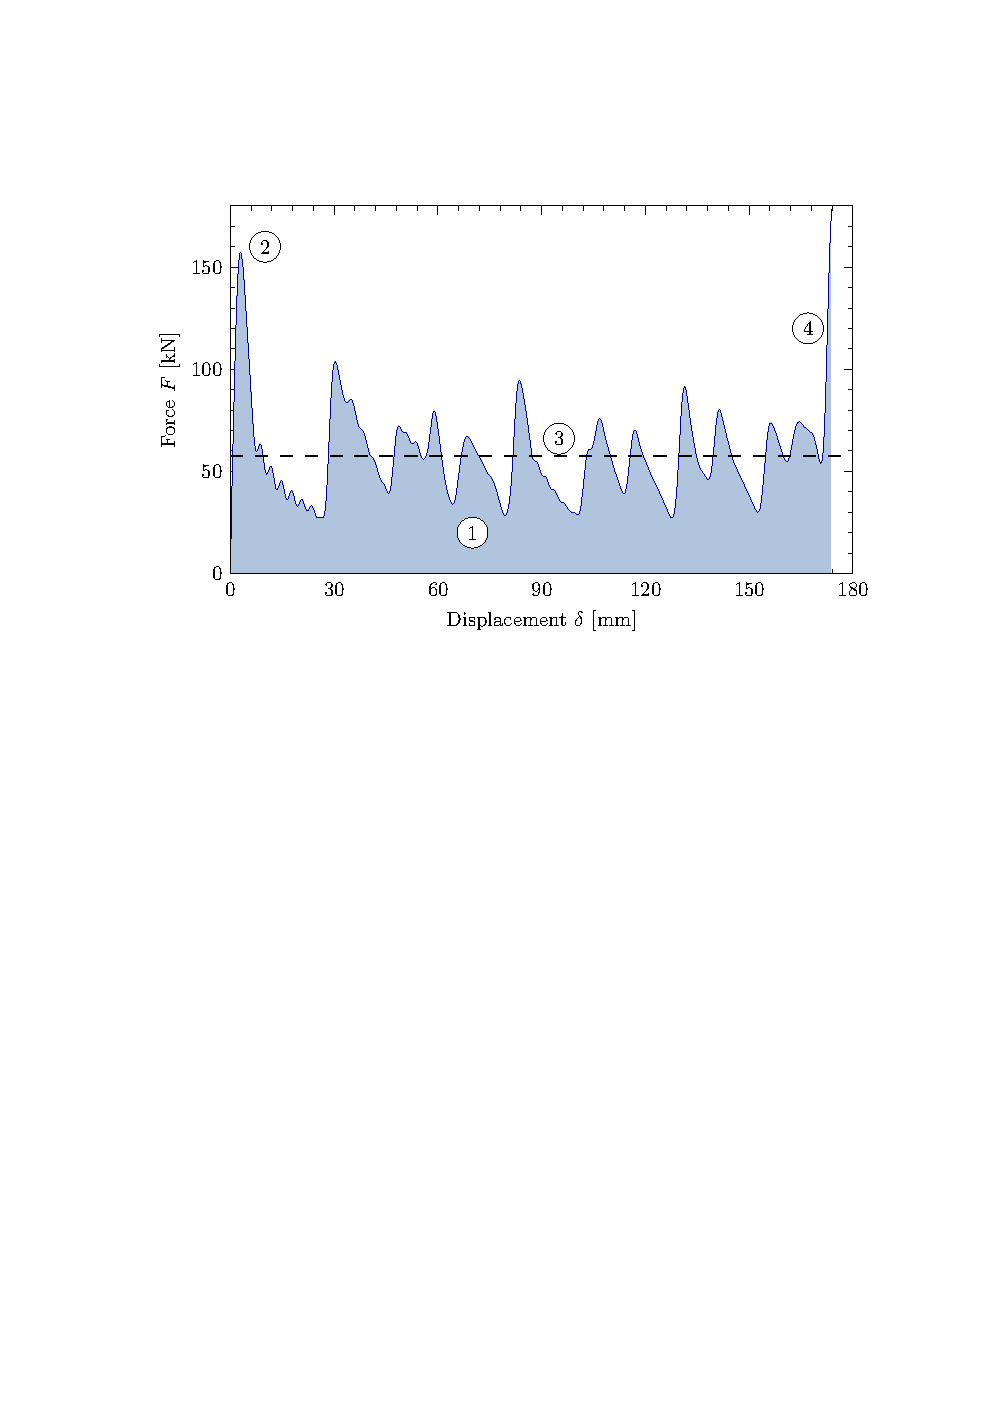
\includegraphics[width=0.7\linewidth]{./IMG_CUTRES/phdcostas_f-d}
\caption[Another \acrlong{F-D}.]{Another \acrlong{F-D}. Taken from \citet{phdCostas}.}
\label{fig:phdcostas_f-d}
\end{figure}

In order to filter high frequency effects, a SAE 600 filter was applied to the simulation results \citep{Huang}. This was also interesting as the level of noise in the output functions made it difficult to distinguish them when plotted together. \Cref{fig:F-D_frictionless,fig:F-D_rough} display modelled crash boxes with frictionless and rough interaction properties respectively. In that same figure and in the upcoming ones, nomenclature is as follows:

\begin{itemize}
	\item ``A'' or ``B'' indicating the cross-section of the tube: ``A'' for the top-hat, and ``B'' for the double hat.

	\item Following that, ``R'', indicating that the rough tangential contact property was used, or ``Fl'', for the frictionless case.

	\item An ``R'' after the underline indicates that the crash box had riveting in the triggered cross section.

	\item ``Sb'' after the underline marks the presence of a stabilizing box in the model.
\end{itemize}

% Insert obtained F-D curve
\begin{figure}
	\centering
	\begin{minipage}[b]{.9\linewidth}
		\centering
		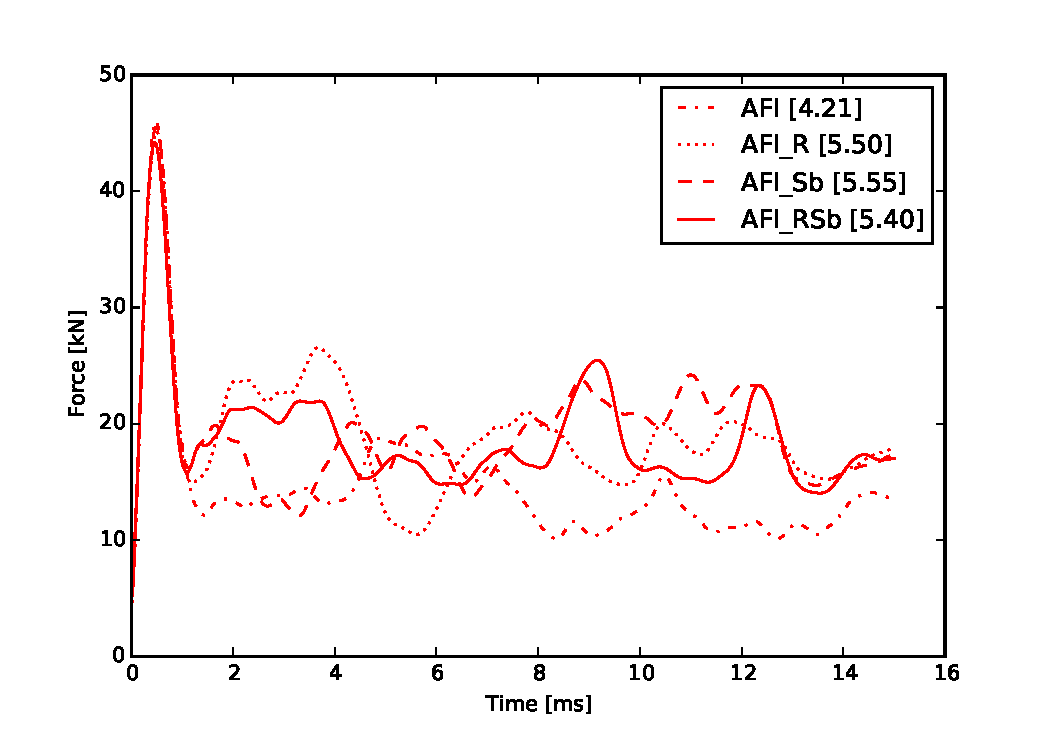
\includegraphics[width=\linewidth]{IMG_CUTRES/AFl}
	\end{minipage}
	\quad
	\begin{minipage}[b]{.9\linewidth}
		\centering
		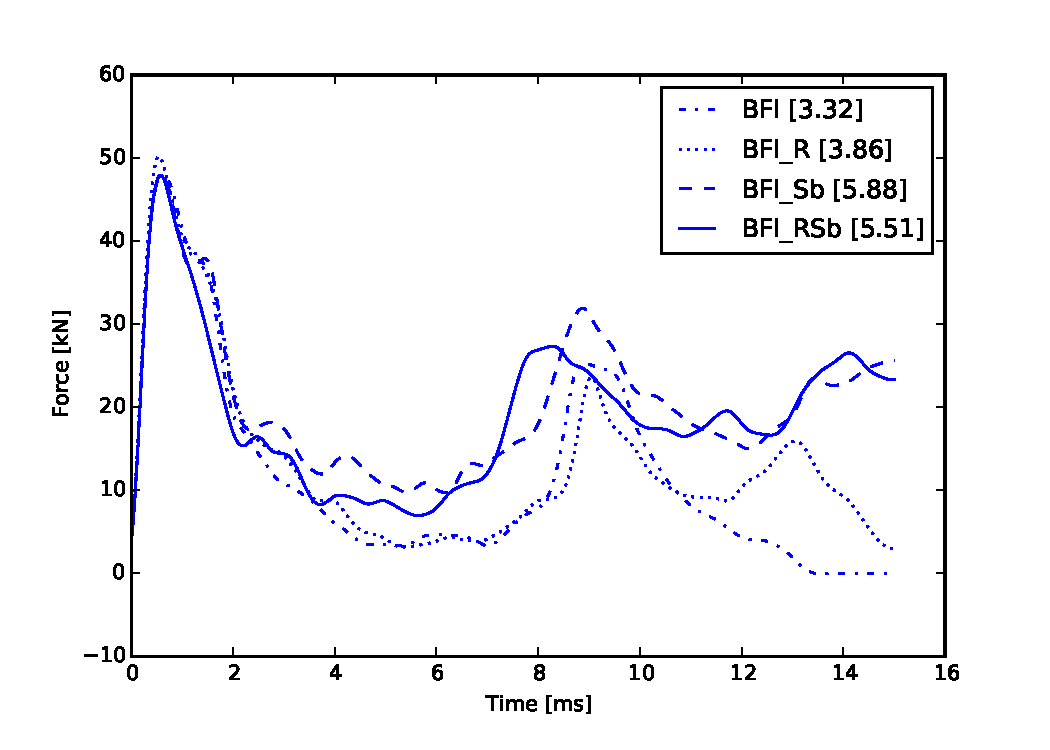
\includegraphics[width=\linewidth]{IMG_CUTRES/BFl}
	\end{minipage}
	\caption[\Acrlongpl{F-D} for modelled cross sections, both top-hat and double hat, with different modelled configurations with frictionless contact.]{\Acrlongpl{F-D} for modelled cross sections, both top-hat (red) and double hat (blue), with different modelled configurations with frictionless contact. \Gls{SEA} values in brackets in $\si{\kJ/\kg}$.}
	\label{fig:F-D_frictionless}
\end{figure}

\begin{figure}
	\centering
	\begin{minipage}[b]{.9\linewidth}
		\centering
		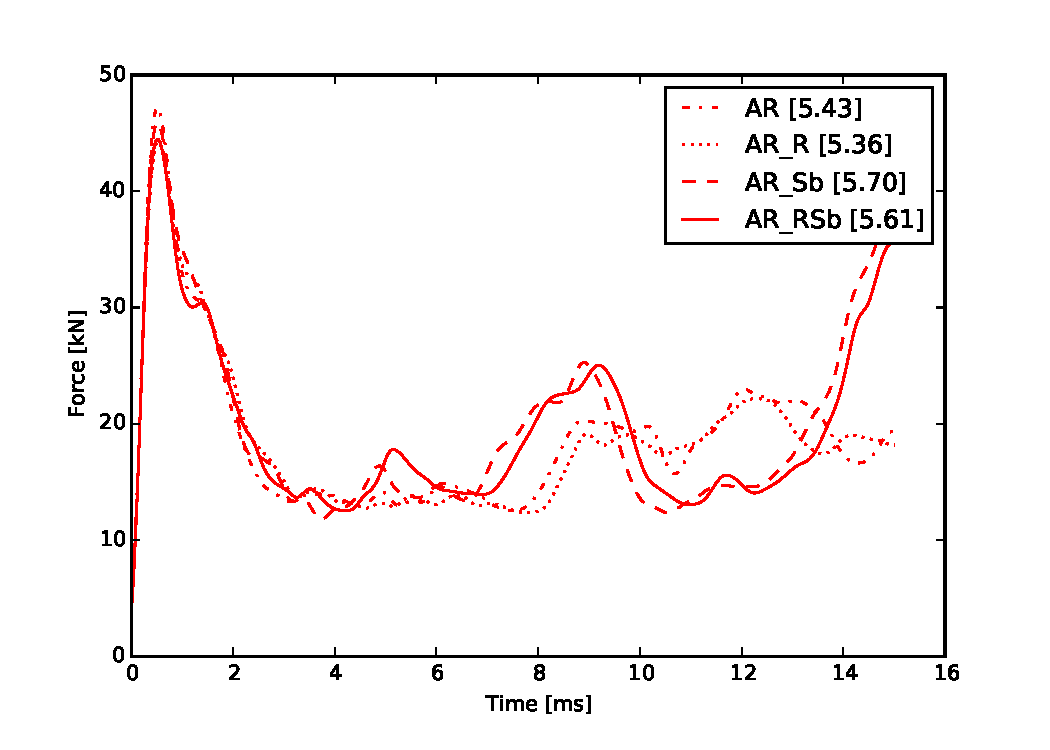
\includegraphics[width=\linewidth]{IMG_CUTRES/AR}
	\end{minipage}
	\quad
	\begin{minipage}[b]{.9\linewidth}
		\centering
		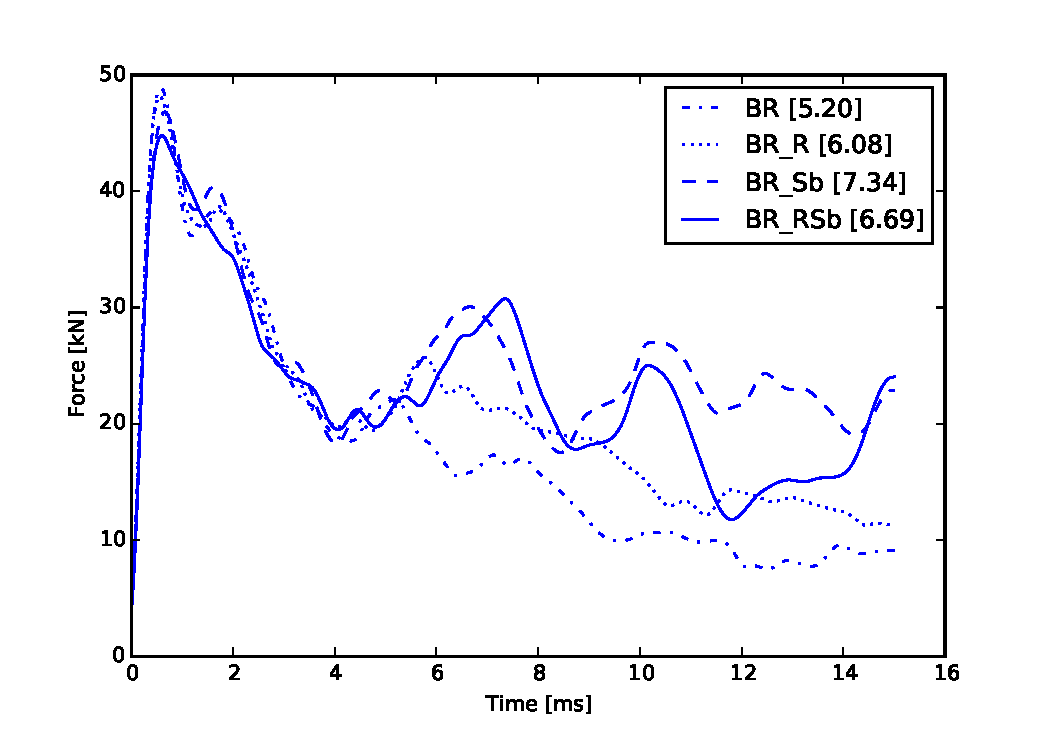
\includegraphics[width=\linewidth]{IMG_CUTRES/BR}
	\end{minipage}
	\caption[\Acrlongpl{F-D} for modelled cross sections, both top-hat and double hat, with different modelled configurations with rough contact.]{\Acrlongpl{F-D} for modelled cross sections, both top-hat (red) and double hat (blue), with different modelled configurations with rough contact. \Gls{SEA} values in brackets in $\si{\kJ/\kg}$.}
	\label{fig:F-D_rough}
\end{figure}

\begin{figure}
	\centering
	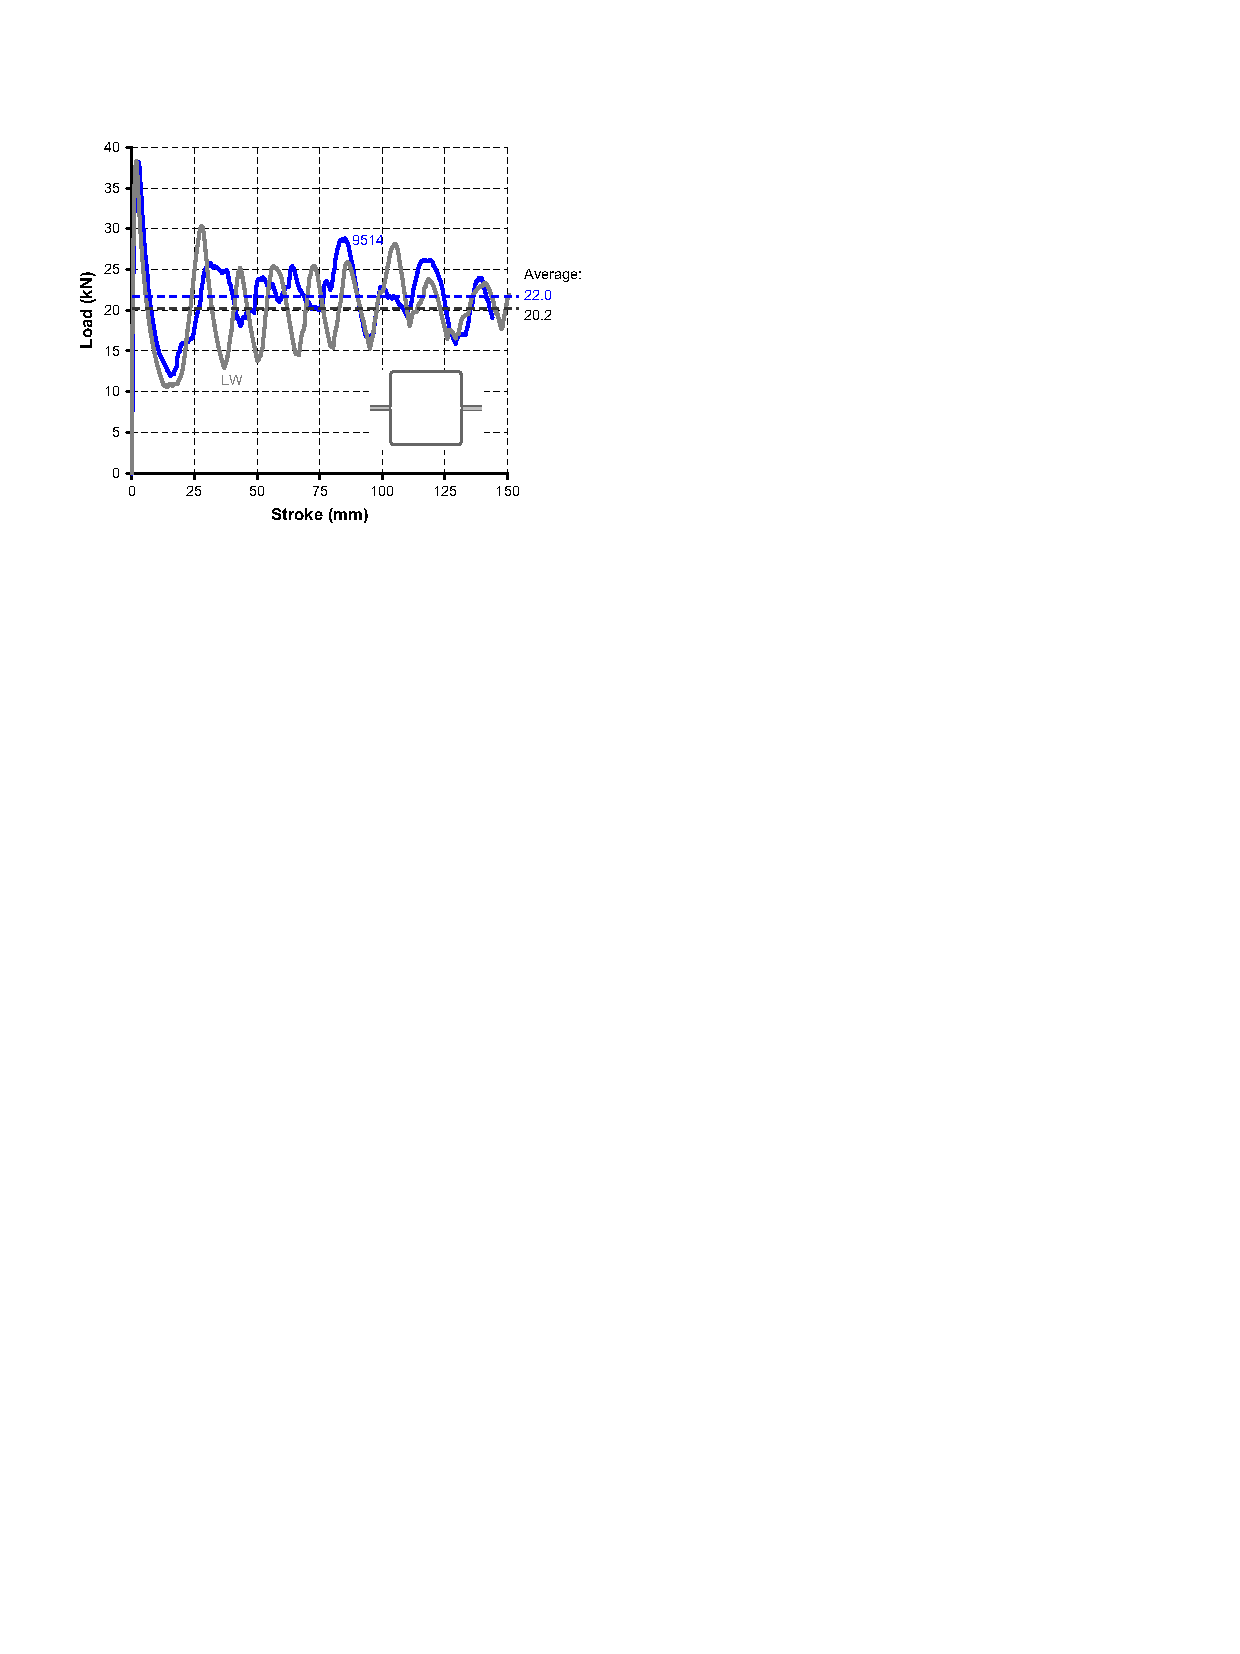
\includegraphics[width=0.7\linewidth]{IMG_CUTRES/peroni_qstat_fd}
	\caption[\Acrlong{F-D} obtained by \citet{Peroni2009} in quasi-static test for studied adhesive and other bonding solution.]{\Acrlong{F-D} obtained by \citet{Peroni2009} in quasi-static test for studied adhesive (blue) and other bonding solution (grey).}
	\label{fig:peroni_qstat_fd}
\end{figure}

Qualitatively, this curves are very similar to those obtained by \citet{Peroni2009}. \Cref{fig:peroni_qstat_fd} depicts a quasi-static test performed by these authors with the same section and bonding solution. Facing these similitudes, the model is considered valid. Differences are commented on \cref{sec:interpretation}.

In general, a uniform \gls{F-D} would be the most desirable scenary, as it would imply maximizing the \gls{Ea} ---which would be equal to the average value multiplied by the total time--- with the minimum \gls{Pk}. As this is not possible in practice, the best solution will be the one with the most constant-like behaviour.

\subsubsection{Mean and standard deviation}

The mean and the \gls{SD} of \gls{F-D} are measured in each case. The former one is the least interesting of both, as it is directly related to \gls{SEA}, which is already being calculated.

However, \gls{SD} is fair more interesting for the analysis, as it gives an idea of the uniformity of the \gls{F-D} during the analysis time span. As high values of the transmitted force are origin of injury of the occupants, the most uniform resulting curve will be the one with the lesser values of local peaks for the same mean load, and thus, the more desirable.

\section{Collapse mechanism}

The origin of the mentioned difference between quasi-static and impact results may be related to the collapse mechanism. Specifically, to the rate of changing the response mechanism for the crash box, from in-plane compression of the plates ---which is directly related to \gls{Pk}---, to the initiation of wave formation. In the developed model, if compared to the collapse images provided by \citet{Scattina2011}, this rate is far slower. The last local peak of the \gls{F-D} does not take place within the simulation interval due to a longer time span of the main peak.

\subsection{Wave formation}
\label{sec:wave_formation}

Crash box plates bending is the main way of energy absorption through elastic-plastic deformation. Wave formation consists on the formation of a series of foldings along the plates of alternating directionality, so the geometric axis of the tube is approximatedly kept in place, as it can be seen on \cref{fig:waves}. The non-accomplishment of this last condition is a case of critical situation.

\begin{figure}
\centering
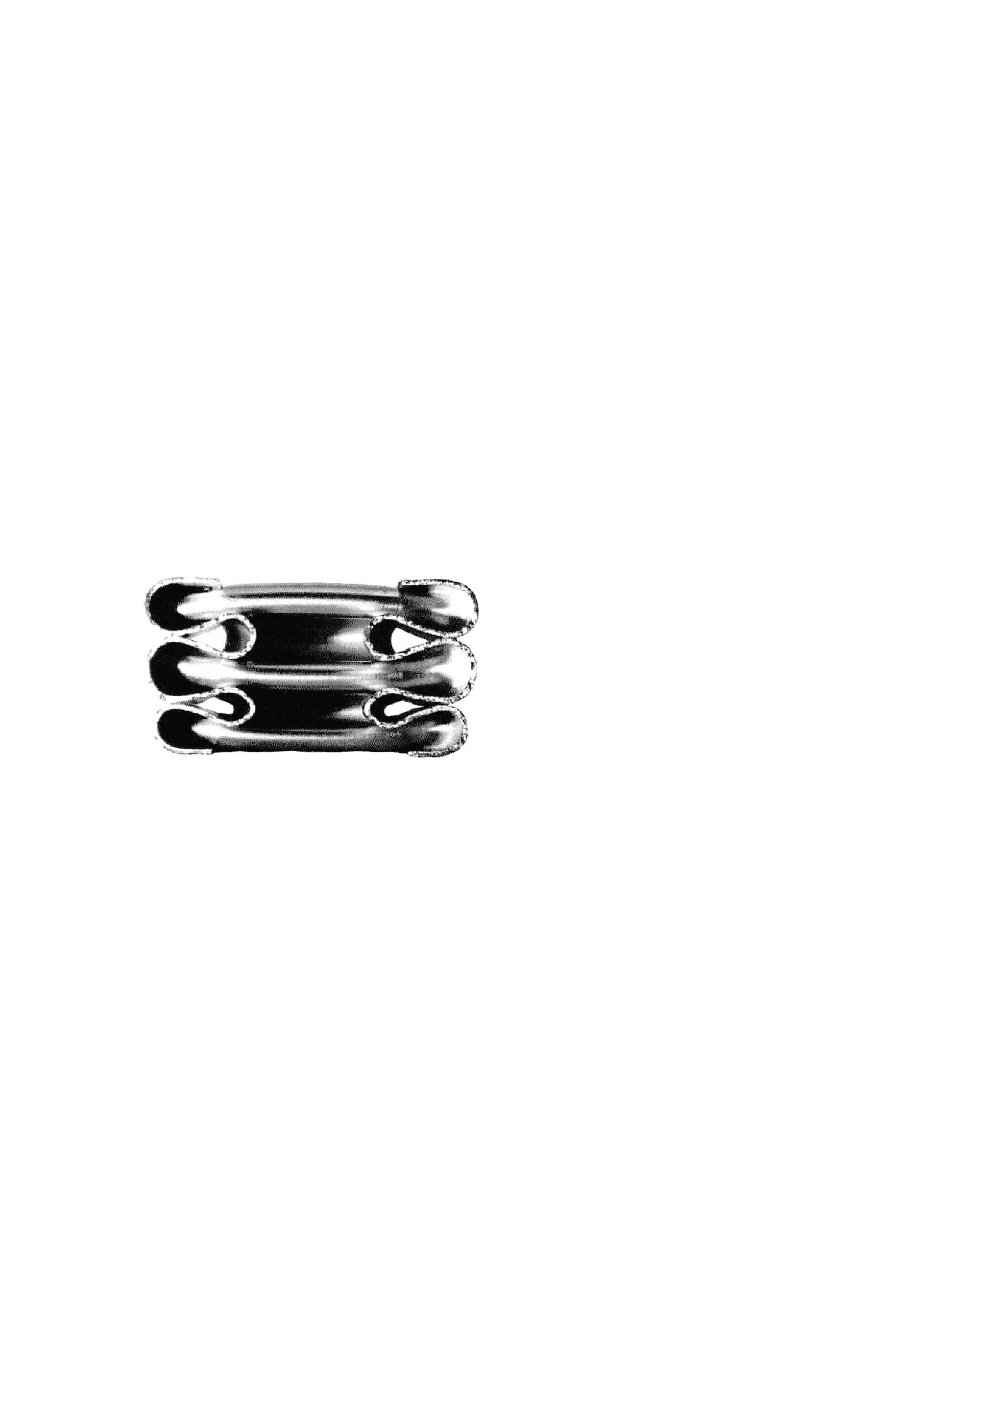
\includegraphics[width=0.7\linewidth]{./IMG_CUTRES/waves}
\caption[Waves formed on a crushed tube.]{Waves formed on a crushed tube. Taken from \citet{Langseth}.}
\label{fig:waves}
\end{figure}

It is in the wave formation process where another remarkable difference from the models tested by \citet{Scattina2011} takes place. In the present study, although waves develop sequentially as they were expected to, some simultaneity can be perceived on a certain length of the tube in some cases, like the one represented in \cref{fig:wave_form}. This is not considered binding of the validity of the model as, apart from happening on the impact head, wave formation may take also place in the opposite end of the tube or in some mid-point \citep{Abedrabbo2009, Costas2013} in this slender crash devices.

\begin{figure}
	\centering
%	\begin{minipage}[b]{.08\linewidth}
%		\centering
%		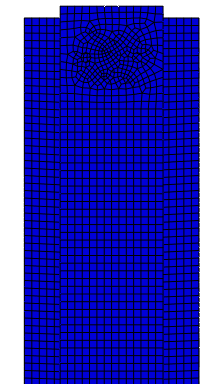
\includegraphics[width=\linewidth]{IMG_CUTRES/c0}
%	\end{minipage}
%	\quad
	\begin{minipage}[b]{.15\linewidth}
		\centering
		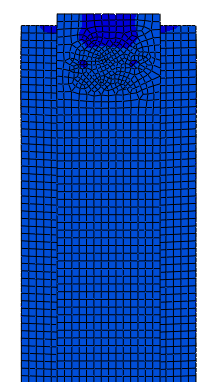
\includegraphics[width=\linewidth]{IMG_CUTRES/c1}
		$\SI{3}{\ms}$
	\end{minipage}
	\quad
	\begin{minipage}[b]{.15\linewidth}
		\centering
		\includegraphics[width=\linewidth]{IMG_CUTRES/c2}
		$\SI{6}{\ms}$
	\end{minipage}
	\quad
	\begin{minipage}[b]{.15\linewidth}
		\centering
		\includegraphics[width=\linewidth]{IMG_CUTRES/c3}
		$\SI{9}{\ms}$
	\end{minipage}
	\quad
	\begin{minipage}[b]{.15\linewidth}
		\centering
		\includegraphics[width=\linewidth]{IMG_CUTRES/c4}
		$\SI{12}{\ms}$
	\end{minipage}
	\quad
	\begin{minipage}[b]{.15\linewidth}
		\centering
		\includegraphics[width=\linewidth]{IMG_CUTRES/c5}
		$\SI{15}{\ms}$
	\end{minipage}
	\quad
	\begin{minipage}[b]{.15\linewidth}
		\centering
		\includegraphics[width=\linewidth]{IMG_CUTRES/c6}
		$\SI{18}{\ms}$
	\end{minipage}
	\quad
	\begin{minipage}[b]{.15\linewidth}
		\centering
		\includegraphics[width=\linewidth]{IMG_CUTRES/c7}
		$\SI{21}{\ms}$
	\end{minipage}
	\quad
	\begin{minipage}[b]{.15\linewidth}
		\centering
		\includegraphics[width=\linewidth]{IMG_CUTRES/c8}
		$\SI{24}{\ms}$
	\end{minipage}
	\quad
	\begin{minipage}[b]{.15\linewidth}
		\centering
		\includegraphics[width=\linewidth]{IMG_CUTRES/c9}
		$\SI{27}{\ms}$
	\end{minipage}
	\quad
	\begin{minipage}[b]{.15\linewidth}
		\centering
		\includegraphics[width=\linewidth]{IMG_CUTRES/c10}
		$\SI{30}{\ms}$
	\end{minipage}
\caption{Early stages of wave formation process on the impact head.}
\label{fig:wave_form}
\end{figure}

During the development of this study, several adherend thicknesses were tried as a manner of influence on the simultaneity/sequentiality of the wave formation. It was checked that thicker adherends were proner to develop sequentiality in this process, although other problems arise, as it is explained later.

\subsection{Critical situations}
\label{sec:critical_sits}
\citet{Peroni2009} found several situations in impact tests in which the expected collapse mechanism wasn't achieved. Instead, bonding rapidly failed, making almost only use of the plate's capabilities to absorb the impact through its elastic-plastic deformation like bending shells, usually without wave formation at all or only on a part of the tube.

When this situation takes place, \gls{Ea} may get drastically reduced, depending on several parameters. During the study development, it was found on several unprecise models ---i.e.: with minored adhesive properties--- that this critical situations can drop \gls{SEA} to a half or even a third of the expected values if compared with non-critical values given by \citet{Peroni2009} on their stable counterparts. In some cases, the general effect of this has less importance, as it will be shown. As previously explained, crash boxes fairly improve their response to this situation by fixing togheter the adherends plates with rivets \citep{Peroni2009}.

Critical situations also take place on \gls{FEM} models. \citet{Yang2012} found this happening on a double-hat hexagonal tube sujected to impact (\cref{fig:yangs_tube}) using a validated model with equivalent adhesive properties. \citet{Yamashita2013} also found this on impact tests and models of a top-hat tube, being the experimental and the modelled tests very similar in their results.

In this study, they were mainly found on double-hat square tubes, being the top-hat solution fairly more resistant to these problems.
% SELF EXAMPLE AND FIGURE

The importance of controlling this misfunctions also has to do with material efficiency, as the stable collapse mechanism reaches the greatest values of \gls{Ea}, with a reasonable control of \gls{Pk}.

In the present study, as previously stated, they were controlled by the addition of a stabilizing box and spot weld points in the flanges at the triggering cross section. Although they are not prevented completely, the general behaviour of the tube is fairly improved, as it gets closer to what is expected when comparing to \citet{Peroni2009} and \citet{Scattina2011}.

\begin{figure}
	\centering
	\includegraphics[width=0.9\linewidth]{IMG_CUTRES/yangs_tube}
	\caption[\Acrshort{FEM} analysis of a hexagonal crash box carried out by \citet{Yang2012}.]{\Acrshort{FEM} analysis of a hexagonal crash box carried out by \citet{Yang2012}. The begginning of tube's head opening can be seen on stage B, and it has totally peeled the adhesive layer by stage C.}
	\label{fig:yangs_tube}
\end{figure}

Using the scripting capabilities of the developed model, an hexagonal crash tube was tested. The collapse process of this section in the developed model is fairly prone to trigger missfunction, and it highly resembled the problems that \citet{Yang2012} found in the simulation.

% Insert figure & comment

This section aims to expose some of the most common critical situations found during the study development, usually by changing the boundary conditions affecting the tube. The reasons involved in this malfunctioning are related and always present combined, and were subducted by the addition of rivets and a stabilizing box to the model (\cref{sec:impact}).

\subsubsection{Triggering missfunctions}  % Head aperture
\label{sec:trig_missf}

Without the eventually included rivets, depending on the adherend thickness ---specifically for low values of this parameter---, triggering could not work properly: an excesive bending takes place at that point in the bonding flanges, together with little bending on points close to that part of the tube. In addition, this deformations happen to lead to opening the section.

This aperture may be caused either by a tendency to form waves with stiffer ---due to their undeformed state--- sections next to it which restrain this collapse mechanism on that point, or either by the presence of symmetrical wave patterns instead of parallel wave patterns leading to a wave in each adherend trying to open the section next to the trigger. Both situations may coexist, but either of them provokes the adhesive failure by pure mode I loading.

Failure may happen on the triggered cross section (see \cref{fig:trig_misf_A}, in this study, this was solved by using spot weld points in that cross section) or on the mid-tube (see \cref{fig:trig_misf_mid}). In this last case, general bending may also take place afterwards.

\begin{figure}
	\centering
	\begin{minipage}[b]{.65\linewidth}
		\includegraphics[width=\linewidth]{IMG_CUTRES/trig_misf_A1}
	\end{minipage}
	\quad
	\begin{minipage}[b]{.65\linewidth}
		\includegraphics[width=\linewidth]{IMG_CUTRES/trig_misf_A2}
	\end{minipage}
	\quad
	\begin{minipage}[b]{.65\linewidth}
		\includegraphics[width=\linewidth]{IMG_CUTRES/trig_misf_A3}
	\end{minipage}
	\caption{Trigger misfunction development on a top-hat section crash tube at $\SI{1.5}{\ms}$, $\SI{4.5}{\ms}$ and $\SI{15}{\ms}$.}
	\label{fig:trig_misf_A}
\end{figure}

\begin{figure}
	\centering
	\includegraphics[width=0.7\linewidth]{IMG_CUTRES/trig_misf_mid}
	\caption[View cut detail of a double hat section crash tube with triggering misfunction initiation on a middle point.]{View cut detail of a double hat section crash tube with triggering misfunction initiation on a middle point. Focus on the symmetrical bending wave pattern. Adhesive in blue.}
	\label{fig:trig_misf_mid}
\end{figure}

%\begin{figure}
%	\centering
%	\includegraphics[width=.7\linewidth]{IMG_CUTRES/tmfB_detail}
%	\caption{Detail of a double hat section tube head in which triggering missfunction is starting to develop.}
%	\label{fig:tmfB_detail}
%\end{figure}

\begin{figure}
	\centering
	\begin{minipage}[b]{.22\linewidth}
		\centering
		\includegraphics[width=\linewidth]{IMG_CUTRES/tmf1}
		$\SI{0.6}{\ms}$
	\end{minipage}
	\quad
	\begin{minipage}[b]{.22\linewidth}
		\centering
		\includegraphics[width=\linewidth]{IMG_CUTRES/tmf2}
		$\SI{1.05}{\ms}$
	\end{minipage}
	\quad
	\begin{minipage}[b]{.22\linewidth}
		\centering
		\includegraphics[width=\linewidth]{IMG_CUTRES/tmf3}
		$\SI{1.5}{\ms}$
	\end{minipage}
	\quad
	\begin{minipage}[b]{.22\linewidth}
		\centering
		\includegraphics[width=\linewidth]{IMG_CUTRES/tmf4}
		$\SI{1.95}{\ms}$
	\end{minipage}
	\caption[Triggering missfunction development process on a double hat section crash tube.]{Triggering missfunction development process on a double hat section crash tube. Adhesive in blue.}
	\label{fig:tmf}
\end{figure}

By facing \cref{fig:tmf}, it is supposed that this situation has its origin on an adherend thickness-triggering relation that also depends on the cross section of the tube, as the plates initial bend is allowed by the reduced adherend thickness and this is the origin of the peeling failure due to the plates bending directionality, which tends to open the union from the inside. After this situation has started, the more the head is deformed, the more it is developed. There are several other arguments supporting this theory:
\begin{itemize}
	\item The lack of triggering also leads to this situation.

	\item Hexagonal cross sections \citep{Yang2012} are particulary prone to develop this critical situation.

	\item Thicker adherends seem to be about of avoiding this misfunction before starting other critical collapse mechanisms.

	\item It is the main critical situation that can be found on top-hat cross section crash tubes.
\end{itemize}

\Cref{fig:tmf_fd} shows the corresponding force-displacement curve of the tube of \cref{fig:tmf}. In this critical situation, adherends start to bend over a certain point of the tube provoking the peeling along the tube in the process. The second peak present in \cref{fig:tmf_fd} may be motivated by the impact plate reaching this bending point and thus starting an in-plane compression of the adherends like the experienced in the beginning.

\begin{figure}
	\centering
	\includegraphics[width=0.7\linewidth]{IMG_CUTRES/tmf_fd}
	\caption{Force-displacement curve for a crash tube with triggering missfunction.}
	\label{fig:tmf_fd}
\end{figure}

This misfunction is also particularly independent of the tube length, as the analysis with different values of this parameter showed. This situation is also particularly easy to be developed on hexagonal crash boxes, as \cref{fig:hex_tmf} shows.

\begin{figure}
	\centering
	\begin{minipage}[b]{.3\linewidth}
		\centering
		\includegraphics[width=\linewidth]{IMG_CUTRES/hex1}
		$\SI{0.6}{\ms}$
	\end{minipage}
	\quad
	\begin{minipage}[b]{.3\linewidth}
		\centering
		\includegraphics[width=\linewidth]{IMG_CUTRES/hex2}
		$\SI{1.2}{\ms}$
	\end{minipage}
	\quad
	\begin{minipage}[b]{.3\linewidth}
		\centering
		\includegraphics[width=\linewidth]{IMG_CUTRES/hex3}
		$\SI{1.8}{\ms}$
	\end{minipage}
	\caption[Triggering missfunction development process on a hexagonal cross section crash tube.]{Triggering missfunction development process on a hexagonal cross section crash tube. Adhesive in blue.}
	\label{fig:hex_tmf}
\end{figure}

\subsubsection{General bending}

It was found that in many cases, during the wave formation process, a minor difference between plates deformation, eventually resulted in the box bending by some mid-point, diverting the tube's directrix instead of crushing the device in a straight direction (see \cref{fig:general_bending}).

\begin{figure}
	\centering
	\begin{minipage}[b]{.7\linewidth}
		\includegraphics[width=\linewidth]{IMG_CUTRES/general_bending_73}
	\end{minipage}
	\quad
	\begin{minipage}[b]{.3\linewidth}
		\includegraphics[width=\linewidth]{IMG_CUTRES/general_bending_48}
	\end{minipage}
	\quad
	\begin{minipage}[b]{.3\linewidth}
		\includegraphics[width=\linewidth]{IMG_CUTRES/general_bending_72}
	\end{minipage}
	\quad
	\begin{minipage}[b]{.3\linewidth}
		\includegraphics[width=\linewidth]{IMG_CUTRES/general_bending_55}
	\end{minipage}
\caption[Final deformation status of a double hat section crash tube model without stabilizing box in a general bending critical situation.]{Final deformation status of a double hat section crash tube model without stabilizing box in a general bending critical situation. Crushing from the left.}
\label{fig:general_bending}
\end{figure}

Analyzing the origin of this situation, several possible reasons were considered:
\begin{itemize}
	\item A longer wave on one side, followed by a less pronounced one. Membrane effect on the former one makes it a stiffer point. The last one is a weak section, as the consecutive adherend planes are folding together. As this situation only takes place on one of the adherends, the faux-symmetry ceases to exist, thus bending the tube by some mid-point.

	\item Following a behaviour similar to that one found in triggering missfunction, aperture of the section happens in some mid-point. Usually an excesively opened wave by the union plane, sided by two under-formated waves that cannot compensate the aperture, triggers this failure.
\end{itemize}

This situation usually takes place with minor adhesive failure on its initial phases, and rapidly failing in a peel-shear combination when the bend is completely formed on almost the whole surface.

Ideal bonding ---using tie constraints instead of a material union--- presented this collapse mechanism, only differing in the last phases, depicted in \cref{fig:general_bending}, in which the adhesive fails.

This suggests that the adhesive meets its objective on retainning the two flanges together, at least until the critical failure has completely developed itself, and thus suggesting an adherend or trigger origin of this problem.

It also suggests that the adhesive influence on the general response is of little importance on the last phases, meaning that once the critical situation is initiated, the response barely depends on the bond.

On the other hand, top-hat section crash tubes were found to be fairly more resistant to developing this kind of malfunction, as no cases were found.

\subsubsection{General peeling due to plates buckling}

Excessively thick adherend plates prevent wave formation, resulting in other collapse mechanisms development, such as a buckling-like deformation, as a slender beam subjected to high compression. In this situation, each plate bends to a side, peeling the union in the process. In this situation, the stiffness difference between adherend and adhesive results in a behaviour that could be described as if the former impossed deformations to the later.

Although it could not be measured, it is supposed that a big share part of the \gls{Ea} value comes from elastic-plastic deformation of the adherend plates. The adhesive failure is purely mode I, and thus only the corresponding fracture energy is absorbed, which is recalled that was about one fifth of the other modes value. In spite of that, \gls{SEA} values with $\SI{2}{\mm}$ plate thickness were close to the ones found with $\SI{1}{\mm}$ carried out by \citet{Peroni2009} with a stable collapse mechanism.

\begin{figure}
	\centering
	\begin{minipage}[b]{.48\linewidth}
	\centering
	\begin{minipage}[b]{\linewidth}
		\centering
		\includegraphics[width=\linewidth]{IMG_CUTRES/gppb67}
		$\SI{2.0}{\ms}$
	\end{minipage}
	\quad
	\begin{minipage}[b]{\linewidth}
		\centering
		\includegraphics[width=\linewidth]{IMG_CUTRES/gppb84}
		$\SI{2.5}{\ms}$
	\end{minipage}
	\quad
	\begin{minipage}[b]{\linewidth}
		\centering
		\includegraphics[width=\linewidth]{IMG_CUTRES/gppb100}
		$\SI{3.0}{\ms}$
	\end{minipage}
	\end{minipage}
	\quad
	\begin{minipage}[b]{.48\linewidth}
		\centering
		\includegraphics[width=\linewidth]{IMG_CUTRES/gppb300}
		$\SI{9.0}{\ms}$
	\end{minipage}

	\caption{General peeling due to plates buckling collapse process.}
	\label{fig:gppb}
\end{figure}

This fact may be used as an argument to make the adherends thicker, but the \acrlong{Pk} was also strongly increased to over $\SI{100}{\kN}$ in this case as it can be seen on \cref{fig:gppb_fd}, which is undesirable. In that same figure, it can be seen how the pure mode I failure of the whole adhesive allows little energy aborption. \Gls{SEA} is $\SI{4.28}{\kJ/\kg}$, lower than other solutions due to this inefficiency.

\begin{figure}
	\centering
	\includegraphics[width=0.7\linewidth]{IMG_CUTRES/gppb_fd}
	\caption{\Acrlong{F-D} for a $\SI{2}{\mm}$ adherend thick in which general peeling due to plates buckling is developed.}
	\label{fig:gppb_fd}
\end{figure}

Unlike the commented triggering missfunction, general peeling finds its origin on a buckling-like behaviour of the plates which produces the peeling, while the malfunction of the trigger leads to local failure of the bonding, leading to the rotation of a part of the plate arround a wave formed in a rearer point of the tube. In addition, triggering missfunction is easier to develop with lower thickness values, while general peeling is produced with higher values of this parameter.

\section{Interpretation}  % Include different geoms comparation if possible
\label{sec:interpretation}

In general terms, top-hat section tubes betterly resemble the reference crash boxes, specially due to their higher resistance to develop undesired collapse mechanisms.

\subsection{Stable collapse mechanism}

\Cref{fig:stable} depicts the collapse sequence of a top-hat crash tube, showing a stable crushing pattern. Analyzing the modellization, it can be concluded that this collapse was achieved thanks the stabilizing box, as it retains the plates at certain points. \Cref{fig:stabil_box} depicts the final state of the crushing process, showing how the stabilization box retained the crash tube.

\begin{figure}
	\centering
	\begin{minipage}[b]{.06\linewidth}
		\centering
		\includegraphics[width=\linewidth]{IMG_CUTRES/a0}
	\end{minipage}
	\quad
	\begin{minipage}[b]{.06\linewidth}
		\centering
		\includegraphics[width=\linewidth]{IMG_CUTRES/a1}
	\end{minipage}
	\quad
	\begin{minipage}[b]{.06\linewidth}
		\centering
		\includegraphics[width=\linewidth]{IMG_CUTRES/a2}
	\end{minipage}
	\quad
	\begin{minipage}[b]{.06\linewidth}
		\centering
		\includegraphics[width=\linewidth]{IMG_CUTRES/a3}
	\end{minipage}
	\quad
	\begin{minipage}[b]{.06\linewidth}
		\centering
		\includegraphics[width=\linewidth]{IMG_CUTRES/a4}
	\end{minipage}
	\quad
	\begin{minipage}[b]{.06\linewidth}
		\centering
		\includegraphics[width=\linewidth]{IMG_CUTRES/a5}
	\end{minipage}
	\quad
	\begin{minipage}[b]{.06\linewidth}
		\centering
		\includegraphics[width=\linewidth]{IMG_CUTRES/a6}
	\end{minipage}
	\quad
	\begin{minipage}[b]{.06\linewidth}
		\centering
		\includegraphics[width=\linewidth]{IMG_CUTRES/a7}
	\end{minipage}
	\quad
	\begin{minipage}[b]{.06\linewidth}
		\centering
		\includegraphics[width=\linewidth]{IMG_CUTRES/a8}
	\end{minipage}
	\quad
	\begin{minipage}[b]{.06\linewidth}
		\centering
		\includegraphics[width=\linewidth]{IMG_CUTRES/a9}
	\end{minipage}
	\quad
	\begin{minipage}[b]{.06\linewidth}
		\centering
		\includegraphics[width=\linewidth]{IMG_CUTRES/a10}
	\end{minipage}

	\caption[Stable collapse mechanism achieved in the top-hat tube with stabilizing box.]{Stable collapse mechanism achieved in the top-hat tube with stabilizing box. Semi-transparent projection with adhesive in red. Total time: $\SI{15}{\ms}$; uniform spacing.}
	\label{fig:stable}
\end{figure}

\begin{figure}
	\centering
	\includegraphics[width=.7\linewidth]{IMG_CUTRES/parallel_stable}
	\caption{Final state on parallel projection with the stabilizing box represented.}
	\label{fig:stabil_box}
\end{figure}

Reaction force is analyzed in this case in order to check the importance share of the stabilizing box on achieving this result. Its \acrlong{F-D} is displayed in \cref{fig:stabil_F}, with an equivalent \gls{SEA} of $\SI{0.30}{\kJ/\kg}$ and peaks of up to $\SI{4.4}{\kN}$. This force has one only component, parallel to the Y axis, which is reminded to be normal to the crushing direction and to the bonding flanges.

\begin{figure}
	\centering
	\includegraphics[width=.7\linewidth]{IMG_CUTRES/RF2_stable}
	\caption{Reaction force on the stabilizing box.}
	\label{fig:stabil_F}
\end{figure}

According to the results displayed on \cref{fig:stable,fig:stabil_box,fig:stabil_F}, it can be concluded that the stabilizing box helps on providing an stable collapse mechanism to the crash tube through the inclusion of a certain force with a minimum \gls{SEA} input to the system.

\subsection{Factors on absorption of energy}
\label{sec:Ea_factors}

Facing the \gls{F-D} and different collapse states at several time intervals, an analysis on the relative importance of each factor on \gls{Ea} is carried out.

The in-plane compression of the rear un-collapsed part of the tube, together with plastic deformation of the frontal end, are the main actors on the base reaction force ---a minimum maintained level that keeps its value almost constant and leaving the variable part to other factors.

Bending waves \textit{per se} do not have great influence on the peaks and valleys series of the \gls{F-D}, but the adhesive failure pattern does, and it is determined by the former. This means that it is not the adherend plastic deformation the main factor of this variable part, although it has certain variability. \Cref{fig:ads_collapse_progresion} is the case in which this phenomenom can be most easily perceived, as in certain moment, adhesive rapidly fails with very little adherend deformation, and highly increasing the reaction force.

In that same figure, the peak between $\SI{8.25}{\ms}$ and $\SI{10.2}{\ms}$ corresponds to some adhesive final failure (depicted by element removal in the first and second states). The same applies more drastically between the third and fourth states, depicting $\SI{13.2}{\ms}$ and $\SI{15.0}{\ms}$ respectively.

This analysis can be carried out for any other case, with the same conclusions, although this one is the most graphical and the easiest one to be percerived.

\begin{figure}
	\centering
	\begin{minipage}[b]{.35\linewidth}
		\centering
		\begin{minipage}[b]{\linewidth}
		\includegraphics[width=\linewidth]{IMG_CUTRES/AR_RSB_8-25}
		\end{minipage}
		\quad
		\begin{minipage}[b]{\linewidth}
		\includegraphics[width=\linewidth]{IMG_CUTRES/AR_RSb_10-2}
		\end{minipage}
		\quad
		\begin{minipage}[b]{\linewidth}
		\includegraphics[width=\linewidth]{IMG_CUTRES/AR_RSb_13-2}
		\end{minipage}
		\quad
		\begin{minipage}[b]{\linewidth}
		\includegraphics[width=\linewidth]{IMG_CUTRES/AR_RSb_15}
		\end{minipage}
	\end{minipage}
	\quad
	\begin{minipage}[b]{.6\linewidth}
		\includegraphics[width=\linewidth]{IMG_CUTRES/AR_RSb}
	\end{minipage}
\caption[Adhesive collapse influence on \acrlong{F-D}.]{Adhesive collapse influence on \acrlong{F-D}. Collapse states with semi-transparent adherends and adhesive in red at $\SI{8.25}{\ms}$, $\SI{10.2}{\ms}$, $\SI{13.2}{\ms}$, and $\SI{15.0}{\ms}$; and corresponding \gls{F-D}. In this case, collapse is started by a mid-point.}
\label{fig:ads_collapse_progresion}
\end{figure}

The possible critical situations that can be developed as a collapse mechanism have varying importance on the final results, strongly depending on the cross section. As commented on \cref{sec:critical_sits}, top-hat section presents minor \gls{SEA} losses and is more resistant to developing this missfunctions, unlike double hat section.

As of this, it can be concluded that there are three main factors influencing on the value of \gls{Ea}, being these, in order of importance:
\begin{itemize}
	\item Adherend properties: more specifically its geometry and material.
	\item Adhesive characteristics: specially those involved in its failure, like the fracture energy.
	\item Missfunctional behaviour: although in some cases may be negligible, in others it can be determining.
\end{itemize}

Finally, \cref{tab:sea} summarizes the different obtained \gls{SEA} values. From there, it can be seen how the top-hat section is not affected in the same magnitude in the final \gls{SEA} value as the double hat section, although the collapse mechanism may change by transfering the wave formation process to other part of the tube and certain other corresponding implications. The obtained values are close to those experimentally obtained by \citet{Peroni2009}, giving certain credit on the goodness of the results of the present study.

On the other hand, the double hat section \gls{SEA} obtained values drastically change when modifying the contact interaction properties, dropping to between $82\%$ and $63\%$ of values with other interaction definition, and about a half or even a third of the experimental values obtained by \citet{Peroni2009}. The rough case with stabilization box seems to get the closest to resembling cited experiments, although its collapse mechanism is not the same, as the modelled one generates waves in the mid-tube, as can be seen on \cref{fig:best_B_tube}

\begin{figure}
	\centering
	\includegraphics[width=0.7\linewidth]{IMG_CUTRES/best_B_tube}
	\caption[Collapse of the double hat section tube with stabilization box and rough contact property.]{Collapse of the double hat section tube with stabilization box and rough contact property. Adhesive in blue. \Gls{SEA}: $\SI{7.34}{\kJ/\kg}$.}
	\label{fig:best_B_tube}
\end{figure}


\begin{table}[htpb]
	\centering
	\begin{tabular}{llcc}
		\toprule
		\multirow{2}{*}{Contact} & \multirow{2}{*}{Situation} & \multicolumn{2}{c}{Cross section} \\ \cmidrule{3-4}
		\multicolumn{2}{l}{}                                    & Top-hat         & Double hat     \\ \midrule
		\multirow{4}{*}{Rough}                  & -             & $5.43$          & $5.20$         \\
		& R             & $5.36$          & $6.08$          \\
		& Sb            & $5.70$          & $7.34$          \\
		& RSb           & $5.61$          & $6.69$          \\ \midrule
		\multirow{4}{*}{Frictionless}           & -             & $4.21$          & $3.32$         \\
		& R             & $5.50$          & $3.86$         \\
		& Sb            & $5.55$          & $5.88$          \\
		& RSb           & $5.40$          & $5.51$          \\ \bottomrule
	\end{tabular}
	\caption[\Acrlong{SEA} summary.]{\Acrlong{SEA} summary. ``R'' stands for riveted tube; ``Sb'', for tube with stabilizing box; ``RSb'', for both simultaneously.}
	\label{tab:sea}
\end{table}

\subsection{On load standard deviation}

Facing the factors that were concluded on \cref{sec:Ea_factors}, the \gls{SD} value of the \gls{F-D} can be interpreted also as a measure of the progressiveness or the suddenness of the failure of the crash box, specially and more specifically of the adhesive.

\begin{table}[htpb]
	\centering
	\begin{tabular}{llcc}
		\toprule
		\multirow{2}{*}{Contact} & \multirow{2}{*}{Situation} & \multicolumn{2}{c}{Cross section} \\ \cmidrule{3-4}
		\multicolumn{2}{l}{}                                    & Top-hat         & Double hat      \\ \midrule
		\multirow{4}{*}{Rough}                  & -             & $6.79$          & $10.47$         \\
		& R             & $6.60$          & $8.84$          \\
		& Sb            & $8.04$          & $6.80$          \\
		& RSb           & $7.25$          & $7.73$          \\ \midrule
		\multirow{4}{*}{Frictionless}           & -             & $5.76$          & $11.91$         \\
		& R             & $5.53$          & $10.72$         \\
		& Sb            & $5.29$          & $8.65$          \\
		& RSb           & $4.97$          & $8.82$          \\ \bottomrule
	\end{tabular}
	\caption[\Acrlong{SD} summary.]{\Acrlong{SD} summary. ``R'' stands for riveted tube; ``Sb'', for tube with stabilizing box; ``RSb'', for both simultaneously.}
	\label{tab:standard_dev}
\end{table}

In general terms, top-hat section shows a better performance in terms of \gls{SD}, as it can be seen on \cref{tab:standard_dev}, likely thanks to its better resistance to developing critical situations. Both rough cases with stabilizing box on rough contact conditions seem to be the exception to the tendency, as the top-hat tube shows a larger \gls{SD} than the double hat one. Their \gls{F-D} is depicted in \cref{fig:R_Sb}. A similar phenomenom happens on those cases that add rivets to these ones, although not in an enough magnitude to make the double hat section value bigger than the top-hat section one.

\begin{figure}
	\centering
	\includegraphics[width=0.7\linewidth]{IMG_CUTRES/R_Sb}
	\caption{\Acrlong{F-D} of models with rough contact and stabilizing box.}
	\label{fig:R_Sb}
\end{figure}

Although none of these cases depicts a critical situation, they behave differently to other similar tests. Analyzing the collapse mechanism in the top-hat section, the rapid mode II failure at certain stages creates local peaks also explained in \cref{sec:final_tendency} that are related to the variability of the \gls{F-D}.

Concurring with this situation, on the other hand, the double hat section shows in these cases some of the most stable collapses among the obtained results, allowing thus a more balanced result against its counterpart. In spite of being fairly stable, its \gls{SD} is still particularly high if compared to many top-hat section results. Analyzing the \gls{F-D}, the peaks and valleys series is included in a general downwards tendency, unlike other series which oscilate among a fairly constant level. This implies that \gls{SD} is not the perfect tool for measuring the stability of the collapse mechanism, although it is good enough to give an idea.

Double hat section on frictionless contact conditions, whose \gls{F-D} are represented in \cref{fig:F-D_frictionless}, present the greatest values of \gls{SD} among the modelled tubes. In spite of the similarities between these curves, the showed collapse mechanism is different between those with and without stabilizing box, although the causes are fairly the same: a great valley after the \acrlong{Pk} followed by a second local peak arround $\num{8}\sim\SI{10}{\ms}$.

The cases without stabilizing box find the genesis of this late peak in the developed critical situation, which corresponds to a general bending case. As \cref{fig:gen_bend_weakening} shows, the peak implies the final dispossure of \gls{Ea} by the frontal part of the tube, as it completely bends over itself. Beyond this point, this frontal part does not intervene any more, and the collapse starts again in some way from this moment only using the capabilities of the rest of the tube.

\begin{figure}
	\centering
	\begin{minipage}[b]{.3\linewidth}
		\centering
		\includegraphics[width=\linewidth]{IMG_CUTRES/b1}
		$\SI{7.5}{\ms}$
	\end{minipage}
	\quad
	\begin{minipage}[b]{.3\linewidth}
		\centering
		\includegraphics[width=\linewidth]{IMG_CUTRES/b2}
		$\SI{8.25}{\ms}$
	\end{minipage}
	\quad
	\begin{minipage}[b]{.3\linewidth}
		\centering
		\includegraphics[width=\linewidth]{IMG_CUTRES/b3}
		$\SI{9.0}{\ms}$
	\end{minipage}
	\caption[Final collapse dispossure of the frontal part of the tube in a general bending case.]{Final collapse dispossure of the frontal part of the tube in a general bending case. Adhesive in blue.}
	\label{fig:gen_bend_weakening}
\end{figure}

In those cases with stabilizing box, this process aims to develop, but it is stopped by the mentioned device, which does not prevent the second peak. Big bending waves are developed within the stabilizing box on its place. After the great valley between $\SI{2}{\ms}$ and $\SI{7}{\ms}$, approximatedly, force values scale up back again, finding a second peak with similar origin and characteristics as the one mentioned for the previous case. From that point, more energy is absorbed mainly due to adhesive failure. In the final stages, the currently forming wave implodes the cross section. In general terms, this collapse mechanism is fairly chaotic ---as local collapse patterns change from one point to another instead of developing the same in the whole tube---, in spite of being stabilized.

\subsection{Final raising tendency}
\label{sec:final_tendency}
% Explain tendency on the final stages to great values

Several models with stabilizing box and rough contact were found to scale up the transmitted load in the last stages of the impact, thus deviating from the reference values, and reaching values close to the \acrlong{Pk} that takes places in the first moments of the impact. \Gls{F-D} of this models are depicted in \cref{fig:AR_Sb}.

\begin{figure}
	\centering
	\includegraphics[width=0.7\linewidth]{IMG_CUTRES/AR_Sb}
	\caption{Top-hat section models with rough contact developing high values of transmitted load in the last stages of the impact.}
	\label{fig:AR_Sb}
\end{figure}

Analyzing the collapse path, this tubes show wave formation in the mid-rear part of the tube. The wave size has relation with the big peak of the middle of the analysis. The frontal part of the box seems to enter an in-plane compression of the adherends in the last phases of the impact, with high shear effort between adherends.

This leads to a rapid energy release due to adhesive mode II failure in the last moments of the analysis, likely creating the last peak of the analysis.

Although the final \gls{Ea} is relatively similar to other cases, this last peak on loading is considered totally underisable, as it reaches values of more than $80\%$ of \gls{Pk} which would increase injury suffered by vehicle passengers.

\subsection{Model deviations}
The present section aims to expose some of the differences found between the developed models and the results of reference given mainly by \citet{Scattina2011} and \citet{Peroni2009}.

Obtained curves present a first peak of $\num{45}\sim\SI{50}{\kN}$ in the beginning of the impact, and then a series of peaks, less pronounced and lower in value, alternating with valleys during the wave formation, with a mean value of $\num{10}\sim\SI{20}{\kN}$. Reference values were found to be alike, being the main exception on the double-hat section, which has lower peak and mean force value.

The main exception to these similitudes can be found on the first peak, specially with rough interaction property, which progressively reduces its value after happening, instead of rapidly dropping its magnitude to the peaks and valleys series' mean. It is believed that this situation may be related to the crushing speed. On a quasi-static experiments and models, test velocity allows stresses to reaccommodate; meanwhile, on impact tests, this redistribution can be appreciatted thanks to the scale of time.

\subsection{Critical situations results}

\Cref{tab:critical_sits} summarises the \gls{SEA} values obtained in the present study for the different critical situations that were experienced. As shown, top-hat section crash boxes decay less when happenning, being thus much more reliable solution for this use.

\begin{table}
	\centering
	\begin{tabular}{lcc}
		\toprule
		Critical situation 						& Top-hat 		& Double hat 	\\
		\midrule
		None 									& $\num{5.55}$	& $\num{7.34}$ 	\\
		Triggering misfunction 					& $\num{4.21}$	& $\num{5.13}$ 	\\
		General bending 						& Unfound		& $\num{4.79}$ 	\\
		General peeling due to plates buckling 	& Unfound		& $\num{4.28}$ 	\\
		\bottomrule
	\end{tabular}
	\caption[Summary of \acrshort{SEA} values on different critical situations.]{Summary of \acrshort{SEA} [$\si{\kJ/\kg}$] values on different critical situations. Mean values given in case of being found several times. \citet{Peroni2009} obtained $\SI{4.8}{\kJ/\kg}$ and $\SI{10.3}{\kJ/\kg}$ respectively for top-hat and double hat sections.}
	\label{tab:critical_sits}
\end{table}

It is also very remarkable the significantly high values of \gls{SD} in this situations, motivated by the strong variabilities in their corresponding force-displacement curves (see \cref{fig:tmf_fd,fig:gppb_fd}).

In case of triggering missfunction, it reaches $\SI{11.66}{\kJ/\kg}$, a value alike the most unfavorable found in this study. The general peeling due to plates buckling case is $\SI{32.99}{\kJ/\kg}$. It should be remarked that, because of the definition of this parameter, this value is not as high as it may look like, as the mean values of these both force-displacement curves is $\SI{14.78}{\kJ/\kg}$ and $\SI{28.76}{\kJ/\kg}$, respectively.

\chapter{Conclusions}

The following conclusions were deduced from the results of this study:
\begin{itemize}
	\item Impact speed conditions are key parameters on determining the resulting adhesive failure manner and general collapse mechanism. Appropiate triggering systems are necessary in order to develop collapse mechanisms capable of absorbing the most of energy.

	\item Quasi-static experiments are the most widely spread tests among literature, altough resulting collapses are very different on impact conditions.

	\item In spite of having improved adhesive resistance in the last years, peeling strength is still a widely developed failure mode in the modelled crash tubes.

	\item Peeling usually starts from the inside of the tube to the outtermost part of the flanges, giving this an idea of where reinforcements should be applied.

	\item Damage is more continuous and progressive than other solutions because of bonding whole surfaces instead of a certain number of points like in a spot weld union, which present a more discrete behaviour.

	\item However, zip failure effect is still present, meaning that failure of a zone of the union makes neighbour zones more prone to get damage, or even fail, as load is increased on them.

	\item Unexpected collapse mechanisms suppose an important type of response of the crash box. When happening, \gls{SEA} may be reduced to a half or even a third of expected, and standard deviation scales up.

	\item The stiffness difference between adhesive and adherends implies that, in some way, adherends impose displacements to the adhesive once failure has started and near the failure front.

	\item The asymmetry of the top-hat section is an advantage for the collapse mechanism, as it gives the tube one plate strong enough to avoid certain critical behaviours and supresses the inconvenient interference between plates by being the other one the weak part of the tube.

	\item In relation with the previous point, the ``strong'' plate is resistant enough that, in case of critical situation, \gls{SEA} is still reduced, but in a much lesser magnitude.
\end{itemize}

\section{Future research lines}

Beyond this point, the optimization of the crash box using the developed code presents itself as one of the main lines continuing the present work. Other future research lines could include:

\begin{itemize}
	\item Change the crash box geometry trying to achieve regular collapses, avoiding unexpected collapse mechanisms, so energy absorption is maximized.

	\item Comparison with other joining solutions, such as laser weld.

	\item Inclusion of other adhesives and adherends in the study, enlarging the material database of the code.

	\item Improvements to the code ---such as including other triggering systems--- in order to deepen on crash box design and optimization.

	\item Applying of  adhesive bonding to other devices, even in other fields different from the automotive.
\end{itemize}

\printbibliography

\appendix

\chapter{Manufacturer's catalog information}
\label{apx:manuf}

\includepdf{IMG_CUTRES/catalog_1.pdf}
\includepdf{IMG_CUTRES/catalog_2.pdf}
\includepdf{IMG_CUTRES/catalog_3.pdf}

\chapter{Script code}
\label{apx:script}

\inputminted[breaklines=true, fontsize=\footnotesize]{python}{codes/paramodel.py}


\end{document}
